\documentclass[UTF8, fontset=macnew, a4paper, 12pt]{ctexart}

\usepackage{geometry}
\geometry{top=2.5cm, bottom=2.5cm, left=2.5cm, right=2.5cm}
\usepackage{amsmath, amssymb}
\usepackage{booktabs}
\usepackage{multirow}
\usepackage{tabularx}
\usepackage{graphicx}
\usepackage{caption}
\usepackage{xcolor}
\usepackage{float}
\usepackage{enumitem}
\usepackage{fancyhdr}
\usepackage{setspace}
\usepackage{pifont}
\usepackage{natbib}
% 拉丁作者名之後採半形括號（中文作者名在書目的中文部分仍用全形）；
% 第五個引數留空表示作者與年份之間不加逗號。
\bibpunct{(}{)}{; }{a}{}{,}
\usepackage[hidelinks]{hyperref}

\graphicspath{{../output/figures/}}
\captionsetup{font=small, labelfont=bf, labelsep=quad}
\setlist{itemsep=2pt, parsep=0pt, topsep=4pt}
\onehalfspacing

% ctexart 預設的圖表標號前綴為簡體「图」，改回正體。
\renewcommand{\figurename}{圖}
\renewcommand{\tablename}{表}

\ctexset{
  section/format = \raggedright\zihao{4}\bfseries,
  section/name   = {},
  section/number = \bignum{\value{section}},
  section/aftername = 、,
  subsection/format = \raggedright\zihao{5}\bfseries,
  subsection/number = \chinese{subsection},
  subsection/aftername = 、,
  subsubsection/format = \raggedright\normalsize\bfseries,
}
\newcommand{\bignum}[1]{\ifcase#1\or 壹\or 貳\or 參\or 肆\or 伍\or
  陸\or 柒\or 捌\or 玖\or 拾\fi}
\renewcommand{\thesection}{\bignum{\value{section}}}
% 交叉引用子節時補上節次，否則 \ref 只印出「三」而無從判斷屬於哪一節。
\renewcommand{\thesubsection}{\chinese{subsection}}
\makeatletter
\renewcommand{\p@subsection}{\thesection 節之}
\makeatother
\setcounter{secnumdepth}{2}

\pagestyle{fancy}
\fancyhf{}
\fancyhead[L]{}
\fancyhead[R]{\small 進度報告（1005 V2）}
\fancyfoot[C]{\small \thepage}
\renewcommand{\headrulewidth}{0.4pt}

% U+2460~2463 不在 xeCJK 認定的 CJK 範圍內，會落到拉丁字型而缺字，
% 因此改用 pifont 的圈號。
\newcommand{\cn}[1]{\ding{\number\numexpr171+#1\relax}}
\newcommand{\edag}{e_0^{\dagger}}
\newtheorem{prop}{Proposition}
\newtheorem{cor}{Corollary}
\newtheorem{lem}{Lemma}
\newenvironment{proof}{\par\noindent\textit{證明}.\ }{\hfill$\square$\par\vspace{4pt}}
\newcommand{\Ex}{\mathbb{E}}

% 分部標題
\newcommand{\partline}[2]{%
  \par\vspace{10pt}\noindent\rule{\textwidth}{0.8pt}\par\vspace{2pt}
  \noindent{\zihao{4}\bfseries 第#1部\quad #2}\par
  \vspace{2pt}\noindent\rule{\textwidth}{0.8pt}\par\vspace{6pt}}

\begin{document}

\begin{center}
{\zihao{3}\bfseries 小人口 Lee-Carter 參數偏誤的閉式}\\[4pt]
{\zihao{5} ——兼論一個事前的可行性檢定}\\[6pt]
{\zihao{5} A Closed-Form Bias for the Lee--Carter Model in Small Populations,}\\[2pt]
{\zihao{5} with an Ex-Ante Feasibility Test}\\[12pt]
{\zihao{5} （林子立）\quad 指導教授：余清祥\,教授}\\[4pt]
{\zihao{5} 國立政治大學統計學系}\\[4pt]
{\zihao{5} 中華民國 115 年 10 月}
\end{center}

\vspace{6pt}
\begin{center}
\begin{minipage}{0.92\textwidth}
\small
\textbf{摘要}\par\vspace{4pt}
Lee-Carter 模型的年齡參數在小人口下有方向明確的偏誤，
既有研究以模擬量化此一現象，並以修勻或參考母體加以緩解。
本文指出該偏誤是標準 Lee-Carter 估計方程的 Fisher 不一致，
其量有閉式 $b(\mu;c_0)=\Ex[\log\max(D,c_0)]-\log\mu$，
而 $\hat\alpha_x$ 的偏誤恰為該年齡各格 $b$ 的算術平均。
此為\textbf{有限樣本的恆等式}而非漸近近似，且不隨觀測年數增加而消失；
臺灣女性 2001--2024 年資料的驗證給出 $1.000$、$1.000$、$0.988$ 的相關係數。
本文另導出三個二階解析量，其中相對於 Poisson 最大概似的效率有閉式
$\mathrm{corr}(\log\max(D,c_0),D)^2$，其值全程不低於 $0.878$，
亦即取對數與零格替代合起來的效率損失不超過 $12.2\%$。
由於該閉式只需要曝露數與一組粗略的死亡率，標準 Lee-Carter 的偏誤可以在
\textbf{配適之前}算出。本文據此提出一個不需模擬、不需真值、
也不需參考母體的事前可行性檢定與四級分級，並指出它補上了古典信賴度標準
所缺的一半：後者控制估計的變異而假設估計量無偏；該假設在此不成立。
以臺灣女性的年齡結構計算，單一性別人數兩萬四千以下者為 D 級、
九萬六千以上者為 B 級，而我國 368 個鄉鎮市區中有 299 個少於五萬。
至於校正，僅校正 $\alpha_x$ 而以資訊加權處理 $\beta_x$ 時兩項改善可以疊加，
人數五萬時 $\alpha$ 最大偏誤由 $0.866$ 降至 $0.044$；
但該校正依賴秩一雙線性結構，且時間參數的全距被壓縮至真值的六成四，
外推後將低估年金負債；該項不在所提修正的涵蓋範圍內。
\par\vspace{6pt}
\textbf{關鍵詞}：Lee-Carter 模型、小人口、$M$-估計、Fisher 一致性、
可行性檢定、信賴度理論、對數轉換偏誤
\end{minipage}
\end{center}

\vspace{10pt}

\section{緒論}\label{sec:intro}

\label{subsec:motiv}%
我國官方編製的生命表只涵蓋全國與縣市層級，368 個鄉鎮市區並未涵蓋。
缺漏的原因不在資料不全，而在樣本規模：其中 217 個（$59\%$）的單一性別人數
在兩萬以下、299 個（$81\%$）少於五萬。而鄉鎮市區層級的平均餘命正是衡量地區發展與居民健康的指標，
用於醫療與社會福利資源的配置，也用於保險業的費率計算。
人數少則年齡別死亡率
的觀測值不穩定，死亡率較低的年齡組甚至整年沒有死亡人數，
而生命表的編算須逐年齡取對數，零死亡格在此無法直接處理。
所用的資料為 Human Mortality Database 的臺灣女性死亡數與曝露數，
以全國資料的配適值為真值，並依全國的年齡結構生成人數一萬、五萬與二十萬的
小人口，完整的資料與模擬設定見第\ref{subsec:data}。
圖~\ref{fig:osc} 呈現小人口下 Lee-Carter 估計的兩個問題，
三格依序為單次實現的年齡別死亡率、$\hat\beta_x$ 的 20 次重複、
以及零歲平均餘命的 100 次重複，亦即同一組資料在觀測、參數與標的三個層次上
的表現。

\begin{figure}[H]
\centering
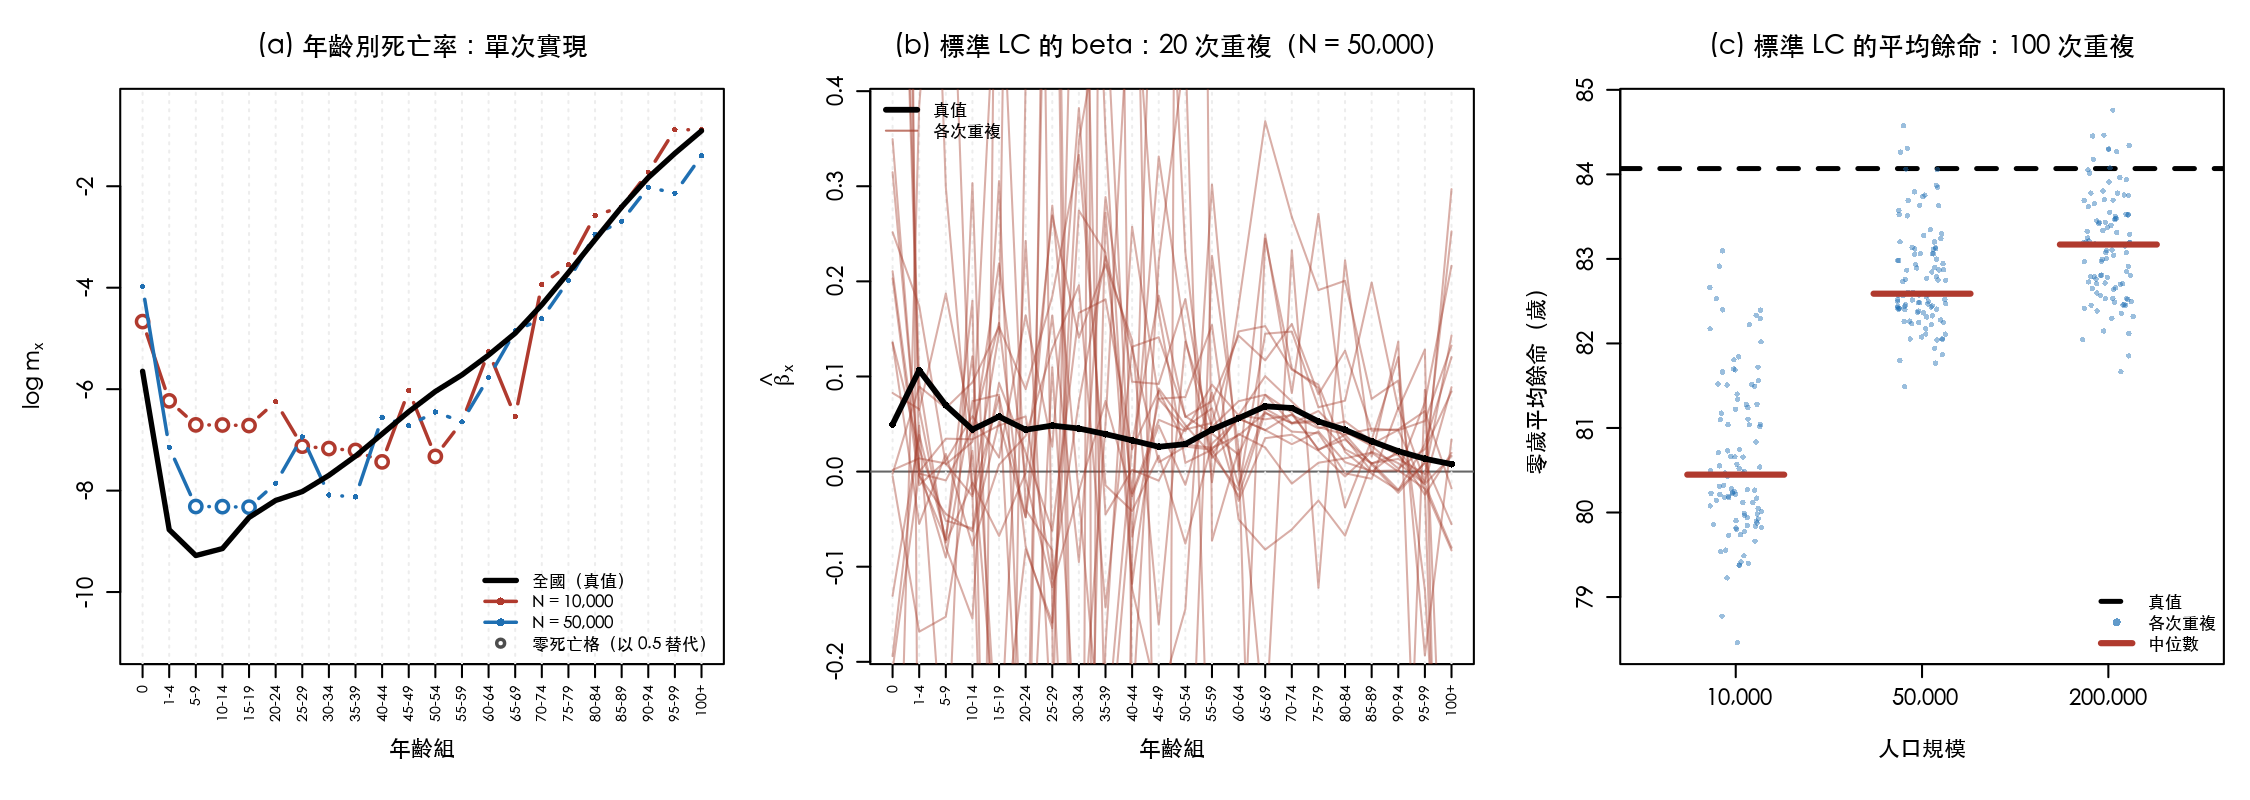
\includegraphics[width=\textwidth]{figT0_oscillation.png}
\caption{小人口下 Lee-Carter 估計的震盪與偏誤（臺灣女性，以全國配適為真值）}

{\footnotesize 註：(a) 單次實現的年齡別死亡率，空心點為零死亡格；(b) $\hat\beta_x$ 的 20 次重複；(c) 零歲平均餘命的 100 次重複，虛線為真值。}

\label{fig:osc}
\end{figure}

由圖~\ref{fig:osc}(a) 可以看到，人數一萬時 1 至 19 歲的各組幾乎全是
零死亡格（空心點），以 $0.5$ 替代後被擺在真值曲線之上約兩個對數單位；
人數五萬時情況緩解但仍有多格為零。
明顯之處在於這些點並不是隨機地散在真值兩側，而是一致偏高，
亦即震盪與偏誤在此是同一個機制的兩面。
圖~\ref{fig:osc}(b) 則顯示震盪傳到參數上的結果：$\hat\beta_x$ 描述各年齡
對時間趨勢的敏感度，其真值在幼年與 65 至 74 歲有兩個峰，
但 20 次重複的軌跡完全看不出這個形狀，甚至頻繁出現負值。
不明顯之處在 (c)：以配適末年的零歲平均餘命為例，
真值為 $84.07$ 歲；標準 Lee-Carter 的重複中位數在人數一萬、五萬、二十萬時
分別為 $80.45$、$82.59$、$83.17$ 歲，即系統性低估 $3.62$、$1.48$、$0.90$ 歲；
同時 $5$ 至 $95$ 百分位的全距為 $3.00$、$1.84$、$2.01$ 歲。
人數五萬時偏誤（$1.48$ 歲）與整個隨機全距（$1.84$ 歲）幾乎相同，
亦即把估計重複一百次所看到的全部變動，其幅度不過與一個看不見的系統性
偏移相當。考慮到我國縣市之間平均餘命的最大差距約為 $10$ 歲，
$1.48$ 歲的偏誤已足以使一個地區在排序上錯置數個名次。
簡言之，圖~\ref{fig:osc} 所呈現的是：若不處理偏誤，鄉鎮市區生命表所顯示的
地區差異將有相當部分是估計方法的產物，而非真實的健康差異。

此一偏誤的實務後果在於地區之間的比較。鄉鎮市區生命表的用途多為排序與資源
配置，而排序只需要各地區之間的相對位置正確；但偏誤的量隨人口規模而變，
人口較少的地區偏移較大，因此各地區的相對位置會被系統性地改變，
而該改變來自估計方法而非真實的健康差異。
加大人口規模並非可行的補救，蓋因鄉鎮市區的規模由行政區劃決定；
延長觀測期間亦不可行，理由見第\ref{subsec:consistency}。

\label{subsec:problem}%
圖~\ref{fig:osc} 的三格指出兩個性質不同的問題；兩者必須分開處理。
其一是\textbf{震盪}：人數少時年齡別死亡率的觀測值劇烈跳動，
零死亡格頻繁出現，估計量在重複抽樣下的變異大。
其二是\textbf{有方向的偏誤}：Lee-Carter 的年齡參數在人數減少時會朝同一方向偏移，
零歲平均餘命則一致低估。
蓋因震盪看得見而偏誤看不見，兩者的發現方式也不同：
震盪可由重複抽樣或加寬區間察覺，偏誤卻在所有樣本上朝同一方向偏移，
單看估計結果無從發現。既有的小人口研究多以重複抽樣觀察此一問題，
於是對震盪的刻畫遠比對偏誤的刻畫完整。

本文處理後者。這個選擇所依據的判斷是：既有文獻對偏誤的處理，
都停在「設法提高資料的訊息量」或「設法降低觀測的變異」這一層，
而未上溯至偏誤的生成環節。既有模擬一致顯示偏誤的方向是確定的，
而方向確定意味著它由估計程序中某一個特定步驟所產生，其量因此應可直接寫下。
第\ref{sec:lit}節將說明這一步之所以未被追究，
源自死亡率文獻處理對數尺度的方式是換掉它而不是去計算留在其上所付的代價；
而本文的切入點即在於把這筆代價算出來。

\label{subsec:design}%
本文的目的在把上述有方向的偏誤由一個須以模擬觀察的現象，轉為一個可以直接
計算的量，並據以設計校正。所循的路徑如下。標準 Lee-Carter 的估計是對
$\log\bigl(\max(D_{x,t},c_0)/E_{x,t}\bigr)$ 作最小平方，
在 $M$-估計的架構中即取平方損失的估計量；而 $M$-估計量要在真值處一致，
其估計方程在真值處的期望須為零，該期望在反應變數先經非線性轉換之後不再
自動為零。本文因此計算標準 Lee-Carter 的估計方程在真值處的期望，寫出其一般形式，
再檢視該形式在 Poisson、常態與過度離散三種分布下的具體樣貌。

此一路徑的兩項後果決定了全文的結構。偏誤的量既然可以寫出，
它就可以在配適之前算出，本文的第一條主軸是\textbf{診斷}：
標準 Lee-Carter 在某一組資料上會偏多少，由曝露數與一組粗略死亡率即可定出，
不需要模擬、真值或參考母體。偏誤的量既然可以算出，它也就可以扣除，
第二條主軸是\textbf{校正}：扣除的位置決定了年齡水準與年齡敏感度兩項改善
得以疊加的條件。兩條主軸的適用範圍不同，前者只依賴分布假設，
後者另依賴秩一雙線性結構，此一差別於第\ref{sec:disc}節一併交代。

\section{文獻回顧}\label{sec:lit}

標準 Lee-Carter 的第一步，亦即先取對數、再把零死亡格替換掉，
自 1992 年以來未曾更動。本節的回顧即以這一步為軸：以下四條線索看似分屬
死亡率、修勻、概似與穩健統計四個領域，實則都是對同一個步驟的回應，
而其中三條各自已經記載了這一步的問題。
死亡率文獻在 1993 年就注意到零死亡率使對數無定義，所給的兩種處理是
零權重與改用 Poisson；概似一側指出「加一個常數」正是預先修正在單樣本下的
形式，並已警告該作法使估計量不隨資料的彙總方式不變；
計量經濟一側把同一件事證成單位依賴。
未被處理的恰好是這三者都繞開的那一個組合，亦即\textbf{替代之後仍留在對數
尺度上}，而這正是標準 Lee-Carter 的作法。以下依序回顧四條線索，
並於各處指出它們彼此相接的位置。

\subsection{Lee-Carter 模型、其變體，與小人口下的參數偏誤}\label{subsec:lc}

最早把年齡與時間分離的雙線性死亡率模型由 \citet{lee1992} 提出，
其作法是以奇異值分解配適 $\log m_{x,t}=\alpha_x+\beta_x\kappa_t$，
再以時間序列模型外推 $\kappa_t$；由於形式簡單、參數可解釋、
且外推只需處理一個單變數序列，很快成為各國死亡率預測的基準模型，
亦為聯合國與多國統計機構所採用。

在應用的過程中，三項技術問題陸續被指出，而每一項都各自引出一條補救。
首先是配適末年與觀測值的系統性差距。\citet{leemiller2001} 以多國資料評估原始
作法的預測表現，發現第二階段重解 $\kappa_t$ 時若以總死亡數對齊，
配適末年的死亡率與觀測值仍有系統性差距，於是建議改為對齊當年的零歲平均
餘命，此即後續文獻所稱的 Lee--Miller 變體。
其次是誤差變異的設定。\citet{brouhns2002} 指出奇異值分解隱含各年齡的誤差
變異數相等，而死亡數為計數資料、其變異隨水準而變，兩者不符，
因此改以 Poisson 對數雙線性模型直接配適計數，
把估計由對數尺度的最小平方換為計數尺度的最大概似。
再者是 $\hat\beta_x$ 的不平滑。\citet{currie2004} 發現逐年齡估計的
$\hat\beta_x$ 在相鄰年齡之間劇烈起伏，而真實的年齡型態應為平滑，
因此把 \citet{eilers1996} 的懲罰 B-樣條引入死亡率配適；
\citet{delwarde2007} 則在 Poisson 對數概似上直接加差分懲罰，
使修勻與配適在同一個目標函數內完成。

上述補救本身又引出新的問題。\citet{djeundje2010} 發現以年齡與年份分類的
死亡資料常有過度離散，其變異數大於均值，於是 Poisson 假設雖較常態為佳
卻仍不足，因此放寬為「變異數與均值成比例」的擬似概似設定。
值得在此先指出一段與本文直接相關的早期發展。
依 \citet[\S4.3]{basellini2023} 的記載，Wilmoth（1993）即已指出奇異值分解
所隱含的 Gauss 架構不適用於人類死亡率，並提出兩種替代作法：
其一是以死亡數為權重的加權奇異值分解，該作法同時\textbf{以零權重迴避了零
死亡率使對數無定義的困難}；其二是改採 Poisson 假設，此即
\citet{brouhns2002} 之後所循的路。
換言之，死亡率文獻對零格的兩種既有處理是\textbf{丟棄該格}與\textbf{離開
對數尺度}，而非以某個正值替代；而第一種作法所用的權重，
正是本文第\ref{sec:weight}所推導之資訊加權的前身。
\citet{currie2013} 進一步把這一類帶約束與懲罰的廣義線性模型寫成一般的
計算框架，使各種變體可在同一套程式內實作。
模型本身的擴充亦同時進行，\citet{renshaw2003} 加入年齡別的增強項，
\citet{camarda2021} 則把修勻、分解與預測整合於同一套平滑架構。
\citet{rabbi2021} 另指出修勻的選擇會改動預測所隱含的壽命離散度，
因此修勻並非只影響參數的外觀。

這些變體隨後被系統地評比。\citet{booth2006} 以多國資料比較各變體的預測
表現，\citet{shang2011} 進一步把十種主成分型作法並列，
同時比較點預測與區間預測，指出各變體之間的差異在區間上比在點上更明顯。
\citet{hunt2020} 則系統刻畫了年齡--時期類模型的識別性問題，
指出若不施加額外約束，參數的個別數值並無唯一解。
Lee-Carter 第一階段的奇異值分解在函數型資料的語彙中即為主成分分析：\citet{hyndman2007} 以穩健的函數型主成分分析處理戰爭與疫情
等離群年份，\citet{hormann2015} 則把主成分推廣到容許時間相依的動態版本。
\citet{basellini2023} 在模型提出三十年後做了整體回顧，
並把小人口列為尚未解決的課題之一。

小人口下 Lee-Carter 估計的核心現象是年齡參數的低估。既有文獻的共同發現是，
人數減少時 $\hat\alpha_x$ 與 $\hat\beta_x$ 會朝同一方向偏移，
而該偏移在重複抽樣中方向一致，於是屬偏誤而非變異。
\citet{chen2017} 最早把人口規模獨立為研究的對象，以英格蘭與威爾斯的資料
指出隨機死亡率模型的參數不確定性與人口規模直接相關，在小人口下不可忽略，
並區分了來自母體規模的抽樣變異與來自模型的參數變異。
\citet{wang2018} 以模擬給出該偏移的量級，指出 Lee-Carter 的年齡參數
$\hat\alpha_x$ 與 $\hat\beta_x$ 在人數減少時同向偏移，
且在人數二十萬以下時特別明顯。
\citet[Figure 1]{yue2019} 把兩個參數分開，發現 $\hat\alpha_x$ 的偏誤恆為正
且量級遠大於 $\hat\beta_x$；後者在人數超過十萬時平均而言已接近零。

國內的研究亦指向同一現象，且其規模設定更貼近鄉鎮市區。
陳政勳與余清祥（2010）探討臺北市、雲嘉兩縣與澎湖縣的小區域人口推估，
王信忠等（2012）以區塊拔靴法發現南港區（單一性別約五萬人）的平均餘命
預測區間寬度超過十歲，王信忠等（2017）編製規模與鄉鎮市區相當的臺灣原住民
生命表，余清祥等（2021）以年輪變動比處理小區域人口推估，
余清祥等（2025）則改以標準化死亡率與平均餘命的線性關係繞過生命表的編算。

這一支至此已完成現象的提出、量化與分解，而它所留下的缺口在於\textbf{描述
的形式}：上述各文對偏誤的陳述一律是模擬所得的現象，
未見有研究上溯至該偏誤的生成環節，亦未見其量的解析形式。
缺乏解析形式的直接後果是，使用者無從在配適之前判斷某一組資料會偏多少，
只能逐案以模擬估計；而模擬須先指定真值，這在實際的小區域應用中並不可得。
以下兩小節回顧文獻對此的兩類應對：一類設法補進外部資訊，
另一類設法改動估計的機制。

\subsection{多母體、參考母體與修勻}\label{sec:ref}

第一類應對的共同想法是：既然困難出在資料的訊息量不足，
就從目標區域之外補進訊息。補進的方式有兩種，而兩種都以「外部資訊與目標
區域足夠相似」為前提。

這兩種方式在文獻中已被認定為同一個想法的不同應用。
\citet{wang2018} 明言，以增加母體規模或參照其他母體來改善死亡率估計
「並非保險業所獨有，信賴度與死亡率修勻是採同一想法的另兩個著名應用」，
因此修勻與信賴度的方法可用於改善小人口下的模型配適；
\citet{ahcan2014} 亦自稱其作法是「一種信賴度的取徑」，
以鄰近母體的平均死亡率與目標母體的原始資料混合。
這一點使本小節的修勻與第\ref{subsec:mest}末的信賴度標準成為同一條線索的
兩端，而不是兩個互不相干的領域。

其一是把母體合併。\citet{lilee2005} 合併死亡改善型態相近的多個母體，
以共同因子描述其共同趨勢；\citet{jarner2011} 以大型參考母體配適共同趨勢
而只讓小母體估計其偏離，此即 SAINT 模型；
\citet{ahcan2014} 把小母體的死亡資料與其他母體的資料混合，
以處理觀測序列中的劇烈隨機波動；
\citet{wang2018} 則建議聚合目標母體十至二十年的歷史資料。

其二是修勻。\citet{lee2003} 提出 partial SMR，以標準化死亡比把小區域的
年齡別死亡率朝參考母體收縮；\citet{yue2019} 把 partial SMR 與
\citet{whittaker1923} 修勻接在 Lee-Carter 之前或之後，比較兩種接法的表現。
修勻這一條須展開，蓋因它與本文處理的是同一個病灶的兩種解法。
\citet{lee2003} 提出 partial SMR 的動機，與本文的動機幾乎相同：
其摘要列出兩項困難，即小人口的年齡別率估計不穩定、
年齡曲線含過多隨機變異，以及「當分子含零計數時無法取對數」，
後者即零死亡格的困難。所選的解法是引入一個年齡曲線相近的標準母體，
以標準化死亡比為中心把觀測朝該母體收縮。

記 $d_x$ 為目標小區域 $x$ 歲組的死亡數觀測值、$P_x$ 為其曝露數、
$m^R_x$ 為參考母體同年齡組的中央死亡率，則期望死亡數為 $e_x=P_x m^R_x$，
標準化死亡比為 $\mathrm{SMR}=\sum_x d_x\big/\sum_x e_x$。
修勻後的死亡率定義為
\begin{equation}\label{eq:psmr}
v_x \;=\; m^R_x\,\exp\!\left(
\frac{d_x\hat h^2\log(d_x/e_x)+\bigl(1-d_x/\textstyle\sum_x d_x\bigr)\log \mathrm{SMR}}
     {d_x\hat h^2+\bigl(1-d_x/\textstyle\sum_x d_x\bigr)}\right),
\end{equation}
其中 $\hat h^2=\max\bigl\{[\sum_x(d_x-e_x\mathrm{SMR})^2-\sum_x d_x]
\big/[\mathrm{SMR}^2\sum_x e_x^2],\,0\bigr\}$ 度量兩個母體之間年齡別死亡率
比值的異質性。$\hat h^2$ 的構造是把觀測與期望死亡數的平方差減去 Poisson
本身的變異，蓋因比值的異質性必然伴隨超出 Poisson 所能解釋的變異，
此即上式分子中減去 $\sum_x d_x$ 的來由。
式~\eqref{eq:psmr} 是觀測的對數死亡比 $\log(d_x/e_x)$ 與整體
$\log\mathrm{SMR}$ 的加權平均，其權重的設計使死亡數愈少的年齡愈倚賴參考母體。
此一形式與保險的信賴度估計同型 \citep{klugman2012}，
也與 \citet{kimeldorf1967} 的貝氏修勻同屬一類。

式~\eqref{eq:psmr} 有兩項性質決定了該法的適用範圍。
首先，$d_x=0$ 時觀測端的權重為零，修勻值退化為 $\mathrm{SMR}\cdot m^R_x$，
恆為正。參考母體修勻因此根本不需要替代值，
零格的困難在這條路上是以外部資訊解決的，而非以慣例解決的。
\citet{lee2003} 據此主張該法「漸近不偏且不存在零計數問題」。
其次，$\hat h^2=0$ 時所有年齡都完全採用 $\mathrm{SMR}\cdot m^R_x$，
亦即整條年齡曲線的\textbf{形狀}來自參考母體，只有水準由目標區域決定。
這說明該法的表現必然取決於兩個母體的形狀是否相近，
而這一點與原文「標準母體的選擇不關鍵」的主張存在張力。

\citet{yue2019} 正是以此為主題，另考慮 \citet{whittaker1923} 修勻的
比值版本，即先取 $s_x=(d_x/P_x)/m^R_x$，再以
$\min_r \sum_x w_x(r_x-s_x)^2+h\sum_x(\Delta^z r_x)^2$ 求修勻後的比值，
取 $w_x$ 為曝露數、$h$ 為各年齡曝露數的平均。
所設計的七種比值情境為 $s_x$ 固定於 $0.8$、$1.0$、$1.2$，以及隨年齡遞增、
遞減、V 型與倒 V 型，以 100,000 人對 2,000,000 人的模擬比較，
結論是：在前三種情境下 partial SMR 的平均絕對百分比誤差明顯最小
（約 $12\%$，不修勻為 $25$--$29\%$），但在遞增情境下惡化至 $47.65\%$；
Whittaker 比值修勻則在七種情境下都穩定在 $14$--$19\%$。
並指出若把遞增情境的比值範圍由 $0.5$--$1.5$ 縮為 $(1-a)$--$(1+a)$，
則 $a\le 0.4$ 時 partial SMR 仍較佳。
綜上所述，這一支的發展是：提出者以零格無法取對數為動機、以外部母體為解法，
並主張對該母體的選擇不敏感；後續的檢驗則界定了該主張成立的範圍。

合併母體與修勻兩條支線近年已被接在一起。\citet{pitt2018} 在廣義線性模型的
框架內同時施加 P-樣條修勻與線性約束，並以共同因子聯合配適兩性的死亡率，
亦即把「換成 Poisson」、「加修勻」與「借用另一個母體」三項補救放進同一個
目標函數求解，其結果在樣本外的預測誤差上優於逐項施加者。
這一條因此是第一類應對發展的終點：外部資訊能借的都借了。

這一類作法所留下的缺口不在理論前提而在\textbf{資料的可得性}。
它要求分析者先有一個型態相近的參考母體，而在鄉鎮市區的應用中，
自然的參考母體是全國或鄰近地區，但臺灣縣市之間零歲平均餘命的最大差距
超過十歲 \citep{yue2019}，鄰近地區的社經組成亦常有明顯差異，
\citet{wangyue2026} 於是改以分群尋找合適的參考母體，
但同時指出相鄰地區的社經組成常有明顯差異，
使參考母體的選取本身成為一個待解的課題。
換言之，這條路把問題由「如何從少量資料估計」轉為「如何判斷參考母體是否
可用」；後者無法由目標區域自己的資料回答。
下一小節所回顧的第二類應對即不需要外部母體，其代價則轉移到分配假設上。

\subsection{對數轉換、零格替代與有限樣本偏誤的修正}\label{sec:logzero}\label{sec:biasred}

第二類應對不補進資料，而是改動估計的機制。改動的位置有兩處：
一是把估計所在的尺度換掉，二是把估計量本身改掉。
本小節依序回顧兩者，蓋因此處的推導正落在這兩者之間。

死亡率文獻的作法屬前者，亦即\textbf{換掉對數尺度}。
\citet{brouhns2002} 以 Poisson 對數雙線性模型取代 Lee-Carter 原始的對數尺度
最小平方，\citet{delwarde2007} 在 Poisson 概似上加懲罰以平滑 $\beta_x$，
\citet{djeundje2010} 進一步放寬為容許過度離散的擬似概似，
\citet{currie2013} 則把這類受限的廣義線性模型寫成一般的計算框架。
這條路之所以可行，是因為計數尺度上零並非奇點，零死亡格不需要任何替代值。
而留在對數尺度上加常數的作法，在概似一側已被明確地勸阻。
\citet[\S6.2]{kosmidis2014} 以「對一般情形中加常數的一項警告」為標題，
指出此類作法雖自 \citet{haldane1956} 以來成為稀疏計數的標準實務，
卻有一項結構性的缺點：\textbf{加項是常數，所得的估計量因而不隨資料的表達
方式（彙總或未彙總）而不變}，而這一項不變性是最大概似估計量本來具備的；
該文並以累積連結模型舉例，顯示對同一筆資料的兩種表達加上同一個常數，
所得的係數估計可相差甚大。

留在對數尺度上所付的代價，則在統計學與計量經濟學中有其獨立且完整的發展，
而該發展與死亡率文獻幾乎互不引用。以某個正值替代零、再取對數，
最早出現在比率的對數估計。\citet{haldane1956} 指出以對數勝算比估計時，
若某格為零則估計量不存在，提議在每一格加上 $1/2$；
\citet{anscombe1956} 在同一年由變異數穩定化的角度得到類似的建議。
兩者的動機都是\textbf{使估計量存在}，而非減少偏誤。
這個加項後來在偏誤修正的文獻中取得了明確的身分。
\citet[\S3.3]{firth1993} 指出，在單樣本的二項模型下，其預先修正所給的
估計量恰為 $\log\{(y+\tfrac12)/(m-y+\tfrac12)\}$，
亦即\textbf{對資料加二分之一之後的最大概似估計}，並明白把它認作
\citet{haldane1956} 與 \citet{anscombe1956} 所提之「降偏誤的經驗 logit」。
換言之，「加二分之一」不是一個權宜的慣例，
而是預先修正在單樣本情形下的特例。
\citet{gart1967} 隨後系統比較了各種加項對偏誤與變異數的影響，
指出加項的大小會改變估計量本身，而不只是處理零的技術細節；
\citet{gart1967} 因此是文獻中第一次明確指出替代值本身即影響估計結果的研究，
但其設定是二項比例，而非計數資料取對數後再作雙線性配適。

轉換本身所造成的偏誤則在迴歸的脈絡中被處理。
\citet{duan1983} 指出以 $\log y$ 為反應變數配適後，把配適值取指數回推並不會
得到 $y$ 的條件期望，差額取決於誤差的分布，並提出不需指定分布的 smearing
估計量加以修正。\citet{santossilva2006} 在國際貿易的重力模型中把這一點推到
更強的結論：在異質變異之下，對數線性模型的係數估計本身即不一致，
建議改以 Poisson 擬似最大概似直接在原尺度上配適。
這兩篇的共同訊息是：取對數之後的估計量，其偏誤由誤差的分布決定，
而不是一個可以忽略的高階項。

這條線最近的發展把問題的嚴重性提到更高一層。
\citet{chenroth2024} 處理的是反應變數可能為零時所採的各種「類對數」轉換，
例如 $\log(1+y)$ 與反雙曲正弦。所證明的是此類轉換下的平均處理效果並不能
解讀為近似的百分比效果，蓋因它依賴 $y$ 的\textbf{單位}：
只要在取轉換之前先把 $y$ 的單位重新尺度化，就可以得到任意量級的效果估計。
進一步的三難結果是，當反應變數可以為零時，
不存在一個同時是個體效果之平均、單位不變、且可點識別的參數。
其所建議的替代作法之一，正是回到水準尺度並以 Poisson 迴歸表達百分比效果。
\citet{mullahy2024} 由另一個角度得到相容的結論：此類轉換把零與正值分開，
使所估得的參數與一個經過尺度調整的線性機率模型相關，
而回推後的邊際效果與彈性對轉換中的形狀參數敏感，
其量級介於未轉換的最小平方與該線性機率模型之間；
於是建議不要轉換反應變數，改採兩部分模型或未轉換的迴歸。
\citet{chenroth2024} 所指出的單位依賴，在 Lee-Carter 的設定下所對應的即是
零格替代值的選擇：替代值與死亡數的尺度是相對的，
改變它等價於在取對數之前改變反應變數的單位，
因此「可以得到任意量級的效果」這個結論在小人口死亡率上即表現為
年齡水準參數的偏誤隨替代值而變。
\citet[\S6.2]{kosmidis2014} 的「不隨資料的表達方式而不變」與
\citet{chenroth2024} 的「依賴反應變數的單位」，在結構上是同一項性質：
兩者都指出一個固定的加項使估計結果取決於分析者所選的尺度，
而該尺度不由資料決定。前者由概似的不變性切入、後者由識別性切入，
兩個文獻互不引用，結論卻一致。
這個結論也與死亡率文獻「換掉對數尺度」的選擇方向相同。

改動的第二個位置是\textbf{把估計量本身改掉}。就小樣本估計而言，
把估計量的期望拉回真值的作法分為兩種：先取得估計值再扣除其偏誤的事後修正
（Corrective Approach），以及修改估計方程使估計值自身即為降偏誤的預先修正
（Preventive Approach）；
兩者皆始於概似理論內部，以下依其發展順序回顧。
\citet{bartlett1937} 先處理概似比統計量的分布，指出其與漸近卡方分布的
$O(n^{-1})$ 落差可由一個乘數修正吸收；\citet{bartlett1953} 進一步給出最大
概似估計量 $O(n^{-1})$ 偏誤的展開。\citet{coxsnell1968} 把它寫成一般的形式，
此即事後修正：先取得最大概似估計值，再扣除其偏誤的估計。
這條線的應用隨後展開，\citet{cordeiro1991} 把該修正寫成廣義線性模型中
可由一次加權最小平方求得的形式，使其在實務上可行；
並指出對邏吉斯迴歸而言，偏誤向量幾乎與係數向量平行，
因此修正在方向上近似一個收縮。

問題則由 \citet{firth1993} 指出：事後修正必須先有有限的最大概似估計值，
而 \citet{albert1984} 早已刻畫了完全分離使該估計值發散的情形，
在這種情形下事後修正無從施加。小人口的死亡資料恰好容易落入該情形，
蓋因某個年齡若各年皆無死亡，Poisson 對數概似對該年齡的最大值即在負無窮處。
\citet{firth1993} 提出預先修正，把偏誤的首項移到分數函數上，
等價於在概似上乘一個 Jeffreys 型的懲罰，如此估計值恆為有限
（該文的推導另有勘誤，見 \citealp{firth1995}）。
該作法所修正的是 $O(n^{-1})$ 的首階偏誤，於是修正後的估計量仍帶有高階的偏誤，
而非期望恰等於真值。

此一作法後續被廣泛接續使用，其推廣的方向涵蓋了指數族的非線性模型。
\citet{kosmidis2009} 把它擴及指數族非線性模型，使其適用範圍涵蓋 Lee-Carter
這類雙線性的設定；\citet{kosmidis2011} 以 Poisson 對數線性模型的等價表示
處理多項邏吉斯迴歸；\citet{kosmidis2014} 處理累積連結模型。
其中 \citet{kosmidis2010} 的結果最為一般，給出一個通用的疊代演算法，
只要某個模型的最大概似估計量的首階偏誤已經導出，即可據以計算其降偏誤估計，
並明言該演算法可視為\textbf{一連串的疊代偏誤修正}。
該演算法有兩項性質。首先，它把事後修正與預先修正統一為同一個
演算法的兩個端點，因此「算出偏誤再扣除、並反覆至收斂」這個作法在方法論上
已有先例。其次，它所要求的輸入是「偏誤的可寫出形式」而非「概似的存在」，
因此偏誤只要能由反應變數的邊際分布算得，該演算法即可施加。

後續發現的新問題有兩項。期望不偏並不蘊含中位數不偏，且前者不具再參數化
不變性：一個在某個參數化下期望不偏的估計量，經非線性重新參數化後即不再如此。
\citet{kennepagui2017} 於是提出中位數偏誤修正，同樣以修改分數方程的方式
達成，所得估計量在保持興趣參數的再參數化下不變、且為三階中位數不偏，
並與 \citet{firth1993} 同樣可避免無限估計值；
\citet{kennepagui2020} 把該作法用於 Cox 迴歸的單調概似情形。
修正的量另隨模型而異，目前並無涵蓋所有模型的通用公式；
\citet{cordeiro1991} 在結語中即以此說明每一類模型都須個別推導的原因，
而這條線至今仍在逐一擴張，例如 \citet{sossa2026} 把 Cox--Snell 修正推到
均值與離散度同時變動的異質變異非線性模型。

\citet{breslow1995} 的結果與本問題的情形最為接近：其處理帶單一變異成分的
廣義線性混合模型，推導三種近似估計量（含懲罰擬似概似）的漸近偏誤，
發現一階估計量對變異成分的估計有嚴重偏誤，
而該偏誤的量\textbf{由變異成分的大小決定，不是由樣本數決定}；
並給出易算的修正因子；\citet{linbreslow1996} 把結果推廣到多個變異成分。
此一分支確立了一個先例：偏誤修正的原理不限於 $O(n^{-1})$ 的漸近項，
而可施加於任何可寫出其偏誤的近似，且該偏誤不必隨樣本數消失。
偏誤修正本身也早已進入死亡率文獻，只是施加的對象不同：
\citet[\S4]{djeundje2010} 在處理過度離散時，即為離散參數的估計導出一個
修正，並把所得的流程逕稱為「偏誤修正的方案」。
亦即死亡率文獻熟悉偏誤修正這個工具，而把它用在離散參數上，
未用在年齡參數上。

這一分支同時把本小節的兩處改動接了起來。\citet{lin1999} 以平滑樣條處理廣義
加法混合模型的推論，\citet{kauermann2009} 給出廣義懲罰樣條平滑的漸近結果，
\citet{xiao2020} 則處理函數型資料的懲罰樣條；
而本小節開頭所述死亡率修勻的一路
（\citealp{currie2004}；\citealp{delwarde2007}；\citealp{currie2013}）
在統計理論上即屬這一類模型。亦即死亡率文獻為了平滑而引入的工具，
其自身的文獻早已記載其近似概似會產生不隨樣本數消失的偏誤；
死亡率文獻引入這些工具時關注的是平滑度，並未援引這一側的偏誤結果。

上述結果都建立在「有一個可寫下的概似」之上，
而標準 Lee-Carter 先取對數再作最小平方，其目標函數本就不是任何分配的對數
概似，因此其結果無法直接施加於它。缺口因此相當具體：
標準 Lee-Carter 的實作至今仍以對數尺度的奇異值分解為主，
\citet{lee1992} 的原始作法如此，\citet{yue2019} 在小人口的研究中所修改的
對象亦是該作法；而只要使用這個作法，零格就必須以某個正值替代。
就本文所查，該替代值的選擇對 Lee-Carter 參數估計的影響尚未被量化，
$0.5$ 這個慣例在死亡率文獻中亦未見其出處的討論。
缺口因此不在於沒有人注意到這一步，而在於\textbf{三條線索各自繞開了它}：
死亡率文獻以零權重或 Poisson 迴避，概似一側勸阻加常數而未處理加了之後的
後果，計量經濟一側建議不要轉換反應變數。
在本文所查的死亡率文獻中，無一引用 \citet{haldane1956} 以來的加項文獻或
\citet{duan1983} 以來的轉換偏誤文獻；
\citet{haldane1956} 以來的「加一個常數」、\citet{duan1983} 以來的
「轉換造成偏誤」與 \citet{chenroth2024} 的「單位依賴」三條線索，
至今未被接到小人口死亡率的設定上。

\subsection{$M$-估計、混合表示、損失與懲罰的分類，與信賴度標準}\label{subsec:mest}\label{subsec:mix}\label{subsec:mq}\label{subsec:cred}

上一小節的缺口可以一句話寫定：標準 Lee-Carter 的目標函數不是任何分配的
對數概似，於是以概似為前提的偏誤修正無從施加。但它仍然是某個目標函數的
極小值；這一點足以使它落入一個更一般的框架。本小節回顧該框架，
依序為 $M$-估計與 Fisher 一致性、誤差分布的混合表示、
損失與懲罰的一般分類，以及本文結果所要接上的精算實務標準。

\citet{huber1964} 提出 $M$-估計量，把最大概似的想法推廣為「某個目標函數的
極小值」或等價地「某個估計方程的解」：$\hat\theta$ 解
$\sum_i\psi(y_i;\theta)=0$，其中 $\psi$ 不必是對數概似的導數。
其動機是位置參數的穩健估計，設定為 $\varepsilon$-污染（絕大多數觀測
來自模型、少數來自別處），目標在於使少數觀測無法主導估計。
此一概念隨後被量化：\citet{hampel1974} 以影響函數刻畫單一觀測的影響力，
\citet{donoho1983} 以崩潰點（Breakdown Point）刻畫可承受的污染比例上限，
\citet{huber2009} 為該領域的標準專著；而穩健性所付的代價為效率，
例如中位數在常態下相對於樣本平均的效率僅 $2/\pi\approx0.64$。
本文推導時所依循的記號取自 \citet[第 1 章]{zoubir2018}：該章把估計量寫成
作用在經驗分布上的泛函 $\hat\theta_N=T(F_N)$（該書式 1.30），
以 $T(F)$ 與真值之差定義漸近偏誤，並於 §1.2、§1.3.1 與 §1.3.2 分別給出
$M$-估計量作為估計方程之解的定義、影響函數與崩潰點。
本文的核心推導並未直接引用該書或以下各書中的現成定理，所借用的是框架與記號。
在應用上，$M$-估計已是訊號處理、電力系統狀態估計與電腦視覺的常規工具
\citep{zoubir2018}，其場景的共同特徵是觀測數遠大於參數數、
且離群值確實是少數。在死亡率文獻中，\citet{santolino2020} 把分位數迴歸
引入 Lee-Carter 模型，屬同一個框架下改動損失函數的作法。

$M$-估計的另一條發展線把「估計方程」本身當成建模的對象，而不必先寫下
概似。\citet{liang1986} 的廣義估計方程即屬此類，
其以工作相關矩陣處理相依資料而不指定聯合分布，在縱貫資料分析中已成常規；
\citet{merlo2022} 進一步把廣義估計方程推廣到帶 Huber 損失的 M-分位數。
這條線近年在因果推論中被推到一般的原則：\citet{chernozhukov2018} 要求所用的
估計方程在擾動參數的真值處對該擾動的一階變動不敏感，
並以樣本切分使該性質在高維擾動下仍成立，其所稱的去偏即是把估計方程本身
重新構造到期望為零。這條線確立了一個看法：一個估計量的性質，
可以完全由其估計方程的期望與變異數讀出，
而不必訴諸該估計量是否為某個概似的最大值。

$M$-估計理論中另有一項比穩健性更為基本的性質，
即\textbf{Fisher 一致性}（Fisher Consistency）。
一個 $M$-估計量要在真值 $\theta_0$ 處一致，
必要條件是估計方程在真值處的期望為零，
$\Ex_{\theta_0}[\psi(Y;\theta_0)]=0$；否則 $\hat\theta$ 收斂到的是
使該期望為零的另一個點，與 $\theta_0$ 相差一個不隨樣本數消失的量。
此一條件在教科書中通常一行帶過，因為對最大概似而言它自動成立
（分數函數的期望為零），對最小平方而言只要誤差期望為零即成立。
但它之所以自動成立，前提是損失函數作用在未經轉換的反應變數上；
一旦反應變數先經過非線性轉換，$\Ex[\psi]=0$ 就不再是自動的，
而古典文獻對此一情形並未展開。

這一支的標準設定與小人口 Lee-Carter 之間另有幾處差異。
古典 $M$-估計文獻關心的是 $\psi$ 有界所帶來的穩健性，
而小人口 Lee-Carter 所涉的是 $\psi$ 的\textbf{期望}是否為零，
兩者是不同的問題：平方損失的 $\psi(u)=u$ 完全不穩健，
但若 $\Ex[u]=0$ 它仍是一致的；反之一個很穩健的 $\psi$ 若 $\Ex[\psi]\ne0$
則仍不一致。其次，古典設定的觀測數遠大於參數數，而 Lee-Carter 模型每個
$\alpha_x$ 只有 $T$ 個觀測、每個 $\kappa_t$ 只有 $A$ 個，兩者皆為數十的量級。
再者，古典設定的污染比例未知，而零格替代所造成的污染比例則為已知，
見下文。另有一項結構上的差異。古典 $M$-估計的參數進入模型的方式是線性的
（$x_i^{\top}\theta$），而 Lee-Carter 的 $\alpha_x+\beta_x\kappa_t$ 對
$(\beta,\kappa)$ 是\textbf{雙線性}的，識別須靠兩個約束；
這使 $\hat\beta$ 與 $\hat\kappa$ 的漸近理論複雜得多；而年齡水準參數
$\hat\alpha_x$ 不受此影響，它在雙線性部分被估計之前即已由列平均定出，
因此可以完全在單變數 $M$-估計的框架內分析。

污染比例已知這一點，須由混合模型的表示法讀出。有限混合模型把觀測的分布
寫成若干成分分布的加權和，$f(y)=\sum_{j}\pi_j f_j(y)$。
其發展脈絡自 \citet{pearson1894} 以動差法分解螃蟹前額寬的雙峰分布起，
長期受限於計算；\citet{dempster1977} 的 EM 演算法使最大概似估計成為可行，
此後混合模型成為模型式分群的標準工具，\citet{mclachlan2000} 與
\citet{yao2024} 為前後兩代專著，後者涵蓋半參數推廣、穩健建模、
標籤交換與高維情形。本文所借用的即 \citet[§1.2]{yao2024} 的有限混合寫法，
而該書 §1.3 的識別性與 §1.4、§1.5 的最大概似與 EM 演算法皆以各成分有密度
為前提。在應用上，混合模型用於天文、基因體、經濟與金融等領域的異質資料；
在小區域估計中，\citet{delsarto2019} 以 M-分位數迴歸的有限混合處理未觀測
異質性，\citet{denicolo2023} 以 Beta 混合估計地區的不均度指標。

與計數資料最相關的一支是零膨脹模型。\citet{lambert1992} 的零膨脹 Poisson
迴歸把觀測寫成「一個零處的點質量」與「一個 Poisson」的兩成分混合，用以處理
製造業瑕疵計數中零的個數遠多於 Poisson 所能解釋者。此一形式與零格替代所
造成的混合極為相似，兩者的差別須先釐清。零膨脹模型所處理的是\textbf{結構上
多出來的零}，亦即資料生成機制本身含有一個「必然為零」的狀態，
因此零的個數超過 Poisson 的預期。零格替代所造成的混合\textbf{不是}零膨脹：
死亡數就是純粹的 Poisson，零的個數恰如其機率所預期，沒有任何多餘；
該混合是替代規則在取對數之後的變數上造出來的，因為 $\log 0=-\infty$
不可用，分析者必須把所有零格對應到同一個值，
於是轉換後的變數才出現一個點質量。亦即零膨脹模型的混合來自
\textbf{資料}，零格替代的混合來自\textbf{分析步驟}。
這個差別有實質的性質：零膨脹模型須估計膨脹比例，而零格替代的混合權重由
分布本身給定，無須估計；反之零膨脹模型可以不取對數而直接配適，
零格替代的困難則完全來自取對數這個步驟。

混合模型與穩健統計的連結早已建立：Huber 的 $\varepsilon$-污染模型
$(1-\varepsilon)F+\varepsilon H$ 就是一個兩成分混合。但兩個文獻的處理方式
相反。混合模型把 $\pi_j$ 與 $f_j$ 都當成待估的參數，以 EM 求解；
穩健統計則把 $\varepsilon$ 與 $H$ 當成未知的滋擾，設計對其不敏感的估計量。
穩健估計量之所以必須付出效率代價，正是因為 $\varepsilon$ 未知：
它必須針對最壞的情形設計。
這一支與小人口 Lee-Carter 之間的差異正在此處；該差異有一半是有利的。
零格替代使每一格的觀測成為一個兩成分混合；其混合權重是\textbf{已知的}，
它就是死亡數為零的機率，拿到資料即可估計；
既然如此，既不必以 EM 去估它，也不必為不知道它而承擔該項效率損失。
另一半則不利：該混合的其中一個成分是\textbf{退化的}（一個點質量），
而有限混合理論通常假設各成分有密度，於是識別性、標籤交換等標準議題在此
不適用，EM 亦無從施加。
另有兩項性質由混合權重已知而來。其一，\citet{donoho1983} 的 $50\%$ 上界
可直接換算為期望死亡數的門檻，不必以模擬估計；其二，零格替代所造成的污染
比例在幼年組可超過七成，因此穩健統計「污染為少數」這個前提在小人口死亡資料上
並不成立。

最後一個可借用的結果是分類。把損失函數、權重與懲罰整合為同一個目標函數的
作法，在小區域估計中發展得最完整。
\citet{koenker1978} 以檢查函數 $\rho_\tau$ 取代平方損失，
使迴歸得以刻畫條件分位數；\citet{koenker2005} 為標準參考，
其應用場景包括勞動經濟學的薪資分布與兒童生長參考曲線
\citep{wei2006}，共同特徵是每個共變數水準上有大量觀測。
該書第 5 章（頁 151--172）給出加權的最適形式，其中定理 5.1 指出分位數迴歸的
權重應與所關心分位處的局部密度成比例，而非與觀測標準差的倒數成比例；
第 8 章（頁 250--292）另討論離散反應與高崩潰點的替代方案，
並說明離散反應使該書標準設定下的漸近結果不再適用的原因。
\citet{breckling1988} 指出，若把 Huber 損失乘上一個依殘差正負
而異的非對稱權重，即得一個由 $(\tau,c)$ 索引的損失函數族 M-分位數，
其兩個極限分別是檢查函數（$c\to0$）與非對稱最小平方
（$c\to\infty$，\citealp{newey1987}）。

M-分位數在小區域估計中受青睞的理由如下。
傳統的小區域估計以 \citet{fay1979} 的隨機效果模型為主，
須假設區域效果的分布（通常為常態），其均方誤差的估計則由
\citet{prasad1990} 給出；兩者的收縮量由變異成分決定而無須指定懲罰強度，
但其推導假設直接估計量不偏、僅帶抽樣噪音。
\citet{chambers2006} 指出 M-分位數可直接給出各區域
自己的迴歸係數而不必作此分布假設，因此對分布誤設較不敏感；
該法的應用多為家戶調查資料的地方層級所得與剝奪指標估計。
這條線近年持續擴張，涵蓋推論理論、懲罰化、多變量相依、離散標的與均方誤差
的估計（\citealp{bianchi2018}；\citealp{hu2021}；\citealp{ranalli2023}；
\citealp{merlo2022}；\citealp{dawber2022}；\citealp{bugallo2025}；
\citealp{bugallo2026}），其中 \citet{lahiri2023} 把巢式誤差迴歸推廣到同時
容許區域別係數與區域別變異成分的情形，與本文第\ref{subsec:future}所列的
後續工作直接相關；\citet{jiang2026} 為這一整支的近期專著。

與此平行的是正則化一脈，其想法在小區域估計之外獨立發展。
\citet{stein1956} 指出高維常態平均數的樣本平均不可容許，
\citet{james1961} 給出具體的收縮估計量，
\citet{hoerl1970} 的 Ridge 與 \citet{tibshirani1996} 的 LASSO 則把收縮
寫成在目標函數上加懲罰項，\citet{zou2005} 與 \citet{zou2006} 再加以擴充。
\citet{fay1979} 的經驗貝氏收縮即是同一想法的區域層級版本。
這一脈的懲罰強度通常以交叉驗證選定，其標準論述見 \citet{buhlmann2011} 與
\citet{hastie2015}。把穩健損失與懲罰接起來的整理見 \citet{zoubir2018} 第 3 章，
其中並給出迴歸係數與尺度的聯合懲罰式 $M$-估計。
綜合之，這一支的一般目標函數為
\begin{equation}\label{eq:general}
\min_{\theta}\ \sum_{i} w_i\,\rho_{\tau,c}(u_i(\theta))\;+\;\lambda P(\theta),
\end{equation}
其中含三項設定：損失形狀 $(\tau,c)$、權重 $w$、懲罰 $(\lambda,P)$。

這一支的標準設定與小人口 Lee-Carter 之間的差異亦有數處。
其應用場景是單位層級的調查資料，每個小區域有多個受訪單位；
而死亡率資料是聚合的計數，每格只有一個觀測。
其次，三項設定都需要調參（$\tau$、$c$、$\lambda$），
而死亡率資料既無真值、亦無法以交叉驗證選參，蓋因切分年齡--年份格會破壞
雙線性結構所依賴的跨格借力，被留置的格無法由其餘的格預測。
再者，這一脈的漸近理論均假設解釋變數已觀測，而 Lee-Carter 的 $\kappa_t$ 是
待估的潛在變數而非觀測值，於是上述理論不能直接套用。
至於式~\eqref{eq:general} 本身，它把標準 Lee-Carter 納為一個角落
（$\tau=0.5$、$c=\infty$、$w\equiv1$、$\lambda=0$），
因此可以用來辨認各種補救各自改動了其中哪一項設定：
第\ref{sec:ref}所回顧的修勻改動的是資料，而本小節所列的各種方法改動的是
損失形狀、權重或懲罰。

最後一項可借用的結果不是統計推導所依的理論，而是精算的實務標準，
亦即本文結果所要接上的判準。保險業判斷一組資料是否足以單獨用於費率計算，
其依循的即是信賴度理論。全信賴度標準把資料量換算為期望索賠次數，
並要求該次數高到使估計量的相對誤差以指定的機率落在指定的範圍內；
在 $k=5\%$、$p=90\%$ 的慣例下，該門檻約為 $1{,}082$ 件
（\citealp{klugman2012}，第 17 章）。部分信賴度則以該門檻的平方根比例在
目標資料與參考資料之間插值，其形式與第\ref{sec:ref}的 partial SMR 同型。
此一標準有一項性質決定了本文結果所能接上的位置：\textbf{它控制的是估計的變異，
而其推導假設估計量無偏}。全信賴度的計算只用到估計量的變異數與常態近似，
偏誤不出現在任何一條式子裡。這在索賠次數的設定下是合理的，
因為該處的估計量就是樣本平均；但在小人口 Lee-Carter 的設定下並不成立，
蓋因其估計量在零格存在時即非無偏，而偏誤的量與資料量的關係並不隨資料量
增加而自動可忽略。就本文所查，信賴度文獻中並無與全信賴度標準對應的
\textbf{偏誤}門檻，缺口即在此處。

\subsection{本文的安排}\label{sec:roadmap}

綜合上述各脈絡的回顧，本文擬建立小人口 Lee-Carter 偏誤的閉式，
並據以設計校正，全文因此分三部。

第一部處理\textbf{診斷}。第\ref{sec:method}節把標準 Lee-Carter 辨識為取平方損失的
$M$-估計量，計算其估計方程在真值處的期望，說明年齡參數無法達到 Fisher
一致性，並把該不一致寫成閉式；第\ref{sec:second2}節在同一框架下導出對數
尺度的變異數、估計方程的靈敏度、校正所付的變異數代價，以及相對於 Poisson
最大概似的效率；第\ref{sec:valid}節交代研究資料與模擬設定，
並以臺灣女性的死亡資料核對前兩節的各式；第\ref{sec:feas}節把前述各式所需的
輸入限縮為曝露數與一組粗略死亡率，據以構造一個事前的可行性檢定與分級，
並以我國 368 個鄉鎮市區的年齡結構實作。

第二部處理\textbf{校正}。第\ref{sec:corr}節把第一部所得的量代回估計流程，
分解參數偏誤的確定性與隨機成分，並推導加權的最適形式；
第\ref{sec:result}節為實證結果，依序比較整體指標、逐年齡的改善剖面、
平均餘命的偏誤與離散、與參考母體修勻法的對照、模型誤設下的穩健性，
以及兩項改善得以疊加的條件。

第三部為第\ref{sec:disc}節，陳述所提修正的限制與界限，並收束全文的結論。


\partline{一}{偏誤的刻畫與診斷}

\section{取對數與零格替代所造成的偏誤}\label{sec:method}

\subsection{模型、記號與標準 Lee-Carter 的估計}\label{subsec:notation}

本節先寫定記號與標準 Lee-Carter 的估計流程，作為全文的基準。
本文以標準 Lee-Carter 模型為基準模型（baseline），並以三類修正方法與之比較：
\citet{firth1993}的預先修正、本文由 $M$-估計導出的中心化修正，
以及 \citet{lee2003}與 \citet{yue2019}的參考母體修勻。
由於本文全部的論證都建立在「標準 Lee-Carter 的 $\hat\alpha_x$ 是如何定義的」
這一點上，以下的流程敘述力求與實作一致。

參照 \citet{lee1992}，令 $x=1,2,\dots,A$ 為年齡組、
$t=1,2,\dots,T$ 為年份，Lee-Carter 模型可以下式表達：
\begin{equation}\label{eq:lc}
\log m_{x,t}=\alpha_x+\beta_x\kappa_t,\qquad
\sum_x\beta_x=1,\quad \sum_t\kappa_t=0 .
\end{equation}
其中 $m_{x,t}$ 為 $x$ 歲組於 $t$ 年的中央死亡率；
$\alpha_x$ 為 $x$ 歲組的死亡水準，即該年齡組對數死亡率在觀測期間的平均；
$\beta_x$ 為 $x$ 歲組的年齡敏感度，刻畫該年齡組的對數死亡率對時間因子
變動一單位的反應幅度；$\kappa_t$ 為 $t$ 年的死亡改善因子，
刻畫全體年齡共同的時間趨勢。兩個約束用以固定參數的尺度與位置，
否則 $(\beta_x,\kappa_t)$ 可同乘與同除一個常數而不改變配適值。

觀測為死亡數 $D_{x,t}$ 與曝露數 $E_{x,t}$。本文設
\begin{equation}\label{eq:pois}
D_{x,t}\sim\text{Poisson}(\mu_{x,t}),\qquad \mu_{x,t}=E_{x,t}\,m_{x,t},
\end{equation}
各格獨立，此即 \citet{brouhns2002}所採的設定。
以下的推導反覆用到三個前提，為便於引用，編號如下：
\textbf{(A1)} 式~\eqref{eq:pois} 成立，亦即各格的死亡數為獨立的 Poisson；
\textbf{(A2)} 期望死亡數 $\mu_{x,t}$ 落在式~\eqref{eq:lc} 的秩一雙線性結構上；
\textbf{(A3)} 存在一組可代入的 $\hat\mu_{x,t}$。
第\ref{sec:method}節的 Proposition~\ref{prop:fisher} 與
Corollary~\ref{cor:alpha} 都不需要 (A1)，只需期望存在；
第\ref{sec:second2}節的二階量需要 (A1)；
第\ref{sec:corr}節的校正另需要 (A2) 與 (A3)。
$D_{x,t}=0$ 時 $\log(0/E)=-\infty$，於是實務上必以某正值 $c_0$ 替代。
在計數資料的對數轉換中，以 $1/2$ 作為替代值是長期的慣例，
其源頭可追溯至 \citet{haldane1956}與 \citet{anscombe1956}對對數勝算比的偏誤修正，
\citet{gart1967}則系統比較了各種加項的偏誤與變異數；
本文沿用此一慣例，取 $c_0=0.5$，並在第\ref{subsec:bprops}說明該選擇
對後續結論的影響。令
\begin{equation}\label{eq:ell}
\ell_{x,t}=\log\frac{\max(D_{x,t},\,c_0)}{E_{x,t}},\qquad
u_{x,t}(\theta)=\ell_{x,t}-\alpha_x-\beta_x\kappa_t .
\end{equation}

標準 Lee-Carter 的估計分兩階段。第一階段以兩個步驟依序求出三組參數：
先取各年齡的列平均作為年齡水準的估計，
再對扣除列平均後的殘差矩陣作奇異值分解，取第一組奇異向量作為
年齡敏感度與時間因子的估計，即
\begin{equation}\label{eq:svd}
\hat\alpha_x=\frac1T\sum_{t=1}^{T}\ell_{x,t},\qquad
\hat{\boldsymbol\beta},\hat{\boldsymbol\kappa}:\quad
\{\ell_{x,t}-\hat\alpha_x\}\ \text{的第一組奇異向量，再依兩個約束正規化} .
\end{equation}
須強調式~\eqref{eq:svd} 的順序：$\hat\alpha_x$ 在奇異值分解\textbf{之前}
即已定出，其值不因 $\hat\beta_x,\hat\kappa_t$ 如何正規化而改變。
這一點是第\ref{sec:joint}能把兩項改善疊加的全部理由，
而它在識別性的語言中有一個精確的位置。\citet{hunt2020} 指出式~\eqref{eq:lc}
有兩個不變變換，亦即 $(\alpha_x,\beta_x/a,a\kappa_t)$ 與
$(\alpha_x-b\beta_x,\beta_x,\kappa_t+b)$，前者使 $\beta$ 與 $\kappa$ 的尺度
不可識別、後者使 $\kappa$ 的位置不可識別，而 $\sum_x\beta_x=1$ 與
$\sum_t\kappa_t=0$ 這兩個約束恰好各固定其中一個自由度。
$\alpha_x$ 在前一個變換下不動，只在後一個變換下隨 $b$ 平移；
而取列平均即等於選定 $b=\bar\kappa$，亦即\textbf{列平均這個定義本身就是
位置約束的實作}。因此本文對 $\hat\alpha_x$ 的校正與尺度約束無關，
這正是它不干擾 $\hat\beta_x$ 正規化的理由。
不難驗證，式~\eqref{eq:svd} 所給的 $(\hat\alpha,\hat\beta,\hat\kappa)$
恰為下述最小平方問題的解：
\begin{equation}\label{eq:lcobj}
\min_{\theta}\ \sum_{x,t}\tfrac12 u_{x,t}(\theta)^2 ,
\end{equation}
亦即標準 Lee-Carter 是式~\eqref{eq:general} 在
$\tau=0.5$、$c=\infty$、$w\equiv1$、$\lambda=0$ 的角落。
本文後續的推導即以式~\eqref{eq:lcobj} 這個 $M$-估計的身分為起點，
而以式~\eqref{eq:svd} 這個兩步驟的流程為施作的對象。

第二階段為時間因子的重新估計。\citet{lee1992}指出，
第一階段的 $\hat\kappa_t$ 由對數尺度上的最小平方求得，
其所配適的是對數死亡率而非死亡數，因此代回式~\eqref{eq:pois} 後
配適的總死亡數未必等於觀測的總死亡數，於是建議固定
$\hat\alpha_x,\hat\beta_x$，逐年重解 $\kappa_t$ 使
\begin{equation}\label{eq:stage2}
\sum_{x}E_{x,t}\exp(\hat\alpha_x+\hat\beta_x\kappa_t)=\sum_x D_{x,t},
\qquad t=1,\dots,T .
\end{equation}
\citet{leemiller2001}則把右式的對齊目標改為當年的零歲平均餘命，
使配適結果在最終標的量上與觀測一致。
此處的推導與修正全部施加在第一階段，
因為式~\eqref{eq:astar} 所刻畫的偏移發生在 $\hat\alpha_x$ 的定義上；
第二階段的調整只改動 $\hat\kappa_t$，對 $\hat\alpha_x$ 與 $\hat\beta_x$
沒有影響，因此不影響本文的結論。
為使比較單純，第\ref{sec:valid}節與第\ref{sec:result}節的模擬一律只用第一階段；
第\ref{sec:disc}節將說明在編表的實務上第二階段仍應保留，
以及它與所提修正的關係。

\subsection{估計方程的一致性與偏誤的一般形式}\label{subsec:consistency}\label{subsec:mixrep}

先確立一項與訊息量有關的事實。$g_{c_0}(d)=\log\max(d,c_0)$ 在 $0<c_0<1$ 時是
$\{0,1,2,\dots\}$ 上的雙射，因此 $\sigma\bigl(g_{c_0}(D)\bigr)=\sigma(D)$，
兩者所生成的 $\sigma$-體相同，Cramér--Rao 下界在轉換前後一致；
標準 Lee-Carter 的偏誤於是不源於訊息的損失。

設殘差為 $u_i(\theta)$、損失為 $\rho$、$\psi=\rho'$，$M$-估計量 $\hat\theta$
使 $\sum_i\rho(u_i(\theta))$ 極小，因此滿足
\begin{equation}\label{eq:ee}
\sum_i \psi\big(u_i(\hat\theta)\big)\,
\frac{\partial u_i}{\partial\theta}\Big|_{\hat\theta}=0 .
\end{equation}
式~\eqref{eq:ee} 除以樣本數後依大數法則收斂到其期望，
因此 $\hat\theta$ 收斂到母體估計方程
\begin{equation}\label{eq:pop}
\Ex\!\left[\psi\big(u(\theta^{\ast})\big)\,
\frac{\partial u}{\partial\theta}\right]=0
\end{equation}
的解 $\theta^{\ast}$。Fisher 一致性即 $\theta^{\ast}=\theta_0$，
其充要條件為式~\eqref{eq:pop} 在真值處成立。
該條件對最大概似自動成立，對最小平方則須誤差的期望為零，
而後者的前提是損失作用在未經轉換的反應變數上。
由式~\eqref{eq:lcobj}，標準 Lee-Carter 的 $\psi(u)=u$ 且
$\partial u_{x,t}/\partial\alpha_x=-1$，於是該條件在 $\alpha_x$ 分量上為
\begin{equation}\label{eq:popalpha}
\sum_{t}\Ex\big[\ell_{x,t}-\alpha_x^{\ast}-\beta_x\kappa_t\big]=0 .
\end{equation}
以下不指定 $D_{x,t}$ 的分布，蓋因式~\eqref{eq:popalpha} 左式與真值之差的
形式與分布無關。

\begin{prop}\label{prop:fisher}
設 $D_{x,t}$ 的分布為 $F_{x,t}$，其期望為 $\mu_{x,t}=E_{x,t}m_{x,t}$，
且 $\Ex_{F}\bigl[\lvert\log\max(D_{x,t},c_0)\rvert\bigr]<\infty$。則
\begin{equation}\label{eq:b}
\Ex\big[\psi(u_{x,t})\big]=\Ex[\ell_{x,t}]-\log m_{x,t}=b(F_{x,t};c_0),
\qquad
b(F;c_0)\;\equiv\;\Ex_{F}\big[\log\max(D,c_0)\big]-\log\Ex_{F}[D] .
\end{equation}
\end{prop}

\begin{proof}
由式~\eqref{eq:ell} 與~\eqref{eq:lc}，曝露數在相減時約去：
\begin{equation}\label{eq:pf1}
\ell_{x,t}-\log m_{x,t}
=\log\frac{\max(D_{x,t},c_0)}{E_{x,t}}-\log\frac{\mu_{x,t}}{E_{x,t}}
=\log\max(D_{x,t},c_0)-\log\mu_{x,t} .
\end{equation}
取期望並代入 $\mu_{x,t}=\Ex_{F}[D_{x,t}]$ 即得式~\eqref{eq:b}。
\end{proof}

式~\eqref{eq:b} 與 \citet{santossilva2006} 在重力模型中所指出的現象同型，
而機制不同：該處的偏誤由誤差的分布決定，因此只能說明其存在而無從寫出；
此處的偏誤由替代規則與 $D$ 的邊際分布共同決定，兩者皆已知，因此可寫成閉式。

\begin{cor}\label{cor:alpha}
$\displaystyle \Ex[\hat\alpha_x]-\alpha_x
=\frac{1}{T}\sum_{t=1}^{T} b(F_{x,t};c_0)\;\equiv\;\bar b_x .$
\end{cor}

\begin{proof}
由式~\eqref{eq:svd} 取期望，並用期望值的線性性質與 Proposition~\ref{prop:fisher}。
\end{proof}

\begin{prop}\label{prop:split}
設 $D$ 取值於 $\{0,1,2,\dots\}$，$\mu=\Ex[D]>0$，$\pi=\Pr(D=0)<1$，
$\mu_{+}=\Ex[D\mid D\ge1]$，並令
$J(F)=\log\mu_{+}-\Ex[\log D\mid D\ge1]\ge0$。則
\begin{equation}\label{eq:split}
b(F;c_0)=
\underbrace{\pi\log\frac{c_0}{\mu_{+}}-\log(1-\pi)}_{S(F;c_0)}
\;-\;\underbrace{(1-\pi)\,J(F)}_{\text{Jensen 項}} ,
\end{equation}
且 $\pi$ 可忽略時
$(1-\pi)J(F)=\dfrac{\operatorname{Var}(D)}{2\mu^{2}}
+O\bigl(\Ex|D-\mu|^{3}/\mu^{3}\bigr)$。
\end{prop}

\begin{proof}
$D\ge1$ 時 $\max(D,c_0)=D$，故
$\Ex[\log\max(D,c_0)]=\pi\log c_0+(1-\pi)\Ex[\log D\mid D\ge1]$。
代入 $\Ex[\log D\mid D\ge1]=\log\mu_{+}-J(F)$ 與 $\mu=(1-\pi)\mu_{+}$，
再減去 $\log\mu=\log(1-\pi)+\log\mu_{+}$，即得式~\eqref{eq:split}。
$J(F)$ 的展開為 $\log$ 在 $\mu$ 處的二階泰勒展開取期望，
其二次項係數為 $-\tfrac12$。
\end{proof}

依有限混合的表示式 \citep[§1.2]{yao2024}，由式~\eqref{eq:ell} 另得
\begin{equation}\label{eq:mix}
\ell_{x,t}\;\sim\;\pi_{x,t}\,\delta_{\log(c_0/E_{x,t})}
\;+\;(1-\pi_{x,t})\,G_{x,t},
\qquad \pi_{x,t}=\Pr(D_{x,t}=0),
\end{equation}
其中 $\delta$ 為點質量、$G_{x,t}$ 為 $\log(D_{x,t}/E_{x,t})$ 在
$D_{x,t}\ge1$ 條件下的分布，而式~\eqref{eq:split} 即該混合的期望減去真值：
\begin{equation}\label{eq:bmix}
b(F;c_0)=\underbrace{\pi\log c_0}_{\text{退化成分}}
+\underbrace{(1-\pi)\,\Ex[\log D\mid D\ge1]}_{\text{正常成分}}-\log\mu .
\end{equation}
把 \citet{donoho1983} 所給中位數類估計量可承受污染比例的上界 $50\%$ 代入
式~\eqref{eq:mix}，得其失效條件
\begin{equation}\label{eq:ln2}
\pi_{x,t}=\Pr(D_{x,t}=0)>\tfrac12
\quad\xrightarrow{\ \text{Poisson}\ }\quad
\mu_{x,t}<\ln 2=0.6931 ;
\end{equation}
把 Proposition~\ref{prop:fisher} 代回式~\eqref{eq:popalpha}，
得估計量實際收斂到的位置
\begin{equation}\label{eq:astar}
\alpha_x^{\ast}=\alpha_x+\frac1T\sum_t b(F_{x,t};c_0)
\;\equiv\;\alpha_x+\bar b_x .
\end{equation}

式~\eqref{eq:b} 至式~\eqref{eq:astar} 合起來給出五項性質。

其一，$b(F;c_0)$ 不為零的條件極弱，$\Pr(D=0)>0$ 與
$\operatorname{Var}(D)>0$ 任一成立即足，於是標準 Lee-Carter 的 $\hat\alpha_x$ Fisher
不一致；該不一致並非分布誤設的後果。

其二，Corollary~\ref{cor:alpha} 為有限樣本的恆等式，對任何 $F_{x,t}$、
任何 $T$ 與任何 $\mu_{x,t}$ 精確成立，蓋因 $\hat\alpha_x$ 於奇異值分解之前
即已由列平均定出，不牽涉非線性函數的展開；這與 \citet{coxsnell1968} 與
\citet{firth1993} 所處理的 $O(n^{-1})$ 漸近偏誤性質不同。
$\hat\beta_x$ 與 $\hat\kappa_t$ 為奇異向量，其偏誤須另行處理，
見第\ref{sec:betadec}。

其三，式~\eqref{eq:astar} 的 $\bar b_x$ 不含 $T$，因此增加觀測年數不使該偏移
消失；能使它縮小的只有人口規模，蓋因 $\bar b_x$ 透過 $\mu_{x,t}$ 依賴規模。
這一點與 \citet{breslow1995} 同型。
其所處理的廣義線性混合模型，其一階估計量對變異成分的漸近偏誤與該變異成分
本身同階，因此增加配對的組數並不使它消失，而須靠每一組內的二項分母增大，
其修正因子即隨該分母增大而趨近於一；本文則是增加年份不使偏誤消失，
而須靠每一格的期望死亡數增大，式~\eqref{eq:jensen} 即其趨於零的速率。
這也是本文不採 $O(n^{-1})$ 型敘述的理由。

其四，式~\eqref{eq:split} 的兩項分別由 $\Pr(D=0)$ 與
$\operatorname{Var}(D)/\mu^{2}$ 決定，方向相反，於是偏誤的符號由兩者的消長
決定；兩者皆可由資料估計。

其五，式~\eqref{eq:mix} 的混合權重 $\pi_{x,t}$ 由分布本身給定而非待估，
蓋因該混合來自分析者所施加的替代規則而非來自資料；
此處的污染不必以穩健損失處理，可直接扣除其期望，
而式~\eqref{eq:ln2} 另給出中位數類估計量失效的門檻。
該門檻與 $c_0$ 無關，且與實測相符：人數五萬時 1 至 4 歲組的單年期望死亡數
為 $\mu=0.3$，理論零格比例 $e^{-0.3}=0.7408$，實測為 $74\%$。

由 Proposition~\ref{prop:fisher}，母體估計方程在真值處的值為
$b(F_{x,t};c_0)$。$M$-估計理論對此的標準補救為中心化估計方程，
即以 $\psi^{*}(u)=\psi(u)-\Ex[\psi(u)]$ 取代 $\psi$，使 $\Ex[\psi^{*}]=0$。
平方損失下 $\psi(u)=u$，因此
\begin{equation}\label{eq:center}
\psi^{*}(u_{x,t})=u_{x,t}-b(F_{x,t};c_0) .
\end{equation}
因 $\psi$ 為線性，$\Ex[\psi(u-b)]=\Ex[\psi(u)]-b$，
式~\eqref{eq:center} 精確地移除該不一致；若 $\psi$ 非線性（Huber 損失或
檢查函數），$\Ex[\psi(u-b)]\ne\Ex[\psi(u)]-b$，所須扣除的量須另解方程求得，
中心化因此只能做到一階。就移除 Fisher 不一致而言，平方損失的線性 $\psi$
反為一項便利，此即本文雖由穩健統計的框架出發而最終回到平方損失的理由。
第\ref{sec:result}節所用的估計量即式~\eqref{eq:center}。

\subsection{Poisson、常態與過度離散三種情形}\label{sec:normal}

式~\eqref{eq:split} 的兩項各只依賴 $F$ 的一項特徵，於是代入分布即得各自的形式。

\textbf{Poisson。} 代入 $\pi=e^{-\mu}$ 與 $\mu_{+}=\mu/(1-e^{-\mu})$，
式~\eqref{eq:b} 化為
\begin{equation}\label{eq:bform}
b(\mu;c_0)=e^{-\mu}\log c_0
+\sum_{d\ge1}\frac{e^{-\mu}\mu^{d}}{d!}\log d-\log\mu ,
\end{equation}
其絕對收斂可由 $\log d\le d$ 與 $\sum_{d\ge1}e^{-\mu}\mu^{d}d/d!=\mu$
比較判定，實作上取 $d\le\mu+12\sqrt{\mu}+12$ 時所棄尾項之和小於機器精度。
$\operatorname{Var}(D)=\mu$ 使 Jensen 項為 $1/(2\mu)$，
而 $\pi=e^{-\mu}$ 使 $S$ 在 $\mu$ 小時主導。

\textbf{常態。} 連續分布取到零的機率為零，因此 $\pi=0$、$S\equiv0$，
式~\eqref{eq:split} 只剩 Jensen 項。設
$\ell_{x,t}\sim N\!\big(\log m_{x,t}-\tfrac{1}{2\mu_{x,t}},\,1/\mu_{x,t}\big)$
（此為 $\log(D/E)$ 在 $\mu$ 大時的標準常態近似），則
\begin{equation}\label{eq:bnormal}
b_N(\mu)=-\frac{1}{2\mu}=-\frac{\operatorname{Var}(D)}{2\mu^{2}} .
\end{equation}

\textbf{過度離散。} 設 $\operatorname{Var}(D)=\phi\mu$ 且 $\phi>1$，
則由 Proposition~\ref{prop:split}，Jensen 項為 $\phi/(2\mu)$，
而 $S$ 只透過 $\pi$ 與 $\mu_{+}$ 受影響。以負二項代入計算，
$\phi=1.5$ 時 $\mu=50$ 處的 Jensen 項由 $0.0102$ 升至 $0.0153$，
與 $\phi$ 成比例；$\mu=0.3$ 處的 $S$ 則由 $0.7284$ 只變為 $0.7315$。

\begin{table}[H]
\centering
\caption{三種分布下的 $S$ 項、Jensen 項與偏誤（$c_0=0.5$）}
\footnotesize
\begin{tabular}{rrrrrrrr}
\toprule
 & \multicolumn{3}{c}{Poisson（$\phi=1$）} & \multicolumn{3}{c}{負二項（$\phi=1.5$）} & 常態\\
\cmidrule(lr){2-4}\cmidrule(lr){5-7}\cmidrule(lr){8-8}
$\mu$ & $S$ & Jensen & $b$ & $S$ & Jensen & $b$ & $b_N$\\
\midrule
$0.1$   & $1.6801$  & $-0.0014$ & $1.6787$  & $1.6829$  & $-0.0060$ & $1.6769$  & $-5.0000$\\
$0.3$   & $0.7284$  & $-0.0108$ & $0.7176$  & $0.7315$  & $-0.0210$ & $0.7105$  & $-1.6667$\\
$0.5$   & $0.3670$  & $-0.0254$ & $0.3416$  & $0.3662$  & $-0.0383$ & $0.3279$  & $-1.0000$\\
$0.9234$& $0.0615$  & $-0.0615$ & $0.0000$  & $0.0474$  & $-0.0764$ & $-0.0289$ & $-0.5415$\\
$2.0$   & $-0.0619$ & $-0.1255$ & $-0.1874$ & $-0.0972$ & $-0.1474$ & $-0.2446$ & $-0.2500$\\
$5.0$   & $-0.0088$ & $-0.1111$ & $-0.1199$ & $-0.0227$ & $-0.1539$ & $-0.1767$ & $-0.1000$\\
$10$    & $-0.0001$ & $-0.0551$ & $-0.0552$ & $-0.0006$ & $-0.0835$ & $-0.0841$ & $-0.0500$\\
$50$    & $-0.0000$ & $-0.0102$ & $-0.0102$ & $-0.0000$ & $-0.0153$ & $-0.0153$ & $-0.0100$\\
$100$   & $-0.0000$ & $-0.0050$ & $-0.0050$ & $-0.0000$ & $-0.0076$ & $-0.0076$ & $-0.0050$\\
\bottomrule
\end{tabular}

{\footnotesize Poisson 與負二項皆取 $\Ex[D]=\mu$，負二項另取
$\operatorname{Var}(D)=1.5\mu$；常態欄為式~\eqref{eq:bnormal}，其 $S$ 恆為零。}
\label{tab:normal}
\end{table}

表~\ref{tab:normal} 連同式~\eqref{eq:bform} 至式~\eqref{eq:bnormal} 給出三項
性質。其一，常態的公式在 $\mu>9.5$ 時相對誤差小於一成，
但在 $\mu<1$ 的年齡不僅量級錯誤，\textbf{正負號亦相反}：
$\mu=0.3$ 時常態給 $-1.667$ 而 Poisson 為 $+0.718$，蓋因常態框架中 $S$ 恆為
零，而在小 $\mu$ 處主導者正是 $S$。
其二，過度離散只改變 Jensen 項，而小 $\mu$ 的年齡其偏誤幾乎全部來自 $S$，
因此診斷對 $\phi$ 不敏感；以偏誤的變號點為例，$\phi$ 由 $1$ 增至 $1.5$ 與
$2.0$ 時 $\mu^{\ast}$ 僅由 $0.9234$ 移至 $0.8690$ 與 $0.8289$。
其三，三欄的差別只出現在 $F$ 的兩項特徵上，
而 Proposition~\ref{prop:fisher} 與 Corollary~\ref{cor:alpha} 本身不依賴
任何分布假設，於是分布的選擇只影響偏誤的\textbf{數值}，不影響其\textbf{存在}。
本文因此在加權的推導上採常態、在偏誤的推導上採 Poisson：
前者處理變異數的異質，屬二階動差的性質，常態近似已足；
後者處理替代規則對一階動差的影響；該效果只在離散分布上存在。

\subsection{偏誤函數的性質}\label{subsec:bprops}

式~\eqref{eq:bform} 的形狀完全可由解析得出，而兩個分支的消長各對應一個
實質的結論。先看 $\mu$ 趨近於零的一端，此時混合退化為點質量，偏誤為正。
注意 $\log 1=0$ 使式~\eqref{eq:bform} 的 $d=1$ 項消失，因此
\begin{equation}\label{eq:small}
b(\mu;c_0)=\log\frac{c_0}{\mu}-\mu\log c_0+O(\mu^2).
\end{equation}
$\mu\to0$ 時 $\pi\to1$，混合退化為點質量，偏誤趨於
$\log(c_0/\mu)\to+\infty$。其意義直接：$\mu<c_0$ 時該格幾乎必然觀測到零，
以 $c_0$ 替代即等於宣稱該格的死亡率為 $c_0/E$，而真值 $\mu/E<c_0/E$，
於是必然高估；$c_0=0.5$、$\mu=0.05$ 時式~\eqref{eq:small} 給 $2.33724$，
而式~\eqref{eq:bform} 的精確值為 $2.337237$，兩者差 $6\times10^{-6}$。
這一端所對應的正是圖~\ref{fig:osc}(a) 中那些高懸於真值曲線之上的空心點。

另一端則方向相反。$\mu$ 大時 $\pi\to0$，式~\eqref{eq:bmix} 化為
$\Ex[\log D]-\log\mu$，此時主導的不再是零格替代而是 Jensen 不等式，
偏誤轉為負。
令 $u=(D-\mu)/\mu$， Poisson 的中心動差給出 $\Ex[u]=0$、$\Ex[u^2]=1/\mu$、
$\Ex[u^3]=1/\mu^2$、$\Ex[u^4]=3/\mu^2+1/\mu^3$，
代入 $\log(1+u)=u-\tfrac{u^2}2+\tfrac{u^3}3-\tfrac{u^4}4+\cdots$ 得
\begin{equation}\label{eq:jensen}
b(\mu;c_0)=-\frac{1}{2\mu}-\frac{5}{12\mu^{2}}+O(\mu^{-3}),
\end{equation}
其中 $-\tfrac5{12}=\tfrac13-\tfrac34$ 由第三、四項合併而來，
且 $c_0$ 在此消失，因為 $\mu$ 大時 $P(D=0)$ 可忽略。
表~\ref{tab:asym} 顯示式~\eqref{eq:jensen} 的精度：二階近似在 $\mu=100$ 時
誤差為 $7.7\times10^{-7}$、在 $\mu=500$ 時為 $6.0\times10^{-9}$，
因此對死亡數以百計的高齡組而言，該式已可視為精確。

\begin{table}[H]
\centering
\caption{式~\eqref{eq:jensen} 的精度（$c_0=0.5$）}
\small
\begin{tabular}{rrrrr}
\toprule
$\mu$ & 精確值 & 一階 $-\frac{1}{2\mu}$ & 二階 式~\eqref{eq:jensen} & 二階誤差\\
\midrule
10   & $-0.0552395$ & $-0.0500000$ & $-0.0541667$ & $-1.1\times10^{-3}$\\
20   & $-0.0261518$ & $-0.0250000$ & $-0.0260417$ & $-1.1\times10^{-4}$\\
50   & $-0.0101730$ & $-0.0100000$ & $-0.0101667$ & $-6.4\times10^{-6}$\\
100  & $-0.0050424$ & $-0.0050000$ & $-0.0050417$ & $-7.7\times10^{-7}$\\
500  & $-0.0010017$ & $-0.0010000$ & $-0.0010017$ & $-6.0\times10^{-9}$\\
\bottomrule
\end{tabular}
\label{tab:asym}
\end{table}

兩端的方向既然相反，中間必有一個變號點；該點是唯一的。
由前兩項性質，$b$ 在 $\mu\to0^{+}$ 時為 $+\infty$、在 $\mu\to\infty$ 時
由負側趨近 $0$；數值上 $b$ 先遞減、於 $\mu=2.2886$ 取極小值 $-0.19104$
後遞增趨近 $0^{-}$，因此零點唯一，$c_0=0.5$ 時為 $\mu^\ast=0.9234$。
亦即 $\alpha_x$ 偏誤的符號由該年齡的單年期望死亡數決定：
低於 $0.92$ 人者偏高、高於者偏低。$\mu^\ast$ 對 $c_0$ 的依賴
（表~\ref{tab:mustar} 與表~\ref{tab:c0shift}）則是另一回事：
偏誤符號的分界線不是資料的性質，而是分析者選定替代值的後果。
此處與 \citet{chenroth2024} 的 Proposition 1 恰可對照。該命題設轉換函數連續
遞增、在大值處與對數同階，且處理前後零的機率不同，則把反應變數乘上一個正數
$a$ 之後所得的平均處理效果 $\theta(a)$ 可取到 $(0,\infty)$ 中任何指定的值，
且 $a\to0$ 時 $\theta(a)\to0$、$a\to\infty$ 時 $|\theta(a)|\to\infty$；
並據此給出一個三難結果，亦即反應變數可為零時，
不存在一個同時是個體效果之平均、單位不變、且可點識別的參數。
在本文的設定下，$a$ 的角色由 $c_0$ 擔任，而表~\ref{tab:c0shift} 即是
「單位不變性失效」在 Lee-Carter 上可被量化的那個點：$c_0$ 由 $0.1$ 移到 $1.0$，
被判為高估的年齡界線即由 $\mu=0.134$ 移到 $1.509$。
兩者的差別在於可操作性：該命題的 $a$ 是反應變數的計量單位，分析者無從選擇；
本文的 $c_0$ 是分析者自己訂的慣例，於是其後果可以逐格算出並扣除。
$c_0=0.5$ 這個慣例並無統計上的理由，而它決定了被高估的年齡範圍。
此點與式~\eqref{eq:ln2} 恰成對比：中位數的失效門檻 $\ln 2$ 是資料的性質，
偏誤的符號門檻 $\mu^\ast$ 則是分析選擇的產物。其後果有二：
不同研究若採不同 $c_0$，所報告的偏誤方向可能相反而不可直接比較；
而 $c_0$ 雖可被選來使某個年齡無偏，卻無法使所有年齡同時無偏，因 $\mu_{x,t}$ 跨年齡橫跨三個數量級。因此不調整 $c_0$ 而直接扣除 $b$。

\begin{table}[H]
\centering
\caption{兩個門檻的比較}
\small
\renewcommand{\arraystretch}{1.2}
\begin{tabular}{lccc}
\toprule
 & $\mu^{\ast}$：$\alpha_x$ 偏誤變號處 & $\ln 2$：中位數崩潰處\\
\midrule
定義            & 式~\eqref{eq:bform} 的零點 & 式~\eqref{eq:ln2}\\
$c_0=0.5$ 時的值 & $0.9234$ & $0.6931$\\
是否依賴 $c_0$   & 是       & 否\\
決定者          & 分析者   & 資料\\
\bottomrule
\end{tabular}
\label{tab:mustar}

\vspace{6pt}
\caption{變號點 $\mu^{\ast}$ 隨零格替代值 $c_0$ 的移動}
\small
\begin{tabular}{lcccc}
\toprule
$c_0$       & $0.1$ & $0.3$ & $0.5$ & $1.0$\\
\midrule
$\mu^{\ast}$ & $0.134$ & $0.533$ & $0.923$ & $1.509$\\
\bottomrule
\end{tabular}
\label{tab:c0shift}
\end{table}

此處須先寫明一項適用條件，以免後續的結果被用在它不成立的地方。
式~\eqref{eq:bform} 所刻畫的是估計程序對\textbf{給定的} $\mu_{x,t}$ 的反應，
其本身不依賴 $\mu_{x,t}$ 如何產生；
但由該式導出的\textbf{校正}須代入 $\hat\mu_{x,t}$，
而後者由秩一雙線性配適算出。若真實資料明顯偏離秩一結構，
$\hat\mu_{x,t}$ 即有系統性誤差，校正的效果隨之下降。
第\ref{sec:real}以真實觀測死亡數的抽薄量化此一下降，
其結論是參數本身的改善仍然成立，而零歲平均餘命的優勢消失。
以 (A1) 至 (A3) 的編號陳述即為：\textbf{診斷只依賴 (A1)，
校正另依賴 (A2) 與 (A3)}，兩者的適用範圍因此不同。概括而論，式~\eqref{eq:bform} 說明了偏誤有多大，
但未說明校正要付多少代價，亦未說明留在對數尺度上是否損失效率，
下一節補上這兩項。


\section{二階解析量}\label{sec:second2}

前一節所得的 $b(\mu;c_0)$ 刻畫的是估計方程期望的偏離，屬一階量。
但第\ref{sec:result}節的實證另留下兩項現象；兩者都屬二階。
其一是標準 Lee-Carter 的 $\alpha$ 帶在幼年組異常地窄：人數五萬時帶寬中位為
$0.218$，而 5 至 9 歲組的偏誤為 $0.866$，偏誤是帶寬的四倍。
其二是中心化之後帶反而變寬，由 $0.218$ 變為 $0.277$，且在幼年組變寬得更多。
本節補上三個二階解析量，把這兩項現象化為可計算的量，
並在末一小節寫下漸近框架所須證明的命題。
沿用前一節的記號：$D\sim\text{Poisson}(\mu)$，$0<c_0\le1$，
$g_{c_0}(d)=\log\max(d,c_0)$，而 $b(\mu;c_0)=\Ex[g_{c_0}(D)]-\log\mu$。

\subsection{對數尺度的變異數}\label{subsec:vfun}

\begin{prop}\label{prop:v}
令 $v(\mu;c_0)=\mathrm{Var}[g_{c_0}(D)]$。則
\begin{equation}\label{eq:v}
v(\mu;c_0)=e^{-\mu}(\log c_0)^2+\sum_{d\ge1}\frac{e^{-\mu}\mu^{d}}{d!}(\log d)^2
-\Bigl[e^{-\mu}\log c_0+\sum_{d\ge1}\frac{e^{-\mu}\mu^{d}}{d!}\log d\Bigr]^{2},
\end{equation}
且其兩端的行為為
\[
v(\mu;c_0)=\mu(\log c_0)^2+O(\mu^2)\quad(\mu\to0),\qquad
v(\mu;c_0)=\frac{1}{\mu}+O(\mu^{-2})\quad(\mu\to\infty).
\]
\end{prop}

\begin{proof}
式~\eqref{eq:v} 為定義的直接展開。$\mu\to0$ 時
$P(D=0)=1-\mu+O(\mu^2)$、$P(D=1)=\mu+O(\mu^2)$，而 $g_{c_0}(0)=\log c_0$、
$g_{c_0}(1)=0$，故 $g_{c_0}(D)$ 以機率 $1-\mu+O(\mu^2)$ 取 $\log c_0$、
以機率 $\mu+O(\mu^2)$ 取 $0$。兩點分布的變異數為
$(1-\mu)\mu(\log c_0)^2+O(\mu^2)=\mu(\log c_0)^2+O(\mu^2)$。
$\mu\to\infty$ 時 $P(D=0)\to0$ 使 $\max$ 失效，
而 $\log D=\log\mu+(D-\mu)/\mu+O_p(\mu^{-1})$，
故 $\mathrm{Var}[\log D]=\mathrm{Var}(D)/\mu^2+O(\mu^{-2})=1/\mu+O(\mu^{-2})$。
\end{proof}

由 Proposition~\ref{prop:v} 可以看到此一變異數的三項特色。
首先，它在\textbf{兩端都趨於零}，於是必在中間取極大；
數值求解給出極大點 $\mu=2.0365$，其值為 $0.4805$。
亦即對數尺度上最不穩定的年齡，是每年約兩人死亡的年齡，
而不是零格主導的年齡。
再來，$\mu\to0$ 的極限給出第\ref{sec:closedfit}那個觀察的解析解釋：
零格主導的年齡其 $\ell_{x,t}$ 幾乎必然等於常數 $\log(c_0/E_{x,t})$，
重複之間幾無變動，因此帶窄；但該常數與真值相差 $b(\mu)\approx\log(c_0/\mu)$，
因此偏誤大。\textbf{帶窄與準確在此完全脫鉤，而脫鉤的程度可以算出來}。
其次，$\mu\to\infty$ 的極限 $1/\mu$ 恰為 Poisson 計數取對數後的標準結果，
說明式~\eqref{eq:v} 在大樣本端退化為既有的常態近似。
這三項特色使 $v(\mu;c_0)$ 可以同時描述零格主導與計數充足兩個區域，
而這正是小人口資料跨年齡所涵蓋的範圍。

由此立得 $\hat\alpha_x$ 的變異數。

\begin{cor}\label{cor:var}
若 $\beta_x\kappa_t$ 已知，則 $\hat\alpha_x=T^{-1}\sum_t(\ell_{x,t}-\beta_x\kappa_t)$，
而各格互相獨立，故
\begin{equation}\label{eq:valpha}
\mathrm{Var}(\hat\alpha_x)=\frac{1}{T^{2}}\sum_{t}v(\mu_{x,t};c_0).
\end{equation}
\end{cor}

Corollary~\ref{cor:var} 與 Corollary~\ref{cor:alpha}（$\hat\alpha_x$ 的偏誤為
$\bar b_x$）互為一對：\textbf{標準 Lee-Carter 的 $\alpha_x$，其偏誤與變異數
都是單一個期望死亡數的函數}。兩者合起來即給出均方誤差的閉式，
亦使解析信賴區間成為可能，而單由一階的閉式無法給出區間。

\subsection{偏誤函數的導數}\label{subsec:bderiv}

校正須代入 $\hat\mu$，於是須知道 $b$ 對 $\mu$ 的敏感度。
以下的引理使該導數不必以數值微分求得。

\begin{lem}\label{lem:diff}
設 $g$ 使 $\Ex[|g(D)|]<\infty$ 且逐項微分成立。則
$\dfrac{d}{d\mu}\Ex[g(D)]=\Ex[g(D{+}1)]-\Ex[g(D)]$。
\end{lem}

\begin{proof}
$\Ex[g(D)]=\sum_{d\ge0}g(d)e^{-\mu}\mu^{d}/d!$，逐項對 $\mu$ 微分得
\[
\sum_{d\ge0}g(d)\Bigl(-\frac{e^{-\mu}\mu^{d}}{d!}
+\frac{e^{-\mu}d\,\mu^{d-1}}{d!}\Bigr)
=-\Ex[g(D)]+\sum_{d\ge1}g(d)\frac{e^{-\mu}\mu^{d-1}}{(d-1)!}
=-\Ex[g(D)]+\Ex[g(D{+}1)].
\]
\end{proof}

\begin{prop}\label{prop:bp}
設 $0<c_0\le1$。則
\begin{equation}\label{eq:bp}
b'(\mu;c_0)=\Ex\bigl[\log(D{+}1)\bigr]-\Ex\bigl[\log\max(D,c_0)\bigr]-\frac{1}{\mu},
\end{equation}
且其彈性 $\mu b'(\mu;c_0)$ 滿足
\[
\mu b'(\mu;c_0)=-1-\mu\log c_0+O(\mu^2)\quad(\mu\to0),\qquad
\mu b'(\mu;c_0)=\frac{1}{2\mu}+\frac{5}{6\mu^{2}}+O(\mu^{-3})\quad(\mu\to\infty).
\]
\end{prop}

\begin{proof}
取 $g=g_{c_0}$ 代入 Lemma~\ref{lem:diff}。因 $c_0\le1$ 而 $D+1\ge1$，
故 $g_{c_0}(D{+}1)=\log(D{+}1)$，再減去 $\log\mu$ 的導數 $1/\mu$ 即得
式~\eqref{eq:bp}。$\mu\to0$ 時 $\Ex[\log(D{+}1)]=O(\mu)$ 而
$\Ex[g_{c_0}(D)]=\log c_0+O(\mu)$，故 $\mu b'=-\mu\log c_0-1+O(\mu^2)$。
$\mu\to\infty$ 時由式~\eqref{eq:jensen} 的大 $\mu$ 展開
$b(\mu)=-\frac{1}{2\mu}-\frac{5}{12\mu^{2}}+O(\mu^{-3})$ 逐項微分即得。
\end{proof}

由 Proposition~\ref{prop:bp} 可以看到兩項性質。
其一，$\mu b'(\mu)$ 的兩端極限分別為 $-1$ 與 $0$；該量是有界的，
其值域為 $[-1,\,0.1259]$。
其二，$b'$ 有唯一的零點，位於 $\mu=2.2886$，該處 $b$ 取極小 $-0.19104$；
因此 $\mu<2.2886$ 時 $b'<0$、$\mu>2.2886$ 時 $b'>0$。
此一變號點與第\ref{subsec:bprops}的偏誤變號點 $\mu^{\ast}=0.9234$ 不同，
兩者分別是 $b$ 的零點與 $b'$ 的零點，不可混淆。
簡言之，式~\eqref{eq:bp} 把一個原本只能以數值微分近似的量化為精確式，
而其兩端的極限恰好決定了下一小節膨脹因子的上下界。

\subsection{估計方程的靈敏度與校正的變異數代價}\label{subsec:inflate}

校正須代入 $\hat\mu$，因此其變異數與未校正者不同。此一差額可由 $M$-估計的
三明治公式直接讀出，而所需的靈敏度恰為上一小節導數的一個簡單變換。

\begin{prop}\label{prop:infl}
記 $\eta_{x,t}=\alpha_x+\beta_x\kappa_t$，校正後的估計方程為
$\psi=g_{c_0}(D)-\log E_{x,t}-\eta_{x,t}-b(\mu(\eta_{x,t});c_0)$，
其期望依定義為零。該方程的靈敏度為
\begin{equation}\label{eq:sensA}
A(\mu)\;=\;-\Ex\Bigl[\frac{\partial\psi}{\partial\eta}\Bigr]
\;=\;1+\mu\,b'(\mu;c_0)\;=\;\mathrm{Cov}\bigl(g_{c_0}(D),\,D\bigr),
\end{equation}
而依三明治公式，迭代至收斂的校正估計量其逐格變異數為 $v(\mu;c_0)/A(\mu)^2$。
故相對於未校正者，其\textbf{變異數的代價}為 $1/A(\mu)^2$，且
\[
\frac{1}{A(\mu)^2}\to\infty\quad(\mu\to0),\qquad
\frac{1}{A(\mu)^2}\to1\quad(\mu\to\infty),
\]
其極小為 $0.7888$，發生於 $\mu=4.4288$。
\end{prop}

\begin{proof}
因 $\partial\mu/\partial\eta=\mu$，對 $\eta$ 微分 $\psi$ 得
$-1-\mu b'(\mu)$，取負號即式~\eqref{eq:sensA} 的中項。
第二個等式用 Poisson 的共變數恆等式
$\frac{d}{d\mu}\Ex[h(D)]=\mathrm{Cov}(h(D),D)/\mu$：取 $h=g_{c_0}$ 得
$\mu\,m_1'(\mu)=\mathrm{Cov}(g_{c_0}(D),D)$，而 $m_1(\mu)=\Ex[g_{c_0}(D)]
=b(\mu)+\log\mu$ 故 $\mu m_1'=\mu b'+1$。
三明治公式中分母為 $A^2$、分子為 $B=\mathrm{Var}(\psi)=v(\mu;c_0)$，即得。
兩端的極限由 Proposition~\ref{prop:bp} 的 $\mu b'$ 極限 $-1$ 與 $0$ 直接得出，
極值則為數值求解。
\end{proof}

由 Proposition~\ref{prop:infl} 可以看到此一代價的三項性質。
首先，零格主導的年齡 $A\to0$，代價\textbf{發散}；
亦即校正所付的變異數代價，恰好在它收益最大的年齡最高，而且沒有上界。
再來，期望死亡數大的年齡 $A\to1$，代價趨於 $1$，校正不付代價。
其次，$\mu>2.2886$ 時 $b'>0$ 使 $A>1$，代價\textbf{小於 $1$}；
亦即校正在該區域反而使變異數下降，其極小為 $0.7888$。
最後一項與直覺相反。既有文獻一般把偏誤修正視為
「以變異數換偏誤」的交易（\citealp{firth1993}；\citealp{huber2009}），
而此處在 $\mu>2.2886$ 的年齡兩者同時改善，
其機制是校正量 $b(\hat\mu)$ 與 $\hat\alpha_x$ 正相關，
扣除它等於作了一次部分的收縮；該收縮在 $b$ 遞增的區域方向正確。

此處有一項區別須明白寫出，否則數值會差上一個數量級。
式~\eqref{eq:sensA} 所描述的是\textbf{迭代至收斂}的版本，
亦即 $\hat\mu$ 由校正後的參數重新算出、反覆至收斂，
此即第\ref{subsec:procedure}所實作者。
若只做一步校正（$\hat\mu$ 取自未校正的配適），代價改為
$\bigl(1-\mu b'(\mu)\bigr)^2$，其在 $\mu\to0$ 時趨於 $4$ 而非發散。
兩者相差甚大：$\mu=0.24$ 時前者為 $32.7$ 而後者為 $3.3$。
本文所報告的結果一律取迭代版本，於是以式~\eqref{eq:sensA} 為準；
第\ref{sec:vinfl}一併列出兩者的實測以資對照。

\subsection{加權的最適形式}\label{sec:weight}

權重是式~\eqref{eq:general} 的三項設定中唯一在本文最終建議中被實際調動的
一個，而它與前三小節的三個量同屬二階：由三明治公式，最適權重由
$\Ex[\psi']$ 與 $\Ex[\psi^2]$ 決定。設損失為 $\rho$、$\psi=\rho'$，
逐格權重為 $w_{x,t}$，則加權後的估計方程為
$\sum_{x,t}w_{x,t}\psi(u_{x,t})\,\partial u_{x,t}/\partial\theta=0$。
依 $M$-估計的標準三明治公式（Sandwich Formula），
其漸近變異數為 $A^{-1}BA^{-1}$，其中
\[
A=\sum_{x,t} w_{x,t}\,\Ex[\psi'(u_{x,t})]\,g_{x,t}g_{x,t}^{\top},\qquad
B=\sum_{x,t} w_{x,t}^{2}\,\Ex[\psi(u_{x,t})^{2}]\,g_{x,t}g_{x,t}^{\top},
\]
而 $g_{x,t}=\partial u_{x,t}/\partial\theta$。對 $w$ 極小化該變異數，
即得
\begin{equation}\label{eq:wopt}
w\;\propto\;\frac{\Ex[\psi'(u)]}{\Ex[\psi(u)^{2}]} .
\end{equation}
式~\eqref{eq:wopt} 是一個一般結果，把不同的損失代入即得各自的最適權重。
設 $u\sim N(0,\sigma^2)$，三種損失的結果列於表~\ref{tab:wcases}。

\begin{table}[H]
\centering
\caption{三種損失的變異數最適權重}
\small
\begin{tabular}{lllll}
\toprule
損失 & $\psi(u)$ & $\Ex[\psi'(u)]$ & $\Ex[\psi(u)^2]$ & 最適權重\\
\midrule
最小平方 & $u$ & $1$ & $\sigma^2$ & $1/\sigma^2$\\
檢查函數 & $\tau-\mathbf{1}(u<0)$ & $f(0)$ & $\tau(1-\tau)$ & $f(0)$\\
Huber$(c)$ & $\min(|u|,c)\,\mathrm{sgn}(u)$ & $2\Phi(c/\sigma)-1$
  & $\sigma^2\beta_{c/\sigma}$ & $\dfrac{2\Phi(c/\sigma)-1}{\sigma^2\beta_{c/\sigma}}$\\
\bottomrule
\end{tabular}

{\footnotesize 註：$\beta_z=\Ex[\min(Z^2,z^2)]$，$Z\sim N(0,1)$；$f$ 為 $u$ 的密度。}

\label{tab:wcases}
\end{table}

第一列即加權最小平方的標準結果。第二列則是 \citet[第 5.3 節]{koenker2005}
定理 5.1 的內容，而它與直覺相反：對檢查函數而言，
權重應取該分位處的\textbf{局部密度}而非標準差的倒數，兩者一般並不相同；
本文原先的實作即誤用了後者。第三列的 Huber 損失介於兩者之間，
其形式同時含 $\sigma$ 與截點 $c$，因此是三者中唯一能顯示兩端如何銜接的。
把第三列移到本問題上即得本文所需的形式：由 Poisson 的 delta 方法，
$\mathrm{Var}(\log\hat m_{x,t})\approx1/\mu_{x,t}$，
因此 $\sigma_x=\mu_x^{-1/2}$、$c/\sigma_x=c\sqrt{\mu_x}$，代入得
\begin{equation}\label{eq:woptmu}
w_x\;\propto\;\mu_x\,\frac{2\Phi(c\sqrt{\mu_x})-1}{\beta_{c\sqrt{\mu_x}}} .
\end{equation}
式~\eqref{eq:woptmu} 的兩個極限說明了它的結構。$c\sqrt{\mu}\to\infty$ 時
$2\Phi-1\to1$ 且 $\beta\to1$，於是 $w\propto\mu$，即最小平方的權重；
$c\sqrt{\mu}\to0$ 時令 $z=c\sqrt{\mu}$，由泰勒展開
$2\Phi(z)-1\approx z\sqrt{2/\pi}$，而 $\beta_z=\Ex[\min(Z^2,z^2)]\approx z^2$
（因 $z$ 小時 $\min(Z^2,z^2)$ 幾乎總是 $z^2$），因此
$w\propto\mu\cdot z/z^{2}=\mu/z\propto\sqrt{\mu}$，即檢查函數的權重，這與第二列一致，因為 $\log\hat m$ 在中位數處的密度為 $\sqrt{\mu/2\pi}$。

由此可得一項結構性的結論：最適權重在 $\sqrt{\mu}$ 與 $\mu$ 之間內插，
而內插的變數是 $c\sqrt{\mu}$ 而非 $c$。因此固定冪次 $w=\mu^{p}$
原則上不可能最適，同一筆資料的各年齡 $\mu$ 橫跨三個數量級，
$c\sqrt{\mu}$ 於是橫跨兩個數量級，式~\eqref{eq:woptmu} 的隱含冪次在
$c=1.345$ 時由 $0.61$ 漂移至 $0.87$，單一冪次只能是某種折衷。
此一預測的實測結果見第\ref{sec:result}節末。

\subsection{相對於 Poisson 最大概似的效率}\label{subsec:releff}\label{subsec:secsum}\label{subsec:asym}

前三小節的三個量描述的是標準 Lee-Carter 與其校正各自的行為，
但尚未涵蓋一個更基本的比較，亦即留在對數尺度上作最小平方相對於直接在計數尺度上配適 Poisson 的
相對效率（Relative Efficiency）。
此一比較只需把 Proposition~\ref{prop:v} 與
Proposition~\ref{prop:infl} 的兩個量相除。

\begin{cor}\label{cor:re}
Poisson 最大概似的逐格變異數為 $1/\mu$，故校正後最小平方相對於它的效率為
\begin{equation}\label{eq:re}
\mathrm{RE}(\mu)\;=\;\frac{1/\mu}{v(\mu;c_0)/A(\mu)^2}
\;=\;\frac{A(\mu)^2}{\mu\,v(\mu;c_0)}
\;=\;\mathrm{corr}\bigl(g_{c_0}(D),\,D\bigr)^{2}\;\in[0,1].
\end{equation}
其兩端極限皆為 $1$，極小值為 $0.8776$，發生於 $\mu=4.4697$；
且 $\mathrm{RE}(\mu)<0.9$ 只在 $\mu\in(2.786,\,6.919)$ 成立。
\end{cor}

\begin{proof}
第一個等式為定義。第二個等式代入
$A=\mathrm{Cov}(g_{c_0}(D),D)$（式~\eqref{eq:sensA}）、
$v=\mathrm{Var}(g_{c_0}(D))$ 與 $\mu=\mathrm{Var}(D)$ 即得相關係數的平方，
其值域因此為 $[0,1]$。極值為數值求解。
\end{proof}

由 Corollary~\ref{cor:re} 可以看到三項結論，而三者都與直覺不同。
首先，\textbf{取對數與零格替代合起來，其效率損失全程不超過約 $12\%$}。
這是本文唯一一項正面的閉式保證：前述各節的界限都是負面的
（適用範圍、對 $\hat\mu$ 的依賴、$\kappa_t$ 未納入），
而此處給出的是一個上界。
再來，效率最差處在\textbf{中段}而非資料最稀處。
其理由由式~\eqref{eq:re} 的最後一個表示式直接可見：
$\mu$ 小時 $D$ 幾乎只取 $\{0,1\}$ 兩個值，而 $g_{c_0}$ 在該兩點上是雙射，
相關係數因此趨近 $1$；$\mu$ 大時常態近似成立，取對數接近線性變換，
相關係數同樣趨近 $1$。
這個上界同時回答了第\ref{subsec:mest}所述的效率代價問題：穩健損失之所以須付
效率代價，是因為污染比例未知（中位數在常態下的相對效率為
$2/\pi\approx0.64$）；本文的污染比例已知，所付的代價只有這不超過
$12\%$ 的一項。
另一方面，此一效率損失\textbf{不是訊息的損失}。$g_{c_0}(d)=\log\max(d,c_0)$
在 $0<c_0<1$ 時是 $\{0,1,2,\dots\}$ 上的雙射，於是
$\sigma\bigl(g_{c_0}(D)\bigr)=\sigma(D)$，兩者所生成的 $\sigma$-體相同，
Cramér--Rao 下界在轉換前後完全一致。
標準 Lee-Carter 的損失因此 $100\%$ 來自\textbf{用了一個期望不為零的估計方程}，
而非來自取對數丟掉了訊息；這正是本文把全部論證放在估計方程上的理由。

此一結果另有一項用途，可用以釐清第\ref{sec:lim}所記載的一項負面結果。
該處指出 Firth 的預先修正在均方根誤差上多次勝出；本文原先的解釋是
「Firth 連帶收縮了估計量，因此降低變異」，屬定性的說法。
有了式~\eqref{eq:re} 的上界即可說得更準：
既然取對數最多只損失 $12\%$ 的效率，
\textbf{Firth 的優勢就不可能來自損失函數的選擇，必定來自收縮}。


標準 Lee-Carter 在對數尺度上的二階行為至此可由 $\mu$ 的五個函數描述：
變異數 $v(\mu;c_0)$、靈敏度 $A(\mu)$、校正的變異數代價 $1/A(\mu)^2$、
最適權重 $w(\mu)$ 與相對效率 $\mathrm{RE}(\mu)$；
連同第\ref{subsec:bprops}的偏誤 $b(\mu;c_0)$，構成對該估計量的完整描述。
圖~\ref{fig:v} 把其中四者並列。

\begin{figure}[H]
\centering
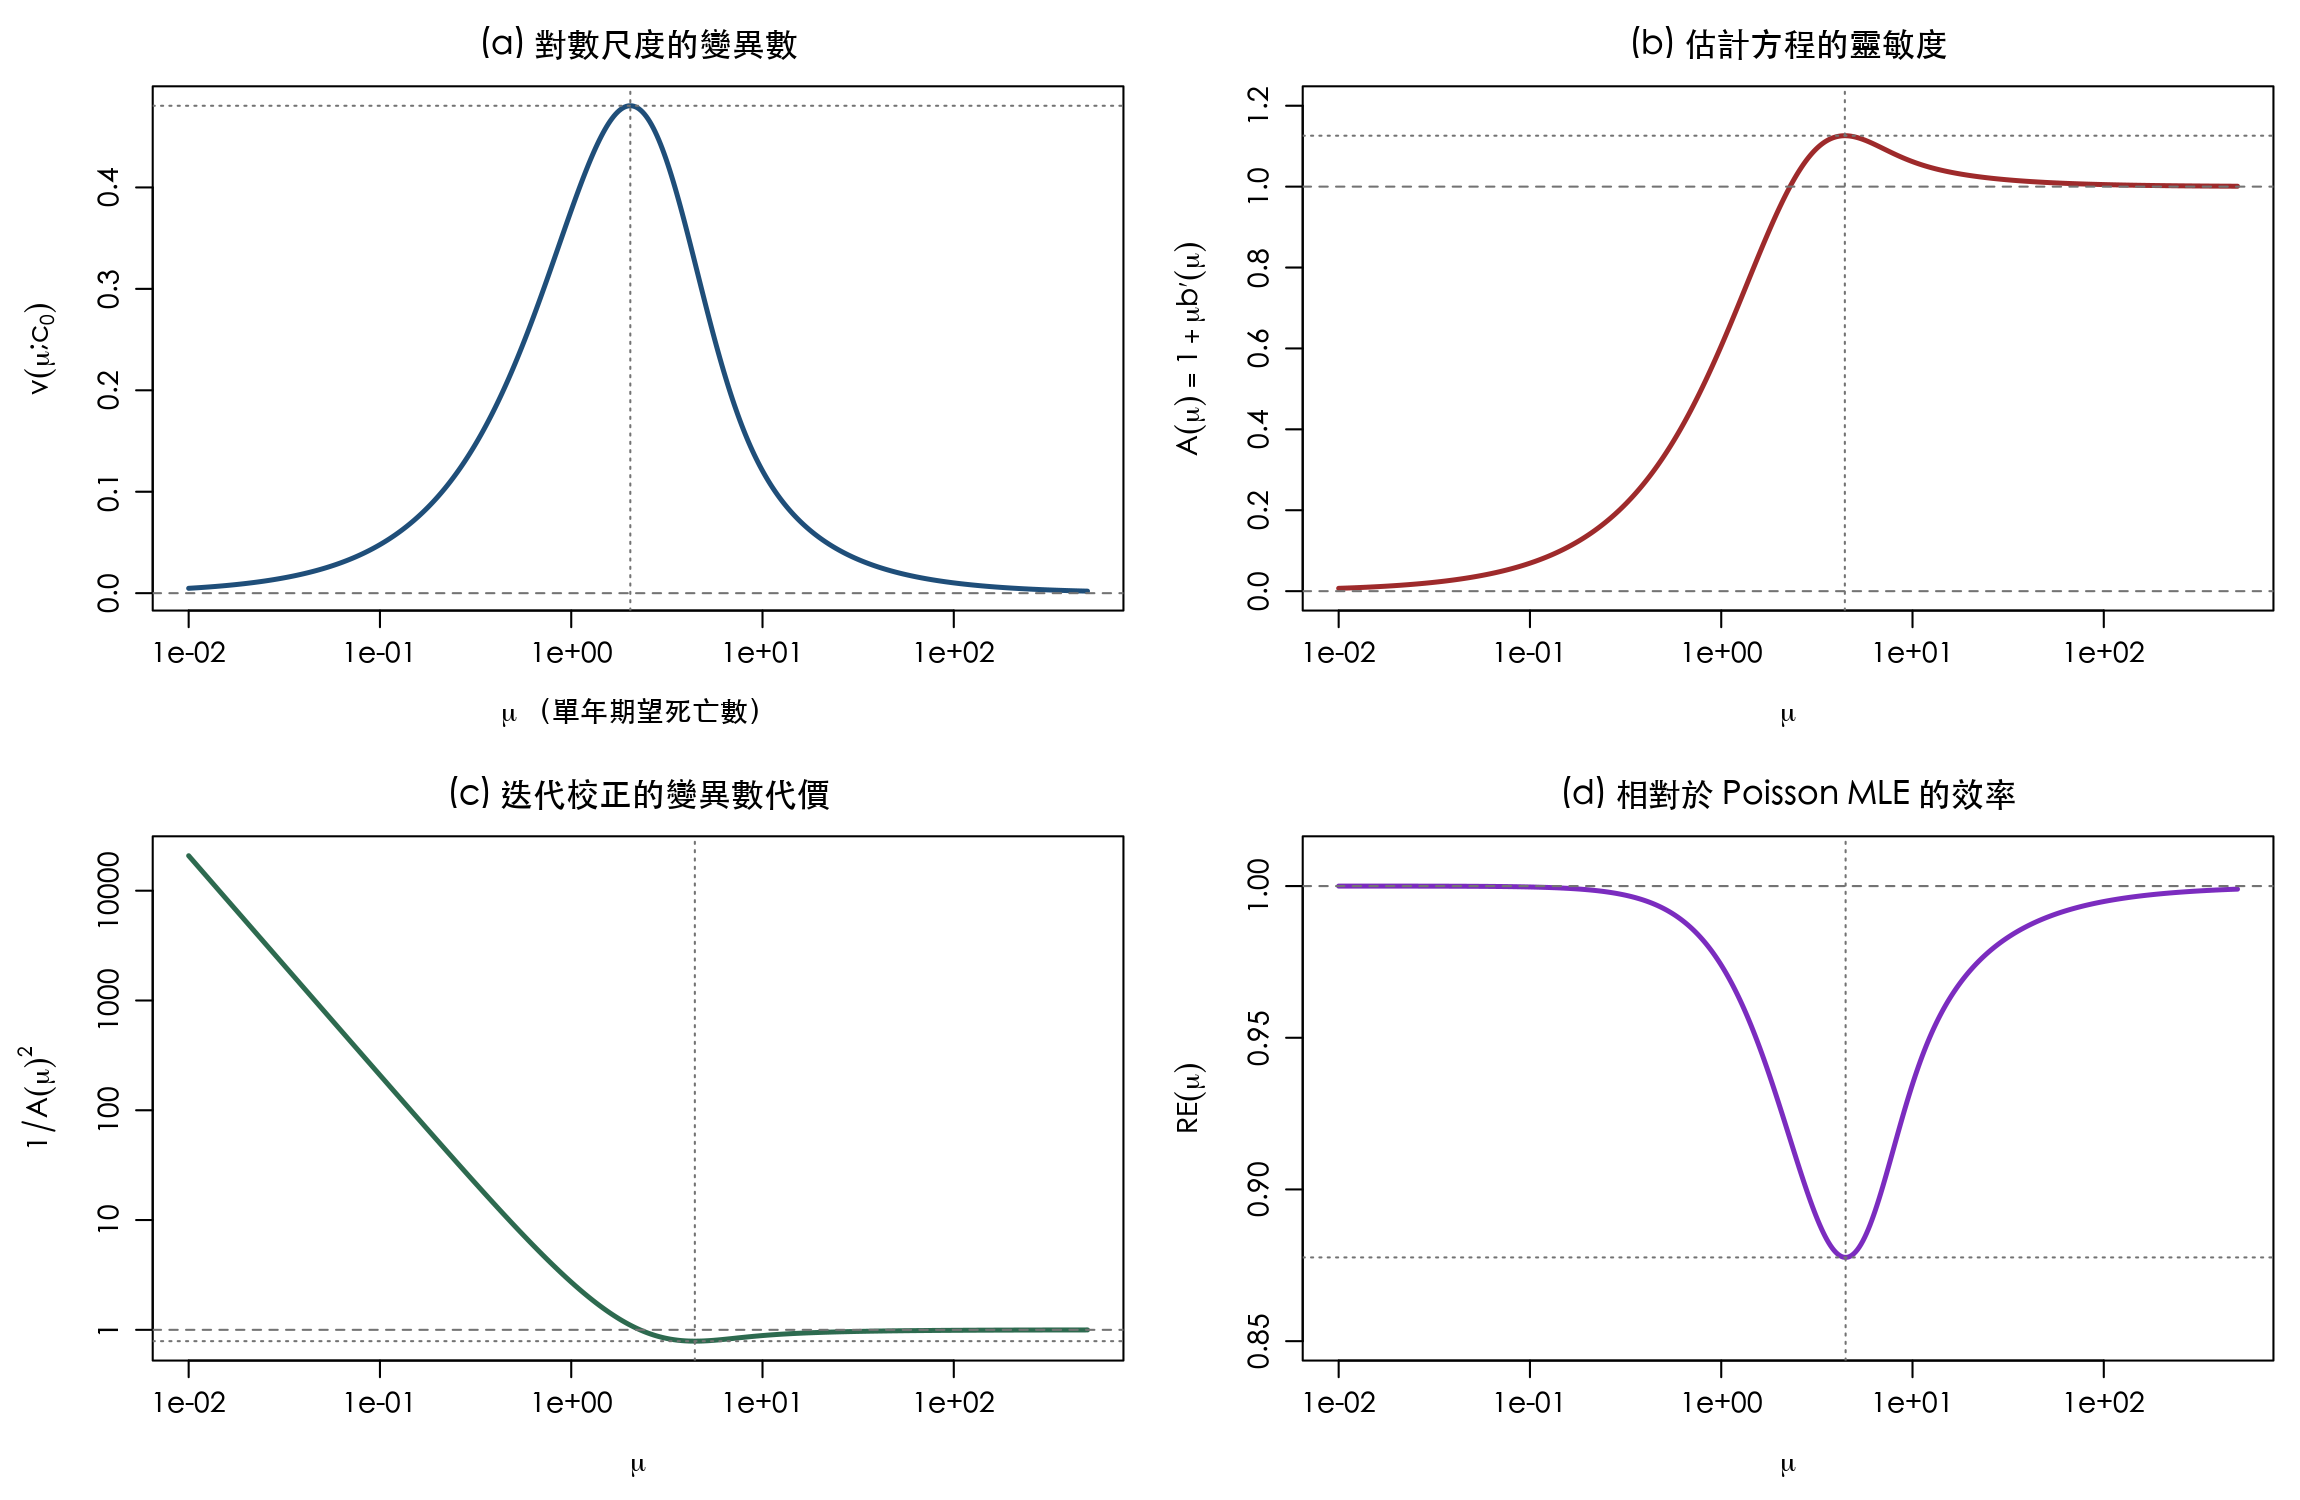
\includegraphics[width=\textwidth]{figV1_logvar.png}
\caption{四個二階解析量對期望死亡數的變化（$c_0=0.5$，橫軸取對數）}

{\footnotesize 註：(a) $v(\mu;c_0)$，於 $\mu=2.04$ 取極大 $0.481$；(b) $A(\mu)=1+\mu b'(\mu)$，於 $\mu=4.43$ 取極大 $1.126$；(c) $1/A(\mu)^2$，縱軸亦取對數，$\mu\to0$ 時發散、於 $\mu=4.43$ 取極小 $0.789$；(d) 相對於 Poisson 最大概似的效率，於 $\mu=4.47$ 取極小 $0.878$。}

\label{fig:v}
\end{figure}

四個量的最差處落在 $\mu$ 軸的不同位置。
偏誤 $b$ 在 $\mu\to0$ 最大，變異數 $v$ 在 $\mu=2.04$ 最大，
校正的代價在 $\mu\to0$ 發散而於 $\mu=4.43$ 最小，
效率則在 $\mu=4.47$ 最低。
亦即幼年組的問題是偏誤與校正的代價，中年組的問題是變異數與效率，
而高齡組兩者皆小。這張圖於是可以一眼讀出各年齡各自該擔心的項目。

(a) 與 (c) 的對照另有一項實務意涵。$v$ 在 $\mu\to0$ 時趨於零，
因此零格主導的年齡其 $\hat\alpha_x$ 的抽樣變異很小，帶窄而偏誤大；
但 $1/A^2$ 在同一處發散，因此校正把該處的帶重新放大。
兩者合起來說明：校正把偏誤換成了變異，而換算的匯率在幼年組極為不利，
這正是第\ref{sec:lim}所述「校正在最需要它的時候自動失效」的二階版本。
就本節與下一節的接續而言，五個量都只透過期望死亡數進入，
而期望死亡數由曝露數與一組粗略死亡率即可算出；
這一點正是第\ref{sec:feas}節的事前檢定得以成立的基礎。


本節與第\ref{sec:method}節的結果都是有限樣本的陳述，不依賴任何漸近敘述，
此處把這一點明白寫出，以免讀者誤以為有未交代的漸近條件。
Corollary~\ref{cor:alpha} 的 $\Ex[\hat\alpha_x]-\alpha_x=\bar b_x$ 是一個
\textbf{恆等式}：只要式~\eqref{eq:pois} 的 Poisson 假設成立、
且 $\hat\alpha_x$ 依式~\eqref{eq:svd} 定義為列平均，該式對任意的 $T$ 成立，
不需要 $T\to\infty$，也不含 $O(T^{-1})$ 的餘項。
這與古典的小樣本偏誤結果不同：\citet{coxsnell1968} 與 \citet{firth1993}
所處理的是最大概似估計量 $O(n^{-1})$ 的漸近偏誤，
其修正的正當性建立在該展開之上；而本文的偏誤項是精確的。
同理 Corollary~\ref{cor:var} 的變異數、Proposition~\ref{prop:infl} 的
靈敏度與 Corollary~\ref{cor:re} 的效率，都是逐格的精確計算，
其唯一的近似出現在 Proposition~\ref{prop:infl} 由一階展開得到的代價
$1/A^2$；該近似的有效範圍已於第\ref{sec:vinfl}以數值界定。

兩項與漸近有關的事實則可直接由前述結果讀出，不需要另立命題。
其一，$b(\mu;c_0)$ 不隨觀測年數 $T$ 增加而消失，
蓋因式~\eqref{eq:bform} 完全不含 $T$；標準 Lee-Carter 的 $\hat\alpha_x$ 在
期望死亡數有界的情形下不一致，而扣除 $\bar b_x$ 後一致。
其二，$N\to\infty$ 使 $\mu\to\infty$ 時 $b\to-1/(2\mu)\to0$，
於是在大母體的設定下標準 Lee-Carter 與所提的修正皆一致，兩者的差別為 $O(N^{-1})$。
這兩點各只是式~\eqref{eq:bform} 與式~\eqref{eq:jensen} 的直接後果。

至於把 $\hat\beta_x$ 與 $\hat\kappa_t$ 納入同一框架所需的漸近理論，
其困難不在上述兩點，而在 $\hat\kappa_t$ 的個數隨 $T$ 一同增長，
屬增長參數維度的問題；在小區域估計的文獻中，
\citet{lahiri2023} 的巢式誤差迴歸為目前最接近的工具。
$\hat\beta_x$ 一側則須以逐元的矩陣擾動理論處理（\citealp{abbe2020}），
而非以子空間的角度界限處理（\citealp{caizhang2018}），
且因各格的變異數 $v(\mu_{x,t})$ 相差可達百倍，須採異質變異的版本
（\citealp{zhang2022}）。本文不作此項推導，於第\ref{subsec:future}列為後續工作。

\section{以臺灣資料驗證}\label{sec:valid}

本節以臺灣女性的死亡資料核對前兩節的推導。
前兩節所導出的各式各自給出一項可檢驗的預測，表~\ref{tab:pred} 先把它們與
檢驗的位置並列，使讀者在進入數字之前即知道每一項的賭注為何。
其中第四項是\textbf{反向}的預測，亦即理論要求某一項指標\textbf{不}改善；
此類預測有風險，蓋因若偏誤的來源不是推導所描述的那一個，
該項指標沒有理由恰好不動，故其成立比正向預測更具證據力。

\begin{table}[H]
\centering
\caption{前兩節所給出的預測與其檢驗位置}
\footnotesize
\begin{tabular}{llll}
\toprule
預測 & 出處 & 檢驗於 & 結果\\
\midrule
$\hat\alpha_x$ 的偏誤恰為 $\bar b_x$，逐年齡皆然
  & Cor.~\ref{cor:alpha} & 第\ref{sec:closedfit} & 相關係數 $\ge0.988$\\
總人數固定下改變年齡結構，偏誤的變化全由 $b(\mu)$ 決定
  & Prop.~\ref{prop:fisher} & 第\ref{sec:popstr} & 相關係數 $\ge0.998$\\
中心化應大幅移除 $\alpha_x$ 的偏誤
  & 式~\eqref{eq:center} & 第\ref{sec:empmain} & 中位偏誤降 $2.3$--$7.2$ 倍\\
中心化\textbf{不應}改善漂移項
  & 式~\eqref{eq:center} & 第\ref{sec:empmain} & $0.3436\to0.3544$，未改善\\
校正只移動中心、不改變離散
  & 式~\eqref{eq:center} & 第\ref{sec:e0var} & 標準差 $0.613\to0.613$\\
取對數的效率損失不超過 $12.2\%$
  & Cor.~\ref{cor:re} & 第\ref{sec:vcheck} & 逐年齡最低 $0.879$\\
\bottomrule
\end{tabular}
\label{tab:pred}
\end{table}

所用的資料與模擬設定於前兩小節
一次交代，其後依序核對偏誤的閉式、人口年齡結構對偏誤的影響、
四個二階解析量的數值，以及校正所付變異數代價的有效範圍。

\subsection{研究資料與模擬設定}\label{subsec:data}\label{sec:setup}

本文所用的資料取自 Human Mortality Database 的臺灣女性 2001 至 2024 年
死亡數與曝露數，聚合為 $A=22$ 個五齡組（$0$、$1$--$4$、$5$--$9$、\dots、
$95$--$99$、$100^{+}$），年份數 $T=24$。
之所以不採單齡組，是因為單齡組在鄉鎮市區的規模下零死亡格的比例過高，
使各年齡的估計幾乎只由替代值決定，而五齡組是官方生命表與既有小區域
研究所採的分組方式，便於與其結果對照。
全部分析只用女性。女性的死亡率曲線較平滑，可使驗證不混入模型誤設；
更要緊的是本文的閉式只透過期望死亡數進入偏誤，性別本身不是閉式中的變數，
男性的差異僅反映為期望死亡數水準的不同，因此以女性為例不失一般性。
全性別合併的情形因兩性死亡率型態不同而需另設模型，本文不予處理。

真值定義為全國資料的 Poisson 最大概似配適
$(\alpha^{0}_x,\beta^{0}_x,\kappa^{0}_t)$，其隱含的死亡率為
$m^{0}_{x,t}=\exp(\alpha^{0}_x+\beta^{0}_x\kappa^{0}_t)$。
以配適值而非觀測值為真值的理由是：本文所要檢驗的是估計程序對給定期望
死亡數的反應，真值必須落在模型內；觀測值偏離模型的影響另於
第\ref{sec:real}以真實死亡數的抽薄單獨處理。
小人口的曝露數則設為 $E_{x,t}=N\,w_x$，其中 $N$ 為單一性別的總人數、
$w_x$ 為年齡結構，除第\ref{sec:popstr}另行指定者外一律取 2024 年全國
女性的曝露結構（$65$ 歲以上占 $20.3\%$）且不隨年份變動，
以使不同規模之間的比較只反映人數的差異。
人數取一萬、五萬與二十萬三個水準，涵蓋我國鄉鎮市區的主要範圍：
368 個鄉鎮市區中有 217 個的單一性別人數在兩萬以下、299 個少於五萬，
而二十萬一級則對應全國少數人口較多的市區。
模擬的重複次數、亂數種子、比較指標與計算環境如下。


第\ref{sec:valid}節與第\ref{sec:result}節的所有模擬共用同一組設定，
以下一次寫定其執行細節。

\textbf{重複與亂數。} 各組合重複 $R=100$ 次，死亡數依式~\eqref{eq:pois}
以 \texttt{rpois} 產生。亂數種子固定為
$\text{seed}=20260926+1000\,i+r$，其中 $i$ 為人口規模的序號、
$r$ 為重複的序號；第\ref{sec:valid}節、第\ref{sec:empmain}至第\ref{sec:e0var}
與第\ref{sec:joint}沿用同一組種子，因此各表可逐格對照，
不同估計量之間的差異不含蒙地卡羅的雜訊。
第\ref{sec:smr}（參考母體）與第\ref{sec:real}（真實資料抽薄）因需額外的亂數，
採 $20260926+11000\,i+97\,s+r$ 與 $20260926+7000\,i+r$ 兩組，
其中 $s$ 為情境的序號。

\textbf{比較指標。} 四項指標分別對應四個標的。
$\alpha$ 的偏誤取各年齡 $\hat\alpha_x-\alpha^{0}_x$ 在 $R$ 次重複中的中位數，
再取其絕對值的中位數與最大值，前者刻畫整體水準、後者刻畫最差的年齡。
$\beta$ 的誤差取相對平方誤差和
$\mathrm{SSE}(\beta)=\sum_x(\hat\beta_x-\beta^{0}_x)^2\big/\sum_x(\beta^{0}_x)^2$。
時間參數以漂移項 $(\hat\kappa_T-\hat\kappa_1)/(T-1)$ 與真值之差表示。
最終標的為配適末年的零歲平均餘命，依均勻死亡假設編算簡易生命表，
最高年齡組為 $100$ 歲以上，其平均餘命取 $1/m_{A}$。
離散度另以 $R$ 次重複的標準差、四分位距與全距表示。

\textbf{計算環境。} 本文所比較的各估計量皆以 R 自行實作，不依賴外部套件。%
\footnote{R 4.2.1（x86\_64-apple-darwin17.0）；除讀取 Excel 檔的
\texttt{readxl} 與稀疏矩陣的 \texttt{Matrix} 外不依賴外部套件。
奇異值分解採內建的 \texttt{svd}（LAPACK），Poisson 配適採自行撰寫的疊代重
加權最小平方，收斂門檻為參數變動的最大絕對值小於 $10^{-10}$。
程式置於 \texttt{R/core/} 與 \texttt{R/studies/}，
各節所引的表格編號與產生該表的程式檔名一一對應。}


\subsection{驗證的設計與閉式預測的對照}\label{subsec:vdesign}\label{sec:closedfit}

Corollary~\ref{cor:alpha} 是恆等式，驗證的對象於是不是數學本身，
而是\textbf{推導所描述的那個量與實際估計流程所產生的那個量是否為同一個}：
後者含奇異值分解、識別條件的正規化，以及 $\hat\beta_x\hat\kappa_t$ 的估計
誤差向 $\hat\alpha_x$ 的滲透。

資料、真值、人口規模與亂數種子均依第\ref{sec:setup}所定。
此一設計有兩項代價須先承認。一方面，它假設小人口的
死亡率\textbf{恰好}等於全國的死亡率，而真實的鄉鎮市區顯然不是如此；
但本節的目的是檢驗閉式，而閉式所刻畫的是估計程序對給定 $\mu_{x,t}$ 的
反應，與該 $\mu_{x,t}$ 是否貼近某個真實地區無關。另一方面，它使資料恰好落在
秩一雙線性結構上，因此排除了模型誤設；這一點在本節是優點，
若連如此單純的情形都無法吻合，推導即有問題；但也使本節的結論須由
第\ref{sec:real}補上另一半。

每一次重複皆以標準 Lee-Carter 估計，取各年齡 $\hat\alpha_x-\alpha^{0}_x$ 在 100 次
重複中的中位數作為該年齡的實測偏誤，再與 Corollary~\ref{cor:alpha} 的
預測值 $\bar b_x=T^{-1}\sum_t b(\mu_{x,t};c_0)$ 比較。
比較的方式有二：逐年齡的相關係數，以及以預測值為自變數、實測值為應變數的
迴歸斜率；前者檢驗\textbf{形狀}是否一致，後者檢驗\textbf{量級}是否一致。
兩者都接近 $1$ 才算通過。


\begin{table}[H]
\centering
\caption{閉式預測與模擬實測的對照（標準 Lee-Carter，重複 100 次）}
\small
\begin{tabular}{lrrr}
\toprule
 & $N=10^4$ & $N=5\times10^4$ & $N=2\times10^5$\\
\midrule
逐年齡的相關係數 & \textbf{1.000} & \textbf{1.000} & \textbf{0.988}\\
迴歸斜率（實測對預測） & 1.001 & 0.990 & 0.962\\
殘差量級 & $\sim$0.01 & $\sim$0.01 & $\sim$0.02\\
\bottomrule
\end{tabular}
\label{tab:valid}
\end{table}

表~\ref{tab:valid} 顯示形狀與量級都通過。逐年齡的相關係數在三個規模下
分別為 $1.000$、$1.000$、$0.988$，迴歸斜率為 $1.001$、$0.990$、$0.962$，
兩者都接近 $1$；殘差的量級約為 $0.01$ 至 $0.02$，而重複 100 次時
$\alpha$ 偏誤的蒙地卡羅誤差本就約有一成，以人數五萬時 5 至 9 歲組的
$0.87$ 計即約 $0.09$，因此 $0.01$ 的殘差已在雜訊之內。
人數二十萬時相關係數與斜率略低（$0.988$ 與 $0.962$），
原因是該規模下各年齡的絕對偏誤已降到 $0.1$ 以下，
蒙地卡羅誤差相對於待測的量變大，並非推導本身在該處失準。

表~\ref{tab:validage} 進一步列出逐年齡的對照；這張表同時展示了
第\ref{sec:normal}前所導出的兩個門檻。先看中位數的崩潰門檻
$\mu<\ln2=0.693$：1 至 4 歲、5 至 9 歲、10 至 14 歲三組的單年期望死亡數
皆為 $0.3$，其零格比例 $\pi=e^{-0.3}=0.74$ 已遠超過 $50\%$，
15 至 19 歲組的 $0.5$ 人對應 $\pi=0.61$ 亦然；
這四組於是落在穩健損失的作用範圍之外，而它們恰好也是偏誤最大的四組
（$0.33$ 至 $0.87$）。再看偏誤的變號門檻 $\mu^\ast=0.9234$：
20 至 24 歲組的期望死亡數為 $0.9$，恰在門檻上，其偏誤因此僅 $+0.04$，
幾乎為零；而零歲組的 $1.2$ 人已越過門檻，偏誤轉為 $-0.07$。
兩個門檻所預測的位置與實測一一對應，且都可由死亡數直接算出，
不需要真值，這正是把閉式寫出來的實用價值所在。

\begin{table}[H]
\centering
\caption{逐年齡對照（人數五萬，選列）}
\small
\begin{tabular}{lrrrrr}
\toprule
年齡組 & 單年期望死亡數 & $\pi=e^{-\mu}$ & 閉式預測 & 模擬實測 & 差\\
\midrule
0      & 1.2  & 0.30 & $-0.0753$ & $-0.0692$ & $+0.0061$\\
1--4   & 0.3  & \textbf{0.74} & $0.7283$  & $0.7135$  & $-0.0148$\\
5--9   & 0.3  & \textbf{0.77} & $0.8689$  & $0.8658$  & $-0.0031$\\
10--14 & 0.3  & \textbf{0.77} & $0.8341$  & $0.8262$  & $-0.0079$\\
15--19 & 0.5  & \textbf{0.61} & $0.3298$  & $0.3386$  & $+0.0088$\\
20--24 & 0.9  & 0.41 & $0.0415$  & $0.0529$  & $+0.0114$\\
45--49 & 7.3  & 0.00 & $-0.0793$ & $-0.0831$ & $-0.0038$\\
70--74 & 48.8 & 0.00 & $-0.0108$ & $-0.0135$ & $-0.0027$\\
85--89 & 73.9 & 0.00 & $-0.0069$ & $-0.0061$ & $+0.0008$\\
\bottomrule
\end{tabular}
\label{tab:validage}
\end{table}

圖~\ref{fig:aband} 以圖的形式呈現同一組結果，其設計是在兩個人口規模下，
把標準 Lee-Carter 與中心化兩個估計量的逐年齡偏誤分布與閉式預測畫在同一張圖上。
圖中紅色區域為標準 Lee-Carter 在 100 次重複中 $\hat\alpha_x-\alpha_x$ 的
$5$ 至 $95$ 百分位帶，紅線為其中線，藍色為中心化的對應結果，
黑色虛線則是 Corollary~\ref{cor:alpha} 的閉式預測 $\bar b_x$。
之所以用帶而不用單一數字，是因為偏誤與變異在圖上有截然不同的樣子，
而表只能呈現其中一面。

\begin{figure}[H]
\centering
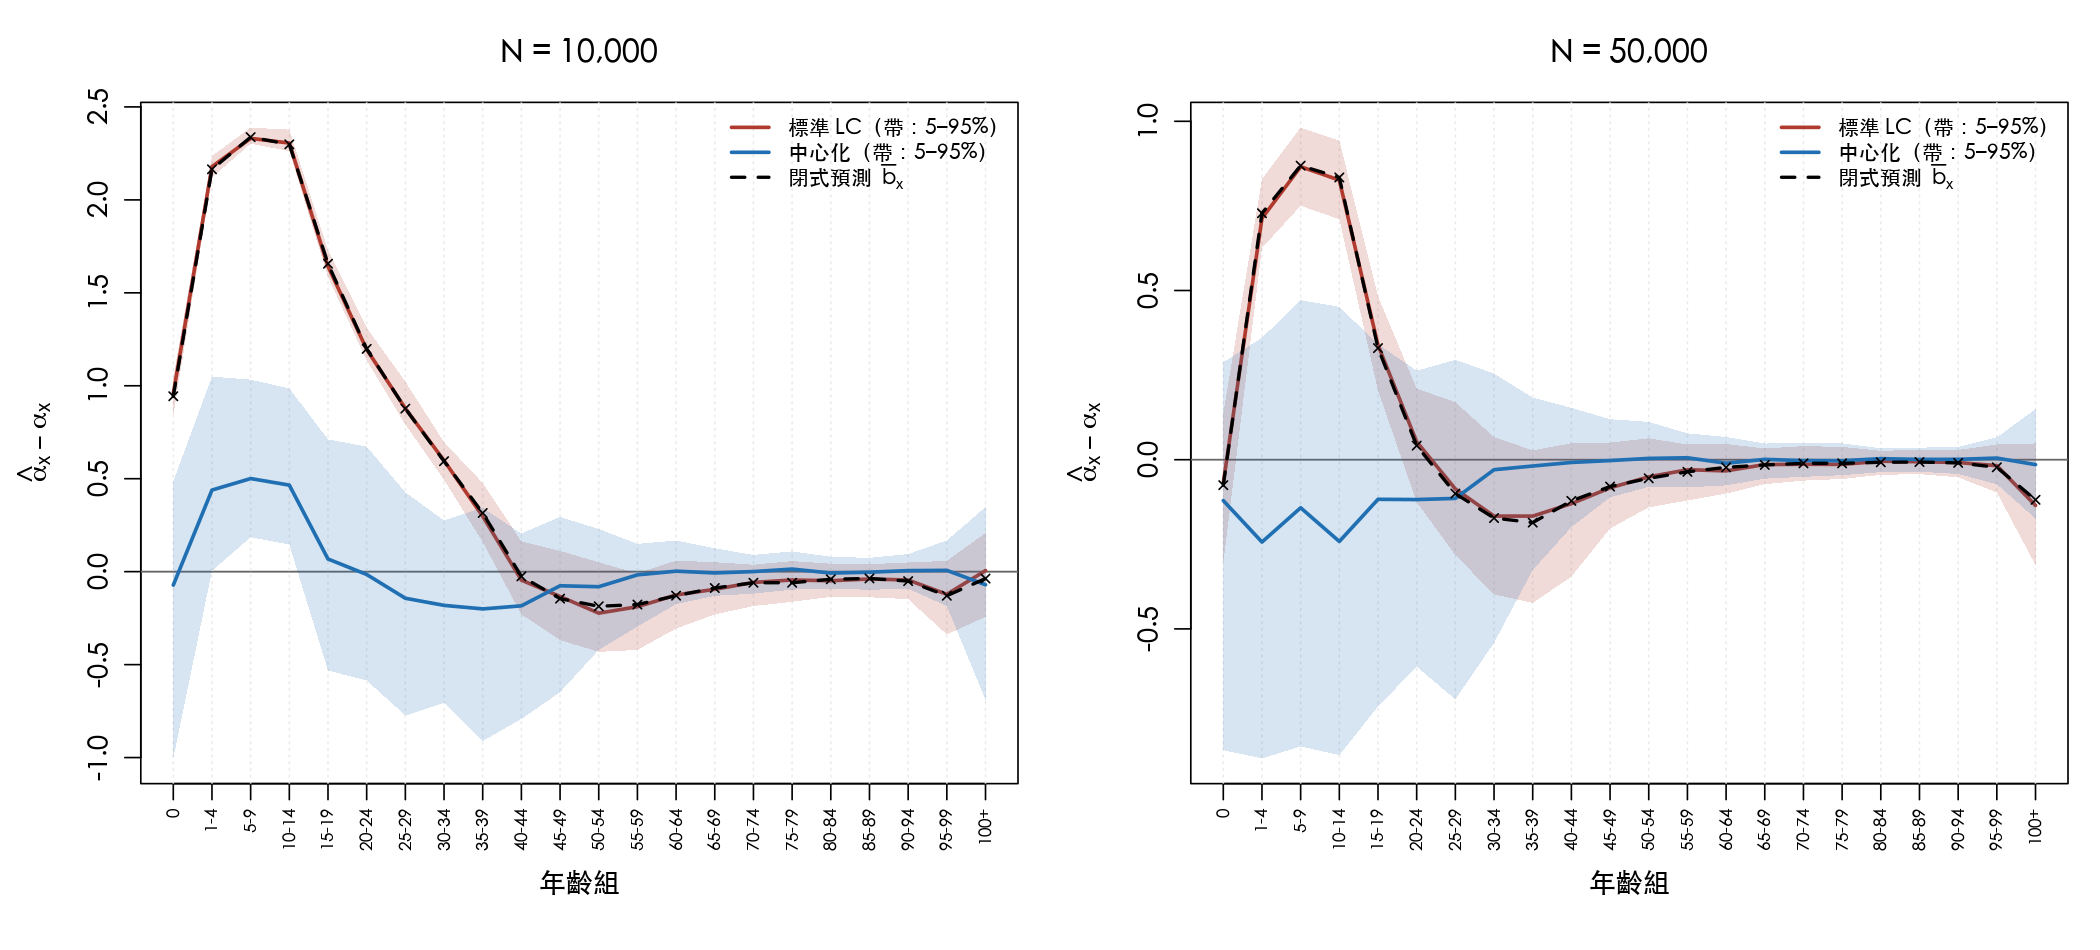
\includegraphics[width=\textwidth]{figT1_alpha_band.png}
\caption{$\hat\alpha_x$ 的偏誤：5--95\% 帶與閉式預測}

{\footnotesize 註：黑色虛線為 Corollary~\ref{cor:alpha} 的預測值 $\bar b_x$，與標準 Lee-Carter 的中線最大差 $0.043$ 與 $0.019$。}

\label{fig:aband}
\end{figure}

由圖中可以看到，黑色虛線幾乎完全落在紅線上，兩者的最大差在兩個規模下
分別為 $0.043$ 與 $0.019$，而偏誤本身在 5 至 9 歲組達 $2.33$ 與 $0.87$。
這與 Corollary~\ref{cor:alpha} 的內容吻合，該式所主張的正是
$\hat\alpha_x$ 的期望等於真值加上 $\bar b_x$。
與此相對，標準 Lee-Carter 的帶明顯偏窄，人數五萬時帶寬中位為 $0.218$，
而 5 至 9 歲組的偏誤為 $0.866$，偏誤是帶寬的四倍；
亦即該年齡幾乎每一次模擬都落在真值的同一側。
這對應第\ref{subsec:mest}所述的分工：帶寬反映的是估計方程的變異數，
中線的位置反映的是其期望，而 Fisher 不一致動的是後者。
這也說明了既有文獻以重複抽樣觀察小人口 Lee-Carter 時，
所見為震盪而非偏誤的原因。

中心化之後的情形則不同。中心化雖把中線拉回零附近，
帶卻由 $0.218$ 變寬為 $0.277$（人數五萬），且在幼年組變寬得更多。
這一點不是閉式本身的問題，而是來自閉式必須代入估計值 $\hat\mu_{x,t}$：
$b$ 是確定性的函數，但 $b(\hat\mu)$ 不是，代入的動作把 $\hat\mu$ 的噪音
帶進每一格。由於幼年組的 $\hat\mu$ 本身最不精確，變寬也集中在該處。
這構成所提修正的一項代價，第\ref{sec:joint}將說明如何以
「只扣列平均、不逐格扣除」的設計把這項代價移除。
這張圖說明的是標準 Lee-Carter 的 $\alpha_x$ 誤差以偏誤為主而非以變異為主，
且該偏誤的大小可由閉式事先算出；而中心化能把偏誤移除，代價是變異略增。

綜合表~\ref{tab:valid}、表~\ref{tab:validage} 與圖~\ref{fig:aband}，
本節的結論是推導所描述的量確實就是實際估計流程所產生的量：
奇異值分解與識別條件的正規化並未把 $\hat\alpha_x$ 帶動，
$\hat\beta$ 與 $\hat\kappa$ 的估計誤差也未明顯滲入。
這把先前只能以模擬描述的現象變成一個可計算的量，標準 Lee-Carter 的 $\alpha_x$
偏誤\textbf{完全}由各格期望死亡數的一個確定性函數決定，不含未知成分。
既然如此，該量即可計算並扣除，此即下一節的工作。
須補充的是，本節情境的單純性係由設計而來：資料恰好落在秩一結構上、
分布恰好是 Poisson 。真實資料兩者都不完全成立，
因此第\ref{sec:real}將以實際觀測的死亡數重做一次，檢驗結論是否仍然成立。

\subsection{人口年齡結構的影響}\label{sec:popstr}

前一小節的驗證在單一的年齡結構下進行。但閉式 $b(\mu;c_0)$ 只透過期望死亡數
$\mu_{x,t}=E_{x,t}m_{x,t}=N w_x m_{x,t}$ 進入偏誤，而 $w_x$ 正是年齡結構；
於是閉式對本問題給出一個更嚴格的可檢驗預測：
\textbf{在總人數 $N$ 固定下改變 $w_x$，標準 Lee-Carter 的逐年齡偏誤應隨之改變，
且改變的方向與幅度完全由 $b(\mu)$ 決定}。
這比「偏誤隨 $N$ 而變」更嚴格，因為此處資訊總量不變，
變的只是資訊在年齡之間的分配。本小節檢驗此一預測，
並一併給出鄉鎮市區應用上的一項實務依據，即在同為五萬人的地區之間，
人口老化程度對 Lee-Carter 估計可信度的影響。

三組結構皆以臺灣女性的實際曝露數為本。年輕結構取 2001 年的全國結構
（$65$ 歲以上占 $8.5\%$），基準結構取 2024 年（$20.3\%$），
高齡結構則以 2024 年結構作指數傾斜 $w_x\propto w_x^{2024}e^{0.085(x-1)}$，
使 $65$ 歲以上占 $31.7\%$，對應人口外流的鄉鎮市區。
三者的總人數相同，真實死亡率 $m^{0}_{x,t}$ 亦相同，差別只在年齡分配。

\begin{table}[H]
\centering
\caption{人口年齡結構對偏誤的影響（人口總數固定於五萬，重複 100 次）}
\small
\renewcommand{\arraystretch}{1.15}
\begin{tabular}{llrrrrr}
\toprule
結構 & 估計量 & $\alpha$ 中位 & $\alpha$ 最大 & SSE($\beta$) & $e_0$ 偏誤 & $e_0$ 標準差\\
\midrule
\multirow{3}{*}{年輕（$65^{+}$ 占 $8.5\%$）}
 & 標準 Lee-Carter      & 0.0907 & 0.4275 & 4.2032 & $-1.055$ & 0.897\\
 & Firth        & 0.0111 & \textbf{0.0416} & 1.3418 & $-0.318$ & 0.838\\
 & 中心化＋加權 & 0.0393 & 0.0865 & \textbf{1.0960} & \textbf{$-0.235$} & 0.973\\
\addlinespace
\multirow{3}{*}{基準（$20.3\%$）}
 & 標準 Lee-Carter      & 0.0596 & 0.8658 & 3.9369 & $-1.415$ & 0.626\\
 & Firth        & 0.0057 & \textbf{0.0724} & 1.6656 & $-0.182$ & 0.429\\
 & 中心化＋加權 & 0.0213 & 0.0735 & \textbf{1.1366} & \textbf{$+0.057$} & 0.564\\
\addlinespace
\multirow{3}{*}{高齡（$31.7\%$）}
 & 標準 Lee-Carter      & 0.0492 & 1.4555 & 6.2652 & $-2.109$ & 0.685\\
 & Firth        & 0.0070 & \textbf{0.1276} & 2.9394 & $-0.210$ & 0.418\\
 & 中心化＋加權 & 0.0187 & 0.1110 & \textbf{1.2424} & \textbf{$+0.066$} & 0.517\\
\bottomrule
\end{tabular}

{\footnotesize 註：三種結構的真實死亡率相同。}

\label{tab:popstr}
\end{table}

標準 Lee-Carter 一列隨結構老化而系統性地惡化：
$\alpha$ 最大偏誤由年輕結構的 $0.428$ 上升到高齡結構的 $1.456$，
約為三點四倍；零歲平均餘命的偏誤由 $-1.055$ 歲擴大到 $-2.109$ 歲，正好一倍。
作為對照，在基準結構下把人數由五萬降到一萬才使 $e_0$ 偏誤由 $-1.415$
擴大到 $-3.725$ 歲，可見人口老化對估計品質的傷害與人口減少屬同一量級。
這與第\ref{subsec:bprops}所推導的 $b(\mu;c_0)$ 形狀吻合。
蓋因高齡結構把曝露數由幼年組移往高齡組，使幼年組的 $\mu_{x,t}$ 更小、
$b(\mu)=\log(c_0/\mu)$ 更大；而高齡組的 $\mu$ 雖然增加，
$b$ 在該端卻只以 $-1/(2\mu)$ 的速率趨近零，兩端並不對稱，
因此曝露數的重新分配並不會相互抵銷，整體偏誤因此惡化。

閉式的準確度在三種結構下都成立。以 $\bar b_x$ 預測逐年齡實測偏誤，
三種結構的相關係數分別為 $0.998$、$0.999$、$1.000$，
迴歸斜率為 $0.959$、$0.987$、$0.986$；人數一萬時相關係數皆為 $1.000$、
斜率為 $0.995$、$0.996$、$1.001$。
由於三組結構下的 $\mu_{x,t}$ 完全不同，而同一個函數在三組之上都準確，
此一結果比第\ref{sec:closedfit}的單一結構驗證更強，
顯示閉式所捕捉的並非某一組曝露數的巧合，而是估計程序對 $\mu$ 的反應。
就應用而言，這意味分析者只要有曝露數與一組初步的死亡率估計，
即可在不做任何模擬的情形下事先算出該地區的 Lee-Carter 估計會偏多少。

至於校正之後的結果，三種結構之間的差異已大致消失：
中心化加權的 $e_0$ 偏誤分別為 $-0.235$、$+0.057$、$+0.066$ 歲，全距 $0.30$ 歲；
而未校正者為 $-1.055$、$-1.415$、$-2.109$ 歲，全距 $1.05$ 歲，
$\alpha$ 最大偏誤的全距亦由 $1.03$ 降至 $0.025$。
這是扣除 $b(\mu_{x,t})$ 的必然結果，蓋因結構正是透過 $\mu$ 進入偏誤的，
扣掉 $b$ 也就同時扣掉了結構的影響。

表中不利於本文的部分同樣須說明。Firth 在 $\alpha$ 最大偏誤上仍然略勝
（$0.042$、$0.072$、$0.128$ 對 $0.087$、$0.074$、$0.111$），
與第\ref{sec:empmain}的結果一致，原因在於事後扣除只能移除期望值的偏移，
而 Firth 從源頭不產生該筆錯誤資訊。另外，人數一萬時的結論須保留：
該規模下中心化加權的 $e_0$ 偏誤為 $-2.542$、$-1.200$、$-0.636$ 歲，
雖較標準 Lee-Carter 的 $-1.858$、$-3.725$、$-6.987$ 有大幅改善，
但年輕結構下反而劣於標準 Lee-Carter。
這並非閉式失準，而是閉式必須代入 $\hat\mu$ 所致：
年輕結構把曝露數集中在死亡率極低的年齡，使該處的 $\hat\mu$ 本身幾無資訊，
代入後所扣的量遠小於應扣的量，校正於是在最需要它的地方自動失效。
此一現象構成本文方法的規模下界，第\ref{sec:disc}節列為限制。

總體而言，這張表所呈現的是：小人口 Lee-Carter 的偏誤不只是「人少」的問題，
也是「人口結構」的問題；兩者都可由同一個閉式解釋；
校正不僅縮小偏誤，也移除了偏誤對年齡結構的依賴，
但其有效範圍受限於 $\hat\mu$ 本身是否仍有資訊。


\subsection{二階解析量的數值核對}\label{sec:vcheck}\label{sec:vsd}\label{sec:vinfl}

前三小節的驗證針對一階的閉式，本小節則針對第\ref{sec:second2}節的四個
二階解析量。其中 Proposition~\ref{prop:v}、Proposition~\ref{prop:bp} 與
Corollary~\ref{cor:re} 為恆等式，嚴格說來不需要檢驗，
但三式都含無窮級數，截斷的位置可能影響結果，因此先以模擬核對其實作；
Proposition~\ref{prop:infl} 的代價含一階展開，其有效範圍則於本小節末以
數值界定。

\begin{table}[H]
\centering
\caption{四個二階解析量的值與數值核對（$c_0=0.5$）}
\small
\begin{tabular}{rrrrrrrr}
\toprule
$\mu$ & $b(\mu)$ & $v(\mu)$ & 模擬 $v$ & $\mu b'(\mu)$ & $A(\mu)$ & $1/A^2$ & $\mathrm{RE}$\\
\midrule
0.02   & $3.2327$  & 0.0096 & 0.0095 & $-0.9861$ & 0.014 & 5204.3 & 1.0000\\
0.05   & $2.3372$  & 0.0240 & 0.0241 & $-0.9654$ & 0.035 & 833.4  & 0.9999\\
0.10   & $1.6787$  & 0.0479 & 0.0479 & $-0.9308$ & 0.069 & 209.0  & 0.9997\\
0.30   & $0.7176$  & 0.1400 & 0.1401 & $-0.7954$ & 0.205 & 23.88  & 0.9973\\
0.50   & $0.3416$  & 0.2230 & 0.2230 & $-0.6673$ & 0.333 & 9.03   & 0.9926\\
0.6931 & $0.1416$  & 0.2921 & 0.2925 & $-0.5532$ & 0.447 & 5.01   & 0.9863\\
0.9234 & $0.0000$  & 0.3589 & 0.3585 & $-0.4309$ & 0.569 & 3.09   & 0.9772\\
1.00   & $-0.0329$ & 0.3774 & 0.3772 & $-0.3937$ & 0.606 & 2.72   & 0.9739\\
2.00   & $-0.1874$ & \textbf{0.4805} & 0.4807 & $-0.0555$ & 0.945 & 1.12 & 0.9283\\
5.00   & $-0.1199$ & 0.2868 & 0.2866 & $0.1228$ & 1.123 & \textbf{0.793} & \textbf{0.879}\\
10.0   & $-0.0552$ & 0.1206 & 0.1205 & $0.0618$ & 1.062 & 0.887 & 0.9347\\
20.0   & $-0.0262$ & 0.0543 & 0.0543 & $0.0274$ & 1.027 & 0.947 & 0.9721\\
50.0   & $-0.0102$ & 0.0206 & 0.0207 & $0.0104$ & 1.010 & 0.980 & 0.9896\\
100    & $-0.0050$ & 0.0102 & 0.0102 & $0.0051$ & 1.005 & 0.990 & 0.9949\\
300    & $-0.0017$ & 0.0034 & 0.0033 & $0.0017$ & 1.002 & 0.997 & 0.9983\\
\bottomrule
\end{tabular}

{\footnotesize 註：$v$ 以 $2\times10^{6}$ 次 Poisson 抽樣的樣本變異數為對照；$b'$ 與步長 $10^{-5}\mu$ 的中央差分比值在全部 15 個 $\mu$ 上皆為 $1.0000$，因此不另列。}


\vspace{3pt}
{\footnotesize $\mu=0.6931$ 為中位數失效門檻 $\ln2$，$\mu=0.9234$ 為偏誤變號點
$\mu^{\ast}$。粗體為各欄的極值。}
\label{tab:v1}
\end{table}

$v$ 的比值在 15 個 $\mu$ 上落在 $0.998$ 至 $1.006$，
而 $b'$ 與中央差分的比值一律為 $1.0000$，兩者都在蒙地卡羅誤差與浮點誤差的
量級之內。兩端的展開亦吻合：$\mu=0.02$ 時 $v=0.0096$ 而
$\mu(\log c_0)^2=0.0096$，$\mu=300$ 時 $v=0.0034$ 而 $1/\mu=0.0033$；
$\mu=0.02$ 時 $\mu b'=-0.9861$ 而 $-1-\mu\log c_0=-0.9861$，
$\mu=300$ 時 $\mu b'=0.001676$ 而 $\frac{1}{2\mu}+\frac{5}{6\mu^2}=0.001676$，
後者吻合至小數第六位。

表~\ref{tab:v1} 顯示四欄極值的位置互不重疊。
$b$ 在最左端最大，$v$ 在 $\mu=2$ 附近最大，
$1/A^2$ 在最左端發散而在 $\mu=5$ 附近最小，
$\mathrm{RE}$ 則同樣在 $\mu=5$ 附近最低而兩端趨近 $1$。
$\mathrm{RE}$ 一欄另確認了 Corollary~\ref{cor:re} 的上界：
$15$ 個 $\mu$ 中最低者為 $0.879$，與解析極小 $0.8776$ 相符。


表~\ref{tab:v2} 以人數五萬為例，列出 Corollary~\ref{cor:var} 對抽樣
標準差的預測、Corollary~\ref{cor:re} 的逐年齡效率，
以及 Proposition~\ref{prop:infl} 的代價與其實測值。
實測的校正估計量取第\ref{subsec:procedure}所定義的迭代版本，
亦即與第\ref{sec:result}節各表所用者相同。

\begin{table}[H]
\centering
\caption{逐年齡的二階量：預測與實測（人數五萬，重複 100 次）}
\small
\begin{tabular}{lrrrrrrr}
\toprule
年齡組 & $\mu$ 中位 & 閉式 sd & 實測 sd & 比值 & $A$ & $\mathrm{RE}$
 & 代價（閉式／實測）\\
\midrule
0        & 1.111  & 0.1299 & 0.1407 & 1.083 & 0.671 & 0.967 & 2.22\ \ /\ \ 2.61\\
1--4     & 0.283  & 0.0778 & 0.0740 & 0.951 & 0.214 & 0.997 & 21.9\ /\ 23.3\\
5--9     & 0.241  & 0.0707 & 0.0752 & 1.064 & 0.175 & 0.998 & 32.7\ /\ 31.5\\
10--14   & 0.254  & 0.0716 & 0.0713 & 0.996 & 0.180 & 0.998 & 31.0\ /\ 26.7\\
15--19   & 0.497  & 0.0978 & 0.0893 & 0.914 & 0.344 & 0.992 & 8.45\ /\ 8.48\\
20--24   & 0.829  & 0.1189 & 0.1019 & 0.857 & 0.533 & 0.980 & 3.52\ /\ 3.77\\
25--29   & 1.204  & 0.1324 & 0.1518 & 1.146 & 0.710 & 0.963 & 1.98\ /\ 2.05\\
30--34   & 1.720  & 0.1400 & 0.1527 & 1.091 & 0.884 & 0.938 & 1.28\ /\ 1.54\\
35--39   & 2.554  & 0.1383 & 0.1361 & 0.984 & 1.042 & 0.906 & 0.92\ /\ 1.18\\
40--44   & 4.847  & 0.1102 & 0.1097 & 0.995 & 1.122 & \textbf{0.880} & 0.79\ /\ 0.84\\
45--49   & 7.194  & 0.0868 & 0.0856 & 0.986 & 1.090 & 0.905 & 0.84\ /\ 0.83\\
50--54   & 9.921  & 0.0708 & 0.0628 & 0.888 & 1.062 & 0.935 & 0.89\ /\ 0.89\\
55--59   & 14.641 & 0.0562 & 0.0513 & 0.914 & 1.039 & 0.960 & 0.93\ /\ 0.93\\
60--64   & 22.595 & 0.0442 & 0.0454 & 1.028 & 1.024 & 0.976 & 0.95\ /\ 0.95\\
65--69   & 32.653 & 0.0363 & 0.0324 & 0.893 & 1.016 & 0.984 & 0.97\ /\ 0.97\\
70--74   & 46.185 & 0.0303 & 0.0311 & 1.026 & 1.011 & 0.989 & 0.98\ /\ 0.98\\
75--79   & 46.091 & 0.0303 & 0.0289 & 0.952 & 1.011 & 0.989 & 0.98\ /\ 0.98\\
80--84   & 64.868 & 0.0255 & 0.0231 & 0.906 & 1.008 & 0.992 & 0.98\ /\ 0.98\\
85--89   & 72.332 & 0.0241 & 0.0247 & 1.023 & 1.007 & 0.993 & 0.99\ /\ 0.99\\
90--94   & 53.280 & 0.0282 & 0.0267 & 0.947 & 1.010 & 0.990 & 0.98\ /\ 0.98\\
95--99   & 22.967 & 0.0440 & 0.0452 & 1.027 & 1.023 & 0.976 & 0.95\ /\ 0.95\\
$100^{+}$& 5.035  & 0.1086 & 0.1097 & 1.010 & 1.122 & \textbf{0.880} & 0.79\ /\ 0.81\\
\midrule
中位數    &        & 0.0712 & 0.0727 & 0.991 &       & 0.978 & 0.98\ /\ 0.98\\
\bottomrule
\end{tabular}
\label{tab:v2}
\end{table}

標準差的比值在 22 個年齡上落在 $0.857$ 至 $1.146$，中位數為 $0.991$，
其離散與 100 次重複所能給出的精度相當；
亦即\textbf{標準 Lee-Carter 的 $\alpha$ 變異數亦可由單一個期望死亡數的函數預測}，
與第\ref{sec:closedfit}對偏誤所得的結論同型。
$\mu$ 由 $0.24$ 升至 $72$ 時，閉式 sd 由 $0.0707$ 先升至 $0.1400$
（$\mu=1.72$）再降至 $0.0241$，實測完全跟上這個非單調的型態，
而該型態正是 Proposition~\ref{prop:v} 所預言者。

代價一欄的吻合涵蓋了兩個數量級：5 至 9 歲組預測 $32.7$ 而實測 $31.5$，
15 至 19 歲組 $8.45$ 對 $8.48$，25 至 29 歲組 $1.98$ 對 $2.05$，
而 $\mu>7$ 的十個年齡全部吻合至小數第二位。
其\textbf{量級}尤須寫明：迭代校正使 5 至 9 歲組的 $\alpha$ 變異數
放大三十倍以上。該處的 $v$ 本身很小（閉式 sd 僅 $0.0707$），
於是放大後的標準差為 $0.40$ 左右，尚不致使該年齡的估計失去意義；
但這一項說明了校正並非沒有代價；其代價集中在幼年組。

效率一欄則顯示相反的型態：$\mathrm{RE}$ 在幼年組接近 $1$
（1 至 4 歲組 $0.997$、5 至 9 歲組 $0.998$），
在 40 至 44 歲與 $100$ 歲以上兩組最低（$0.880$）。
逐格平均在三個規模下為 $0.958$、$0.963$、$0.964$，最低一律為 $0.878$。
換言之，\textbf{取對數在資料最稀的年齡幾乎不損失效率，
損失集中在每年死亡數個位數的年齡}，而全程的損失不超過 $12.2\%$。


表~\ref{tab:v3} 把三個人口規模的 22 個年齡依期望死亡數分段彙總，
比較校正代價的預測與實測。

\begin{table}[H]
\centering
\caption{校正代價的預測與實測，依期望死亡數分段（重複 100 次，取中位數）}
\small
\begin{tabular}{lrrrrr}
\toprule
$\mu$ 區間 & 年齡數 & sd 比值 & $\mathrm{RE}$ & 代價（閉式／實測） & 閉式$\div$實測\\
\midrule
\multicolumn{6}{l}{\textit{$N=10^{4}$}}\\
$\mu<0.2$     & 5 & 0.993 & 1.000 & 523.6\ /\ 85.0 & \textbf{6.16}\\
$0.2\le\mu<0.5$ & 3 & 1.066 & 0.998 & 34.2\ /\ 26.6 & 1.09\\
$0.5\le\mu<1$ & 2 & 0.970 & 0.983 & 5.52\ /\ 5.86 & 0.94\\
$1\le\mu<2$   & 3 & 1.106 & 0.953 & 1.59\ /\ 1.84 & 0.90\\
$2\le\mu<10$  & 6 & 1.001 & 0.898 & 0.85\ /\ 0.86 & 0.98\\
$\mu\ge10$    & 3 & 0.988 & 0.954 & 0.92\ /\ 0.91 & 1.00\\
\midrule
\multicolumn{6}{l}{\textit{$N=5\times10^{4}$}}\\
$0.2\le\mu<0.5$ & 4 & 0.973 & 0.997 & 26.4\ /\ 25.0 & 1.02\\
$0.5\le\mu<1$ & 1 & 0.857 & 0.980 & 3.52\ /\ 3.77 & 0.93\\
$1\le\mu<2$   & 3 & 1.091 & 0.963 & 1.98\ /\ 2.05 & 0.85\\
$2\le\mu<10$  & 5 & 0.986 & 0.905 & 0.84\ /\ 0.84 & 0.98\\
$\mu\ge10$    & 9 & 0.952 & 0.989 & 0.98\ /\ 0.98 & 1.00\\
\midrule
\multicolumn{6}{l}{\textit{$N=2\times10^{5}$}}\\
$0.5\le\mu<1$ & 1 & 0.953 & 0.973 & 2.69\ /\ 2.66 & 1.01\\
$1\le\mu<2$   & 3 & 1.163 & 0.962 & 2.06\ /\ 2.12 & 0.97\\
$2\le\mu<10$  & 4 & 0.978 & 0.884 & 0.81\ /\ 0.84 & 0.96\\
$\mu\ge10$    & 14 & 1.003 & 0.994 & 0.99\ /\ 0.99 & 1.00\\
\bottomrule
\end{tabular}

\vspace{3pt}
{\footnotesize 各欄為該段內各年齡的中位數。人數五萬與
二十萬無 $\mu<0.2$ 的年齡，人數二十萬另無 $\mu<0.5$ 者，
因此相應各列從缺。}
\label{tab:v3}
\end{table}

預測與實測的比值在 $\mu\ge0.2$ 的全部十三個分段上落在 $0.85$ 至 $1.09$，
且該比值由 $\mu$ 所屬的區間決定而非由 $N$ 決定：
$\mu\ge10$ 的三個分段比值皆為 $1.00$，$2\le\mu<10$ 的三個分段為
$0.98$、$0.98$、$0.96$。此一一致性與 Proposition~\ref{prop:infl} 的性質吻合，
蓋因 $A(\mu)$ 中 $N$ 只透過 $\mu_{x,t}$ 進入，並不單獨出現。

界限則出現在 $\mu<0.2$ 的一段；該段只在人數一萬時存在：
閉式給出 $523.6$ 而實測為 $85.0$，高估達六倍。
原因是 $A(\mu)\to0$ 使 $1/A^2$ 發散，
而一階展開在 $A$ 趨近零處失效；實際的 $\hat\mu$ 另受零格替代的牽制，
其變動不如展開式所假設的那樣自由。
因此本文的代價式有一條明確的適用界線：\textbf{$\mu\ge0.2$ 時可直接採用，
$\mu<0.2$ 時只能視為代價的上界}。
而在小人口的應用中，$\mu<0.2$ 的年齡恰好就是人數一萬以下地區的幼年組，
與第\ref{subsec:grade}所判定的 D 級範圍重合。

\section{事前可行性檢定與分級}\label{sec:feas}

\subsection{檢定的構造及其與信賴度標準的對照}\label{subsec:feasconstr}\label{subsec:cred2}

前三節的結果有一項性質尚未被利用。閉式 $b(\mu;c_0)$ 的自變數只有期望死亡數
$\mu_{x,t}=E_{x,t}m_{x,t}$ 與替代值 $c_0$，而 $E_{x,t}$ 為已知的曝露數、
$c_0$ 為分析者自己選定；至於 $m_{x,t}$，由 Corollary~\ref{cor:alpha}
的形式可知偏誤對它的依賴只透過 $\mu$ 這一個乘積，
於是以全國表或縣市表的死亡率代入即足。標準 Lee-Carter 在某一組資料上
會產生多少偏誤，在\textbf{把資料配適過一次之前}就可以算出，
不需要模擬、不需要真值、也不需要參考母體。

據此定義事前可行性檢定如下。給定目標區域的曝露數 $E_{x,t}$ 與一組粗略的
參考死亡率 $m^{R}_{x,t}$，逐格計算 $\mu^{R}_{x,t}=E_{x,t}m^{R}_{x,t}$ 與
$b(\mu^{R}_{x,t};c_0)$，再取列平均得 $\bar b_x$。
檢定的輸出有四項：逐年齡的預測偏誤 $\bar b_x$、其絕對值的最大值
$\max_x|\bar b_x|$、該最大值發生的年齡，以及期望死亡數低於變號點
$\mu^{\ast}$ 的格子比例。

分級以最後一項為判準。之所以不以 $\max_x|\bar b_x|$ 分級，
是因為由第\ref{subsec:bprops}，$b$ 有兩條性質完全不同的分支：
$\mu<\mu^{\ast}$ 時為正，源自零格替代，隨 $\mu\to0$ 無上界，
是小人口特有的病灶；$\mu>\mu^{\ast}$ 時為負，源自 Jensen 不等式，
其絕對值的上界為 $|b(2.2886)|=0.19104$，與人口規模無關，
且任何取對數再配適的模型都有。年齡剖面上總有某一組的期望死亡數落在
$b$ 取極小的鄰域，因此 $\max_x|\bar b_x|$ 在大人口時停在 $0.19$ 附近不再下降，
以它分級會使最高一級幾乎無法達到。
改以零格分支的格子比例分級，則直接對應病灶本身。

\begin{itemize}[leftmargin=2.4em]
  \item[\textbf{A}] 低於 $\mu^{\ast}$ 的格子少於 $2\%$：可直接編表。
  \item[\textbf{B}] $2\%$ 至 $15\%$：建議校正。
  \item[\textbf{C}] $15\%$ 至 $35\%$：必須校正並揭露不確定性。
  \item[\textbf{D}] $35\%$ 以上：不建議單獨編表，
        應改採合併鄰近地區、多母體共同因子模型，或只報告年齡標準化的彙總指標。
\end{itemize}

檢定另一併輸出 $\max_x\bar b_x$、$\min_x\bar b_x$ 與分級的主因，
以便判讀該級所由來的分支；並輸出低於 $\ln2$ 的格子比例，
其用途見第\ref{subsec:thresholds}。
程式為 \texttt{R/core/lc\_feasibility.R}。


把這個檢定放在精算的語彙中，它與全信賴度標準構成一組互補。
第\ref{subsec:cred}已指出，全信賴度把資料量換算為期望索賠次數，
要求該次數高到使估計量的相對誤差以指定機率落在指定範圍內，
而其推導\textbf{假設估計量無偏}，偏誤不出現在任何一條式子裡。
本節的檢定走的是同一條路線，但管的是另一半：
它同樣把資料量換算為期望次數（此處為期望死亡數 $\mu_{x,t}$），
並在該尺度上給出\textbf{偏誤}的大小。

兩者的差別有三項。首先，全信賴度的門檻是單一個數字（如 $1{,}082$ 件），
而本節的輸出是一條逐年齡的曲線 $\bar b_x$，
蓋因死亡率資料的期望次數在年齡之間相差可達百倍，
單一門檻無法描述。再來，全信賴度的門檻與標的量無關，
而 $\bar b_x$ 隨 $c_0$ 移動，亦即它同時是資料的性質與分析慣例的後果，
這一點於第\ref{subsec:c0disc}另行討論。
同時，全信賴度所控制的變異可由加大樣本消除，
而本節的負偏誤分支有一個不隨樣本數消失的下界 $-0.19104$，
因此即使在全國層級，取對數配適仍帶有一個可計算的系統性低估。
一組資料要能單獨編表，既要通過變異的門檻，也要通過偏誤的門檻，
而後者在既有的信賴度文獻中並無對應的標準。

\subsection{臺灣鄉鎮市區的分級}\label{subsec:grade}

表~\ref{tab:feas} 以臺灣女性 2024 年的全國曝露結構為年齡權重，
參考死亡率取全國配適值（與第\ref{sec:setup}的真值相同），
列出八個人口規模下的檢定輸出。

\begin{table}[H]
\centering
\caption{事前可行性檢定的分級（臺灣女性 2024 年齡結構，$c_0=0.5$，$\mu^\ast=0.9234$）}
\small
\begin{tabular}{rrrrlrll}
\toprule
單一性別人數 & $\mu<\mu^\ast$ & $\mu<\ln2$ & $\max_x|\bar b_x|$ & 最差年齡
 & $\min_x\bar b_x$ & 主因 & 分級\\
\midrule
5,000     & 55.3\% & 51.3\% & 3.013 & 5--9   & $-0.191$ & 零格高估 & D\\
10,000    & 42.2\% & 40.9\% & 2.337 & 5--9   & $-0.186$ & 零格高估 & D\\
20,000    & 37.1\% & 34.1\% & 1.680 & 5--9   & $-0.188$ & 零格高估 & D\\
50,000    & 21.6\% & 18.0\% & 0.869 & 5--9   & $-0.186$ & 零格高估 & C\\
100,000   & 14.6\% & 11.6\% & 0.348 & 5--9   & $-0.187$ & 零格高估 & B\\
200,000   & 4.2\%  & 0.0\%  & 0.183 & 15--19 & $-0.183$ & Jensen 低估 & B\\
500,000   & 0.0\%  & 0.0\%  & 0.185 & 10--14 & $-0.185$ & Jensen 低估 & A\\
1,000,000 & 0.0\%  & 0.0\%  & 0.121 & 5--9   & $-0.121$ & Jensen 低估 & A\\
\bottomrule
\end{tabular}

\vspace{3pt}
{\footnotesize 分級以第二欄為判準。界線以數值求解得：D 與 C 在
$N=24{,}400$、C 與 B 在 $N=95{,}800$、B 與 A 在 $N=215{,}300$。
第三欄為低於中位數崩潰門檻 $\ln2=0.6931$ 的格子比例，見第\ref{subsec:thresholds}。}
\label{tab:feas}
\end{table}

\begin{figure}[H]
\centering
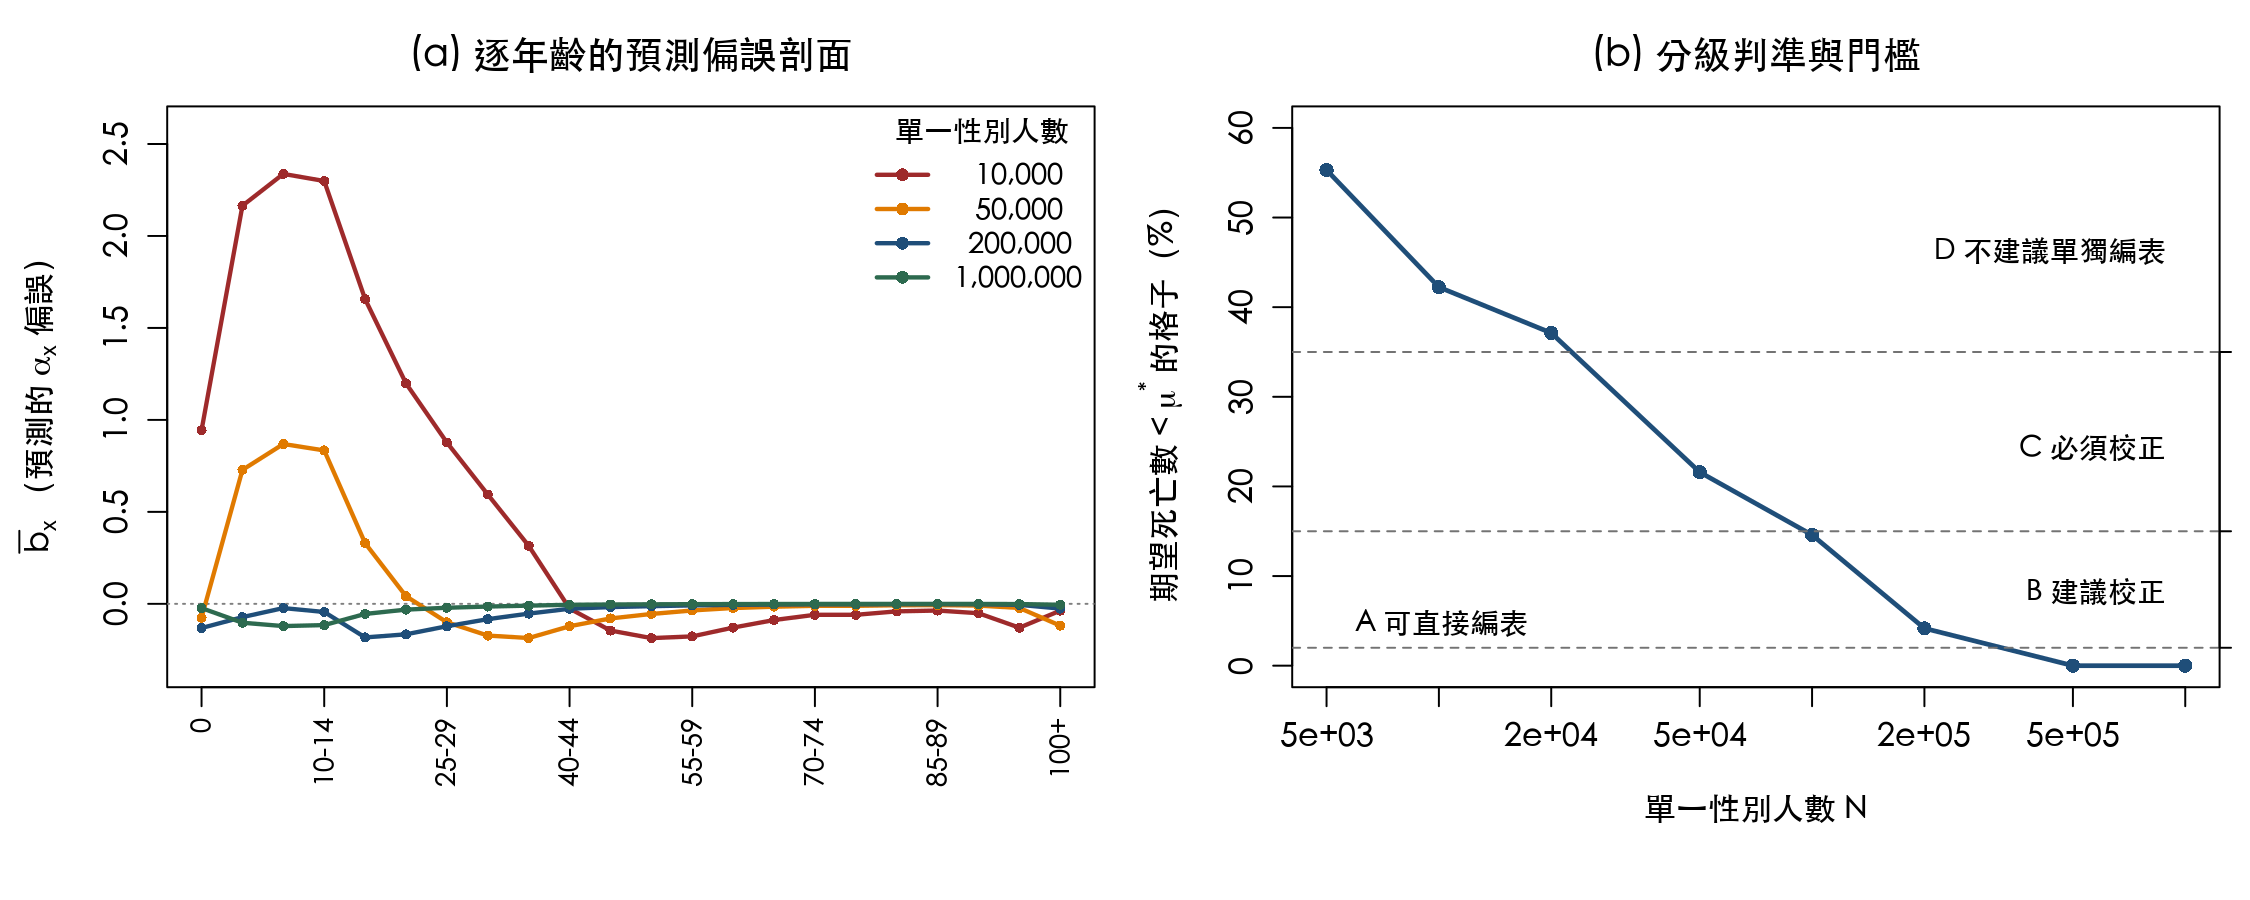
\includegraphics[width=\textwidth]{figF1_feasibility.png}
\caption{事前可行性檢定的輸出}

{\footnotesize 註：(a) 四個人口規模下逐年齡的預測偏誤 $\bar b_x$；(b) 分級判準（期望死亡數低於 $\mu^\ast$ 的格子比例）隨人口規模的變化與四級門檻。}

\label{fig:feas}
\end{figure}

表~\ref{tab:feas} 與圖~\ref{fig:feas} 的設計是在固定年齡結構下改變人口規模，
以判讀分級隨規模的變化與其主因。
從表中可以看到，預測值與第\ref{sec:empmain}的模擬實測吻合至小數第三位：
人數一萬時預測 $+2.337$ 而模擬所得的標準 Lee-Carter $\alpha$ 最大偏誤為
$2.331$，五萬時預測 $+0.869$ 而模擬為 $0.866$，二十萬時預測 $0.183$ 而模擬為
$0.185$。亦即這個不需要模擬的檢定，其輸出就是模擬會給出的那個數字。
特別明顯的是偏誤的主因在人數十萬與二十萬之間換手：
人數十萬以下由零格高估主導，二十萬以上由 Jensen 低估主導，
而後者在四個數量級的人口規模上幾乎固定在 $-0.19$ 附近，
蓋因年齡剖面上總有某一個年齡的期望死亡數落在 $b$ 取極小的 $\mu=2.2886$ 附近，
隨著人口增加，該年齡只是由幼年往中年移動而已。
這正是分級不以 $\max_x|\bar b_x|$ 為判準的理由：

分級與實際可編表範圍之間另有一段差距；這一項對政策最為重要。
我國 368 個鄉鎮市區中有 217 個（$59\%$）的單一性別人數在兩萬以下、
299 個（$81\%$）少於五萬，
對照上述界線，至少 217 個落在 D 級，而落在 B 級者須有單一性別人數
九萬六千以上，亦即總人口約十九萬以上，全國僅少數市區達到。
至於 A 級所需的二十一萬五千，我國只有極少數的市區接近。
誠實的推論是：本文把可用的範圍往下推了，但並未移除下限，
而臺灣多數鄉鎮市區仍在下限之下。
總結以上，表~\ref{tab:feas} 所表現的是一條可以事前判斷、
且與模擬結果一致的分級界線；其政策意涵不是「小區域生命表可以編了」，
而是\textbf{小區域生命表不應一律編製，而應依可行性分級}：
A 與 B 級直接編或加校正編，C 級須校正並揭露不確定性，
D 級不單獨編表而改以合併鄰近地區、多母體共同因子模型，
或只報告年齡標準化的彙總指標。
這正是官方生命表只編到縣市層級的統計依據；本文把那條線量化了。

\subsection{兩個門檻的實務用途與替代值 $c_0$ 的揭露}\label{subsec:thresholds}\label{subsec:c0disc}

第\ref{sec:method}節所導出的兩個門檻，在這個檢定中各有不同的用途，
而兩者的性質相反，須分別陳述。
$\mu^{\ast}=0.9234$ 是偏誤的變號點，用以判斷某一年齡的死亡率被高估或被低估。
它\textbf{由分析者決定}，隨 $c_0$ 移動（第\ref{subsec:bprops}表~\ref{tab:c0shift}）。
在檢定中它決定了表~\ref{tab:feas} 第二欄的「低於 $\mu^{\ast}$ 的格子」，
亦即被高估的格子佔多少。

$\ln2=0.6931$ 是中位數類估計量的崩潰門檻，用以判斷分位數型的穩健方法
是否可用。它\textbf{由資料決定}，不隨 $c_0$ 變動。
此一門檻有一項立即的實務價值：它是對分位數型方法的明確禁區。
實測 1 至 4 歲組的零格比例為 $74\%$，已遠超過 $50\%$
（第\ref{subsec:mixrep}），於是在小人口的幼年組，
以樣本分位數為基礎的估計量不適用，且該限制不是調整參數可以緩解的。
此處須把該上界所涵蓋的範圍寫準：$50\%$ 是中位數這一類\textbf{以樣本分位數
定義}的估計量其崩潰點的上界，因此上述結論直接適用於中位數型 Lee-Carter 與
$\tau$ 固定的分位數迴歸；至於 $c$ 有限的 M-分位數，其崩潰點須另行計算，
本文未作此推導，只能說它在零格比例超過一半的年齡失去了「污染為少數」
這個設計前提。
近年把分位數迴歸引入死亡率模型是一個活躍的方向（\citealp{santolino2020}），
而這個門檻界定了它在小人口上的適用範圍。


檢定的輸出依賴 $c_0$，而 $c_0$ 是分析慣例而非資料。
第\ref{subsec:bprops}的表~\ref{tab:c0shift} 已顯示
$c_0=0.1/0.3/0.5/1.0$ 分別使變號點移至 $0.134/0.533/0.923/1.509$，
亦即同一個年齡在兩家機構的計算中可能一邊被判為高估、另一邊被判為低估。
第\ref{sec:logzero}已把這一點接到 \citet{chenroth2024} 的單位依賴結論上，
此處只把它翻成三條可執行的要求。

首先，費率表與生命表的技術文件應揭露所採的 $c_0$，
其地位與揭露所採的生命表基準年相同。
再來，同業比較與監理審查在比對兩份年齡別死亡率之前，應先確認 $c_0$ 一致，
否則兩表的偏誤方向可能相反而不可直接比較。
最後，較佳的作法是不要依賴 $c_0$：改以 Poisson 直接在計數尺度上配適
（\citealp{brouhns2002}），或以參考母體的標準化死亡比填補零格
（第\ref{sec:smr}），兩者都不需要這個慣例。
本節的檢定指出校正在何時是必要的，下一節構造該校正。

\partline{二}{偏誤的校正}

\section{校正的設計}\label{sec:corr}

\subsection{修改後的估計流程，及其與既有修正方法的關係}\label{subsec:procedure}\label{subsec:relation}

式~\eqref{eq:center} 的中心化在實作上是扣除\textbf{格}而非校正參數，
使校正同時流入三個參數。困難在於 $b$ 依賴未知的 $\mu_{x,t}$，因此須迭代：
實作上先以標準 Lee-Carter 起始，得到一組
$(\hat{\boldsymbol\alpha},\hat{\boldsymbol\beta},\hat{\boldsymbol\kappa})$，
據以算出各格的期望死亡數
$\hat\mu_{x,t}=E_{x,t}\exp(\hat\alpha_x+\hat\beta_x\hat\kappa_t)$；
再以 $\ell_{x,t}-b(\hat\mu_{x,t};c_0)$ 取代原始的 $\ell_{x,t}$，
依式~\eqref{eq:svd} 重新配適，得到新的一組參數後回頭更新 $\hat\mu_{x,t}$，
如此反覆至參數的變動小於容忍值為止，實測收斂約需三至六次。
此一疊代與 \citet{kosmidis2010} 的通用演算法同型。該演算法所要求的輸入是
首階偏誤的\textbf{閉式}，其每一步等於先做一次概似的更新、
再扣除以當前參數估得的偏誤；而因省略了偏誤對參數的導數項，
其收斂速率一般為線性而非二次。本文的兩項輸入皆齊備：
$b(\mu;c_0)$ 由 $D$ 的邊際分布算得（式~\eqref{eq:bform}），
其對 $\mu$ 的導數另有精確式（Proposition~\ref{prop:bp}）；
而實測所需的三至六次疊代與線性收斂的速率相符。
兩者的差別只在所扣除的對象：後者扣的是最大概似估計量的 $O(n^{-1})$ 偏誤，
於是須概似存在；本文扣的是對數轉換與零格替代所造成的偏誤，因此不須。
此一迭代之所以必要，是因為式~\eqref{eq:bform} 依賴未知的 $\mu_{x,t}$，
而後者只能由配適值估計；也正因為如此，$\hat\mu$ 的誤差會隨校正一併注入
每一格，構成第\ref{sec:lim}所述的代價之一。

此一流程與偏誤減少文獻的關係如下。\citet{firth1993} 把偏誤減少方法分為
\textbf{事後修正}（先算最大概似估計值再扣除偏誤的估計，
即 \citealp{coxsnell1968}）與\textbf{預先修正}（修改估計方程本身，
即 \citealp{firth1993} 的 Jeffreys 懲罰）。本文屬前者，但施加對象不同，
而這個不同是決定性的：Cox--Snell 修正的是最大概似估計量的 $O(n^{-1})$
偏誤，前提是最大概似估計值\textbf{存在且有限}；而小人口 Lee-Carter 的核心困難
正是零格導致的完全分離\citep{albert1984}，
Poisson 最大概似的 $\hat\alpha_x$ 可為 $-\infty$（實測人數一萬時
5 至 9 歲組為 $-13.03$），因此 Cox--Snell 在此無從施加。
式~\eqref{eq:bform} 則完全不涉及最大概似估計量，只用到 $D$ 的邊際分布。


另須把本文的校正放回式~\eqref{eq:general} 的分類中，以釐清它與既有補救的
關係。先把該式的損失函數寫清楚。M-分位數的損失為
\begin{equation}\label{eq:mq}
\rho_{\tau,c}(u)=2\,w_\tau(u)\,\psi_c(u),\qquad
w_\tau(u)=\begin{cases}\tau & u>0\\ 1-\tau & u\le 0\end{cases},\qquad
\psi_c(u)=\begin{cases}u^2/2 & |u|\le c\\ c|u|-c^2/2 & |u|>c,\end{cases}
\end{equation}
其中 $\tau$ 控制非對稱、$c$ 控制穩健程度。其兩個極限可直接驗證：
$c\to\infty$ 時 $\psi_c(u)=u^2/2$ 對所有 $u$ 成立，於是
$\rho_{\tau,c}(u)=w_\tau(u)u^2$，即 \citet{newey1987}的非對稱
最小平方，而 $\tau=0.5$ 時 $w_\tau\equiv0.5$，$\rho$ 退化為 $u^2/2$；
$c\to0$ 時 $\psi_c(u)\to c|u|$，因此 $\rho_{\tau,c}(u)\to 2c\,w_\tau(u)|u|$，
而 $w_\tau(u)|u|=u\{\tau-\mathbf{1}(u<0)\}$ 恰為 \citet{koenker1978}
的檢查函數，常數 $2c$ 不影響極小值的位置。
把 $\tau=0.5$、$c=\infty$、$w\equiv1$、$\lambda=0$ 代入式~\eqref{eq:general}
即得式~\eqref{eq:lcobj}，標準 Lee-Carter 因此是該族的一個角落。

由此角落出發，小人口的各種補救各自改動了其中一項設定：把 $c$ 調成有限或把
$\tau$ 調離 $0.5$ 即得穩健損失；把 $w$ 取為 $\hat\mu$ 即得資訊加權；
把 $\lambda$ 調離零即得 Ridge、LASSO 或經驗貝氏收縮。
此處須確立的是這三者與本文的中心化之間的關係。

關鍵的觀察是三項設定都不改變母體估計方程在真值處的值。就損失形狀而言，
把 $\psi$ 換成 $\psi_{\tau,c}=\rho_{\tau,c}'$ 之後，母體估計方程變為
$\Ex[\psi_{\tau,c}(u(\theta_0))]$，其值一般\textbf{仍不為零}，事實上因 $\psi_{\tau,c}$ 非線性，該值與 $b$ 的關係還更複雜，
於是問題不但沒解決，連「該扣多少」都不再有閉式。就權重而言，
式~\eqref{eq:pop} 在加權後為 $\sum_{x,t}w_{x,t}\Ex[\psi(u_{x,t})]=
\sum_{x,t}w_{x,t}\,b(\mu_{x,t};c_0)$，這是 $b$ 的加權和；
除非權重恰好使該和為零（而那需要事先知道 $b$，即已經做了本文的計算），
否則它同樣不為零。就懲罰而言，$\lambda P(\theta)$ 在解的位置上加一個朝
收縮目標的拉力，這改變的是 $\theta^{\ast}$ 相對於母體估計方程解的位置，
而非母體估計方程本身；它以一個\textbf{新的}偏誤（收縮偏誤）去交換變異數，
並不移除原有的那一項。

三者因此都作用在一個\textbf{已經 Fisher 不一致}的估計方程上，
而式~\eqref{eq:center} 的中心化則直接處理不一致本身。
用式~\eqref{eq:pop} 的語言說，三項設定改變的是估計方程的\textbf{形狀}
（$\psi$）與\textbf{權重}（$w$），中心化改變的是它的\textbf{位置}，
兩者在該式中出現在不同的地方，因此彼此正交。

\subsection{參數偏誤的成分分解}\label{sec:betadec}

Corollary~\ref{cor:alpha} 只涵蓋 $\alpha_x$，因為它在奇異值分解之前即已由
列平均定出。但同一條推導可以再往下走一步，刻畫 $\beta_x$ 與 $\kappa_t$ 所受的影響。
這一步之所以重要，在於本文的標的是 $\alpha_x$ 與 $\beta_x$ 兩者偏誤的同時
降低，而至此只處理了其中一個。
依式~\eqref{eq:svd}，$(\hat{\boldsymbol\beta},\hat{\boldsymbol\kappa})$ 取自
中心化矩陣 $Z_{x,t}=\ell_{x,t}-\hat\alpha_x$ 的第一組奇異向量，
取其期望並利用 $\sum_t\kappa_t=0$，即得：

\begin{prop}\label{prop:beta}
$\displaystyle \Ex[Z_{x,t}]=\beta_x\kappa_t+\Delta_{x,t},\qquad
\Delta_{x,t}=b(\mu_{x,t};c_0)-\bar b_x,\quad
\bar b_x=\frac1T\sum_s b(\mu_{x,s};c_0).$
\end{prop}

亦即期望矩陣\textbf{不是}秩一訊號 $\boldsymbol\beta\boldsymbol\kappa^{\top}$，
而多了一個確定性的擾動 $\Delta$，其內容為 $b$ 在該年齡\textbf{列內隨 $t$
的變動}。此處的結構是：若 $b(\mu_{x,t})$ 在列內不隨 $t$ 變動，
則 $\Delta=0$，$\beta_x$ 完全不受對數偏誤影響，因為列平均已把它吸收進
$\hat\alpha_x$。但死亡率隨年份改善使 $\mu_{x,t}$ 隨 $t$ 下降，
而 $b$ 是 $\mu$ 的非線性函數，於是 $\Delta\ne0$。

由Proposition~\ref{prop:beta} 可把 $\hat\beta$ 的誤差\textbf{精確}分解為兩部分，
不需一階近似：對無噪音的期望矩陣
$\boldsymbol\beta\boldsymbol\kappa^{\top}+\Delta$ 直接作奇異值分解，
所得的 $\hat\beta$ 與真值之差即 $\Delta$ 單獨造成的\textbf{確定性成分}；
以模擬測得的總誤差減去它，即為噪音旋轉奇異向量所造成的\textbf{隨機成分}。
表~\ref{tab:betadec} 給出結果。

\begin{table}[H]
\centering
\caption{$\alpha$、$\beta$ 與漂移項的確定性／隨機成分分解（標準 Lee-Carter）}
\small
\begin{tabular}{lrrrr}
\toprule
 & $N=10^4$ & $N=5\times10^4$ & $N=2\times10^5$ & $N=10^6$\\
\midrule
$\|\Delta\|_F/\|\boldsymbol\beta\boldsymbol\kappa^{\top}\|_F$
 & 0.693 & 0.499 & 0.189 & 0.064\\
\midrule
$\alpha$ 最大偏誤：確定性 $|\bar b_x|$ & 2.337 & 0.869 & 0.183 & 0.121\\
$\alpha$ 最大偏誤：模擬總量 & 2.331 & 0.895 & 0.296 & 0.212\\
\quad 確定性佔比 & \textbf{100\%} & \textbf{97\%} & 62\% & 57\%\\
\midrule
SSE($\beta$)：確定性 & 0.731 & 0.256 & 0.032 & 0.002\\
SSE($\beta$)：模擬總量 & 7.916 & 4.449 & 1.400 & 0.229\\
\quad 確定性佔比 & \textbf{9.2\%} & \textbf{5.8\%} & 2.3\% & 1.0\%\\
\midrule
漂移偏誤：確定性 & 0.178 & 0.102 & 0.018 & $-0.013$\\
漂移偏誤：模擬總量 & 0.344 & 0.334 & 0.212 & 0.044\\
\quad 確定性佔比 & \textbf{52\%} & 30\% & 8.6\% & ---\\
\bottomrule
\end{tabular}
\label{tab:betadec}
\end{table}

表~\ref{tab:betadec} 是本文對偏誤可否降低這一課題的核心結果，
而三個參數給出的答案並不相同。先看 $\alpha_x$：人數一萬時確定性成分
$2.337$ 與模擬總量 $2.331$ 幾乎相同、佔 $100\%$，人數五萬時為 $97\%$，
這說明了中心化對它有效的原因，所移除的正是全部的偏誤；人數增大後佔比
降至六成，是因為此時絕對偏誤已小，隨機成分的相對重要性隨之上升。
$\beta_x$ 則相反，確定性成分在四個規模下分別只佔總誤差的 $9.2\%$、
$5.8\%$、$2.3\%$、$1.0\%$，其餘九成以上來自異質變異的噪音旋轉主奇異向量，
即各列噪音變異數不同時樣本 Gram 矩陣的對角線被不均勻地灌水，
主向量因此被系統性旋轉。此一機制與 $b$ 無關，因此無論把 $b$ 算得多準
都無法處理它。這是一個否定的結論，但它是有內容的否定：它指出 $\beta_x$
的補救必須改換工具，而正確的工具是加權，若各格的權重使噪音變異數大致
相等，則該旋轉在一階上消失，第\ref{sec:result}節的實測證實了這一點。
漂移項介於兩者之間且轉變得很快，人數一萬時確定性成分佔 $52\%$、
五萬時 $30\%$、二十萬時僅 $8.6\%$；於是在極小人口下校正對它理論上應有
一半的改善空間，但第\ref{sec:result}節將顯示實測並未實現，
因為校正須以 $\hat\mu$ 代入，而 $\hat\mu$ 的誤差所注入的噪音恰好抵銷了
這部分的收益。

表~\ref{tab:betadec} 的數字可以畫成圖，而圖比表更能顯示兩個參數差別的所在。圖~\ref{fig:bband} 把 $\beta_x$ 各估計量的重複分布畫出來，
與圖~\ref{fig:aband} 的 $\alpha_x$ 恰成對照：後者的帶窄而整條偏離真值，
偏誤是主角；前者的帶寬而大致罩住真值，變異數才是主角。
兩張圖並列，等於把表~\ref{tab:betadec} 的確定性佔比由數字翻譯成形狀，佔比高者表現為「帶窄而偏移」，佔比低者表現為「帶寬而居中」。

\begin{figure}[H]
\centering
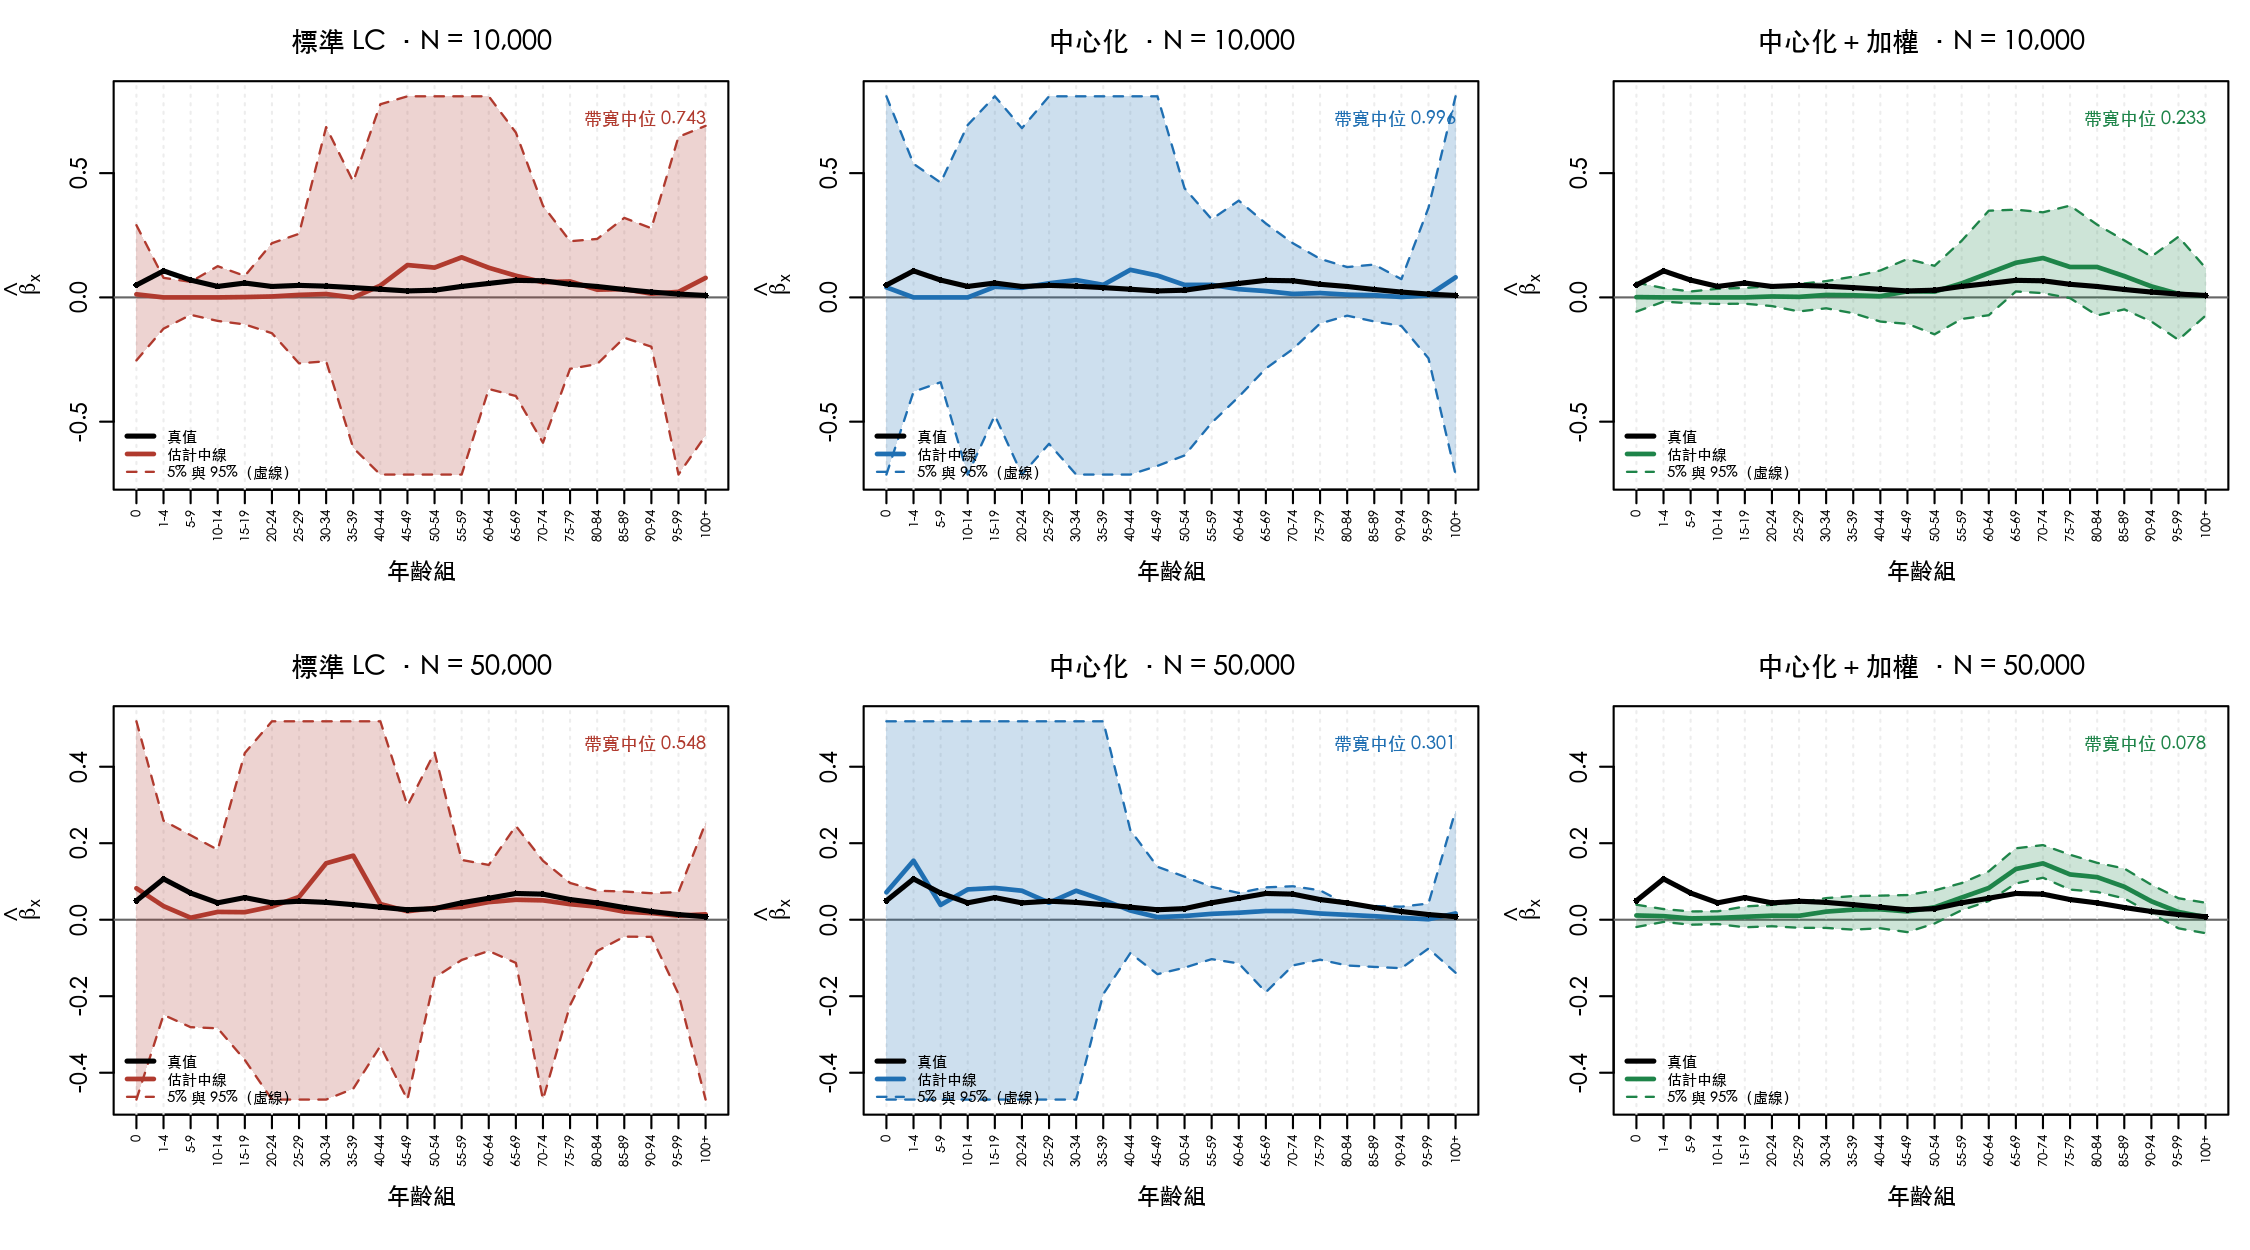
\includegraphics[width=\textwidth]{figT2_beta_band.png}
\caption{$\hat\beta_x$ 的 5--95\% 帶（上列人數一萬、下列人數五萬）}

{\footnotesize 註：每格一個估計量，黑線為真值。}

\label{fig:bband}
\end{figure}

兩圖並列即本文的核心對照。$\alpha_x$ 的帶窄而偏離真值，
$\beta_x$ 的帶寬而大致罩住真值：人數五萬時 $\alpha$ 的最大偏誤 $0.866$
是其帶寬 $0.218$ 的\textbf{四倍}，而 $\beta$ 的中線離真值中位僅 $0.011$、
帶寬卻達 $0.548$，相差\textbf{五十倍}。這兩個比值正是
表~\ref{tab:betadec} 確定性佔比（$97\%$ 對 $5.8\%$）的另一種表達，
也說明了同一個校正對兩者效果截然不同的原因。

圖~\ref{fig:bband} 另顯示兩項須一併記載的結果。一方面，中心化單獨使用時
$\beta$ 的帶反而變寬（人數一萬時 $0.743\to0.996$），視覺上比
表~\ref{tab:estcmp} 的 SSE 數字更直接，校正所注入的 $\hat\mu$ 噪音
在 $\beta$ 上是淨損失。另一方面，中心化加上加權雖使帶寬大幅收窄
（人數五萬時 $0.548\to0.078$，七倍），但其中線在 60 至 85 歲一段
明顯高於真值（中線離真值的中位由 $0.011$ 升至 $0.036$），
亦即它是以\textbf{偏誤換變異數}，而非同時改善兩者。
相較之下 Firth 在人數五萬時的帶寬為 $0.153$、中線離真值僅 $0.003$，
兩者兼得，這也是第\ref{sec:result}節中 Firth 在多數指標上仍勝出的原因。

綜合上述，偏誤在特定假設下可否降低，其結論可寫成兩個條件式，
而兩者互不涵蓋。
首先，若\textbf{Poisson 假設成立}，則 $\alpha_x$ 的偏誤可由式~\eqref{eq:bform}
算出並扣除，改善幅度由表~\ref{tab:betadec} 的確定性佔比給出上界
（人數一萬與五萬時接近全部）。此外，若\textbf{加權後各格的噪音變異數
大致相等}，則 $\beta_x$ 與漂移項的隨機成分可在一階上移除；
但此條件無法由本文的閉式提供，須另行處理。兩個條件互不涵蓋，
這也是小人口 Lee-Carter 需要兩種藥的原因。


\section{實證結果}\label{sec:result}

\subsection{整體指標的比較}\label{sec:empmain}

以下的比較採與第\ref{sec:valid}節完全相同的亂數種子，因此各表可逐格對照。
四張表比較的是同一組估計量，各自加入一個維度：表~\ref{tab:betadec} 把誤差
拆成確定性與隨機成分，說明兩個參數為何需要不同的工具；
表~\ref{tab:estcmp} 比較參數層次的三項指標；
表~\ref{tab:e0var} 把參數的改善翻成使用者真正關心的量；
表~\ref{tab:real} 則在真實資料上重做表~\ref{tab:estcmp}，
以分離「模型正確時的表現」與「模型誤設所造成的損失」。
所比較的五個估計量分別對應文獻所記載的三項限制：標準 Lee-Carter 為未修正的基準，
Poisson 最大概似用以呈現事後修正所須的「最大概似估計值存在」在本問題上的
後果，Firth 代表預先修正一路，
中心化與中心化加權則為本文所提的修正。

\begin{table}[H]
\centering
\caption{中心化與既有作法的比較（重複 100 次，取中位數）}
\small
\begin{tabular}{llrrrrr}
\toprule
$N$ & 估計量 & $\alpha$ 中位 & $\alpha$ 最大 & SSE($\beta$) & cor($\beta$) & 漂移偏誤\\
\midrule
\multirow{5}{*}{$10^4$}
 & 標準 Lee-Carter          & 0.1612 & 2.3309 & 7.916 & $-0.074$ & 0.3436\\
 & Poisson MLE       & 0.0495 & 13.0317 & 15.525 & 0.118 & 0.1612\\
 & Firth            & \textbf{0.0248} & \textbf{0.4267} & 17.797 & 0.116 & 0.2237\\
 & 中心化           & 0.0693 & 0.5008 & 18.048 & $-0.078$ & 0.3544\\
 & 中心化 $+$ 加權   & 0.1749 & 0.7399 & \textbf{2.537} & 0.111 & \textbf{0.1884}\\
\midrule
\multirow{5}{*}{$5\times10^4$}
 & 標準 Lee-Carter          & 0.0611 & 0.8658 & 4.449 & 0.037 & 0.3339\\
 & Poisson MLE       & 0.0073 & 0.2260 & 1.756 & 0.365 & 0.0492\\
 & Firth            & 0.0088 & \textbf{0.0680} & 1.410 & \textbf{0.397} & \textbf{0.0485}\\
 & 中心化           & \textbf{0.0093} & 0.2434 & 8.834 & 0.198 & 0.3335\\
 & 中心化 $+$ 加權   & 0.0110 & 0.2524 & \textbf{1.023} & 0.179 & 0.1381\\
\midrule
\multirow{5}{*}{$2\times10^5$}
 & 標準 Lee-Carter          & 0.0231 & 0.1846 & 1.400 & 0.379 & 0.2117\\
 & Poisson MLE       & \textbf{0.0018} & 0.0361 & 0.346 & 0.596 & 0.0267\\
 & Firth            & 0.0025 & \textbf{0.0398} & \textbf{0.333} & \textbf{0.605} & \textbf{0.0262}\\
 & 中心化           & 0.0032 & 0.1778 & 3.499 & 0.438 & 0.2747\\
 & 中心化 $+$ 加權   & 0.0071 & 0.2897 & 0.832 & 0.213 & 0.1106\\
\bottomrule
\end{tabular}
\label{tab:estcmp}
\end{table}

圖~\ref{fig:cmp} 與圖~\ref{fig:e0} 把表~\ref{tab:estcmp} 與
表~\ref{tab:real} 的內容畫出來，前者比較三項參數指標、後者直接看使用者
真正關心的平均餘命。

\begin{figure}[H]
\centering
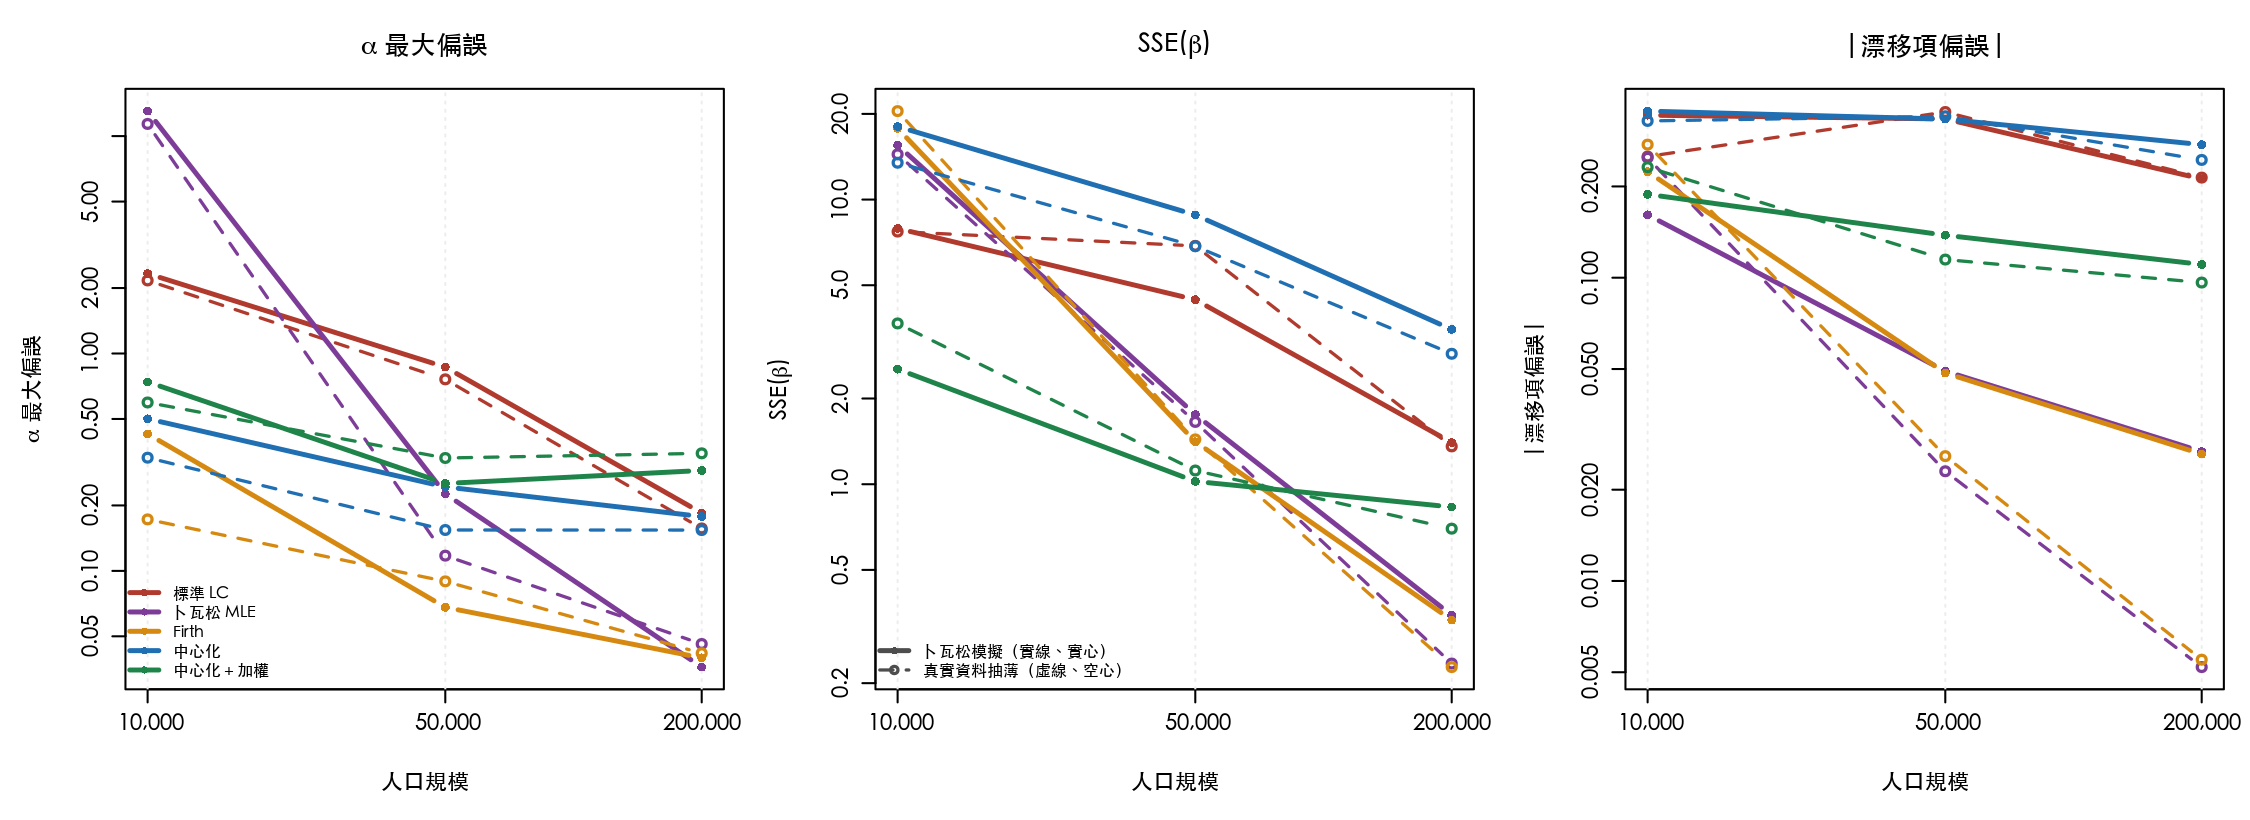
\includegraphics[width=\textwidth]{figT3_estimator_compare.png}
\caption{三項指標隨人口規模的變化（縱軸取對數）}

{\footnotesize 註：實線與實心點為 Poisson 模擬，虛線與空心點為實際觀測死亡數的 Poisson 抽薄。}

\label{fig:cmp}
\end{figure}

\begin{figure}[H]
\centering
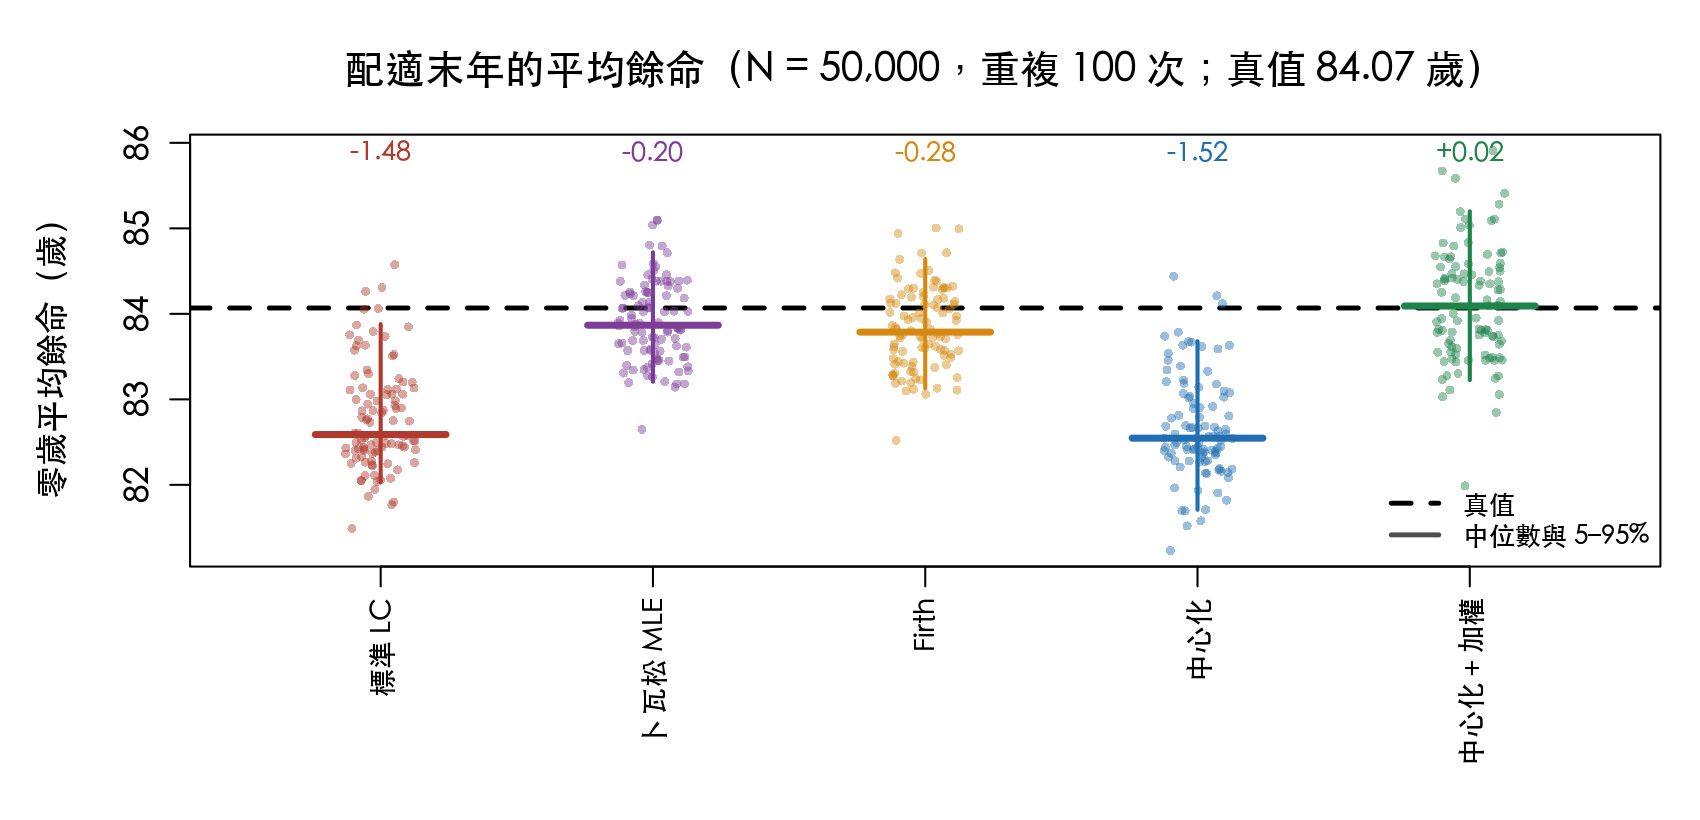
\includegraphics[width=0.78\textwidth]{figT4_e0_by_estimator.png}
\caption{配適末年零歲平均餘命的 100 次重複（人數五萬）}

{\footnotesize 註：虛線為真值 $84.07$ 歲，各估計量上方標示其中位偏誤。}

\label{fig:e0}
\end{figure}

圖~\ref{fig:cmp} 顯示一項須並列才能辨識的訊息：實線與虛線幾乎平行，
亦即以真實觀測死亡數抽薄所得的結論與純 Poisson 模擬一致；
唯一的例外是標準 Lee-Carter 的 SSE($\beta$)，其虛線明顯高於實線，
這正是第\ref{sec:real}所述「真實資料中不合秩一結構的成分也被 $\hat\beta$
吸收」的表現。圖~\ref{fig:e0} 則把參數層次的改善翻譯成使用者真正關心的量：
標準 Lee-Carter 的一百次重複全部落在真值之下，中位數低估 $1.48$ 歲；
Poisson 最大概似與 Firth 分別改善至 $-0.20$ 與 $-0.28$ 歲；
而中心化加權的中位數為 $+0.02$ 歲，點雲已大致對稱地分布在真值兩側。

第\ref{sec:method}節末所提的兩項預測都成立；其中後者的成立方式比前者
更有說服力。前一項預測是中心化應大幅移除 $\alpha_x$ 的偏誤：
$\alpha$ 偏誤中位數在三個規模下分別下降 $2.3$、
$6.6$、$7.2$ 倍；人數一萬時 $\alpha$ 最大偏誤由 $2.3309$ 降至 $0.5008$，
且決定性地優於 Poisson 最大概似的 $13.03$，後者因完全分離而崩壞，
這正是式~\eqref{eq:bform} 不依賴最大概似這個性質的價值。
加上資訊加權之後，該估計量在三個規模的每一項指標上都優於標準 Lee-Carter
（$\beta$ 的平方誤差和 $7.92\to2.54$、$4.45\to1.02$、$1.40\to0.83$；
漂移項偏誤 $0.34\to0.19$、$0.33\to0.14$、$0.21\to0.11$），
且完全留在奇異值分解的架構內、沒有調校參數。

後一項是反向的預測：中心化動的是估計方程的中心，而漂移項的誤差來自權重，
故中心化\textbf{不應}改善漂移項。漂移項偏誤由 $0.3436$、$0.3339$、$0.2117$
變為 $0.3544$、$0.3335$、$0.2747$，即未改善。
此一預測有風險——若偏誤的來源不是推導所描述的那一個，
漂移項沒有理由恰好不動——故其成立比正向預測更具證據力，
但它所支持的是「與推導相容」而非「推導已被證明」。
既然一個確定性的 $\mu$ 函數可以移除 $\alpha$ 的偏誤卻完全不動漂移項，
漂移項的偏誤就不可能是對數轉換造成的，它須以權重 $w$ 處理，
此即「中心化 $+$ 加權」一列改善漂移項的原因。

\subsection{逐年齡的誤差剖面}\label{sec:ageprof}

前一小節的指標是跨年齡彙總的。但閉式 $b(\mu;c_0)$ 是期望死亡數的函數，
而期望死亡數在年齡之間相差三個數量級，
因此閉式對改善的\textbf{分布}也給出預測：
校正的效果應集中在死亡數少的年齡，在死亡數多的年齡則幾乎沒有改善空間，
因為該處 $b(\mu)\approx-1/(2\mu)$ 本就接近零。
本小節把誤差拆到年齡維度，既是呈現上的細緻化，也是對推導的另一次檢驗。

\begin{table}[H]
\centering
\caption{逐年齡段的均方根誤差與各段的平均期望死亡數（人數五萬，重複 100 次）}
\small
\renewcommand{\arraystretch}{1.1}
\begin{tabular}{lrrrrrr}
\toprule
 & 平均期望 & \multicolumn{3}{c}{$\alpha_x$ 的均方根誤差} & \multicolumn{2}{c}{$\beta_x$ 的均方根誤差}\\
\cmidrule(lr){3-5}\cmidrule(lr){6-7}
年齡段 & 死亡數 & 標準 Lee-Carter & 僅校正 $\alpha$ & ＋加權 & 標準 Lee-Carter & ＋加權\\
\midrule
$0$--$14$ 歲   & 0.50  & 0.6452 & \textbf{0.3480} & 0.3493 & 0.8718 & \textbf{0.0640}\\
$15$--$34$ 歲  & 1.10  & 0.2126 & 0.2164 & 0.2162 & 1.4456 & \textbf{0.0427}\\
$35$--$59$ 歲  & 8.03  & 0.1307 & 0.0872 & \textbf{0.0837} & 0.7645 & \textbf{0.0286}\\
$60$--$84$ 歲  & 44.41 & 0.0357 & \textbf{0.0317} & 0.0626 & 0.2658 & 0.0725\\
$85$ 歲以上    & 39.03 & 0.0677 & \textbf{0.0483} & 0.0506 & 0.2970 & \textbf{0.0370}\\
\bottomrule
\end{tabular}
\label{tab:ageband}
\end{table}

\begin{figure}[H]
\centering
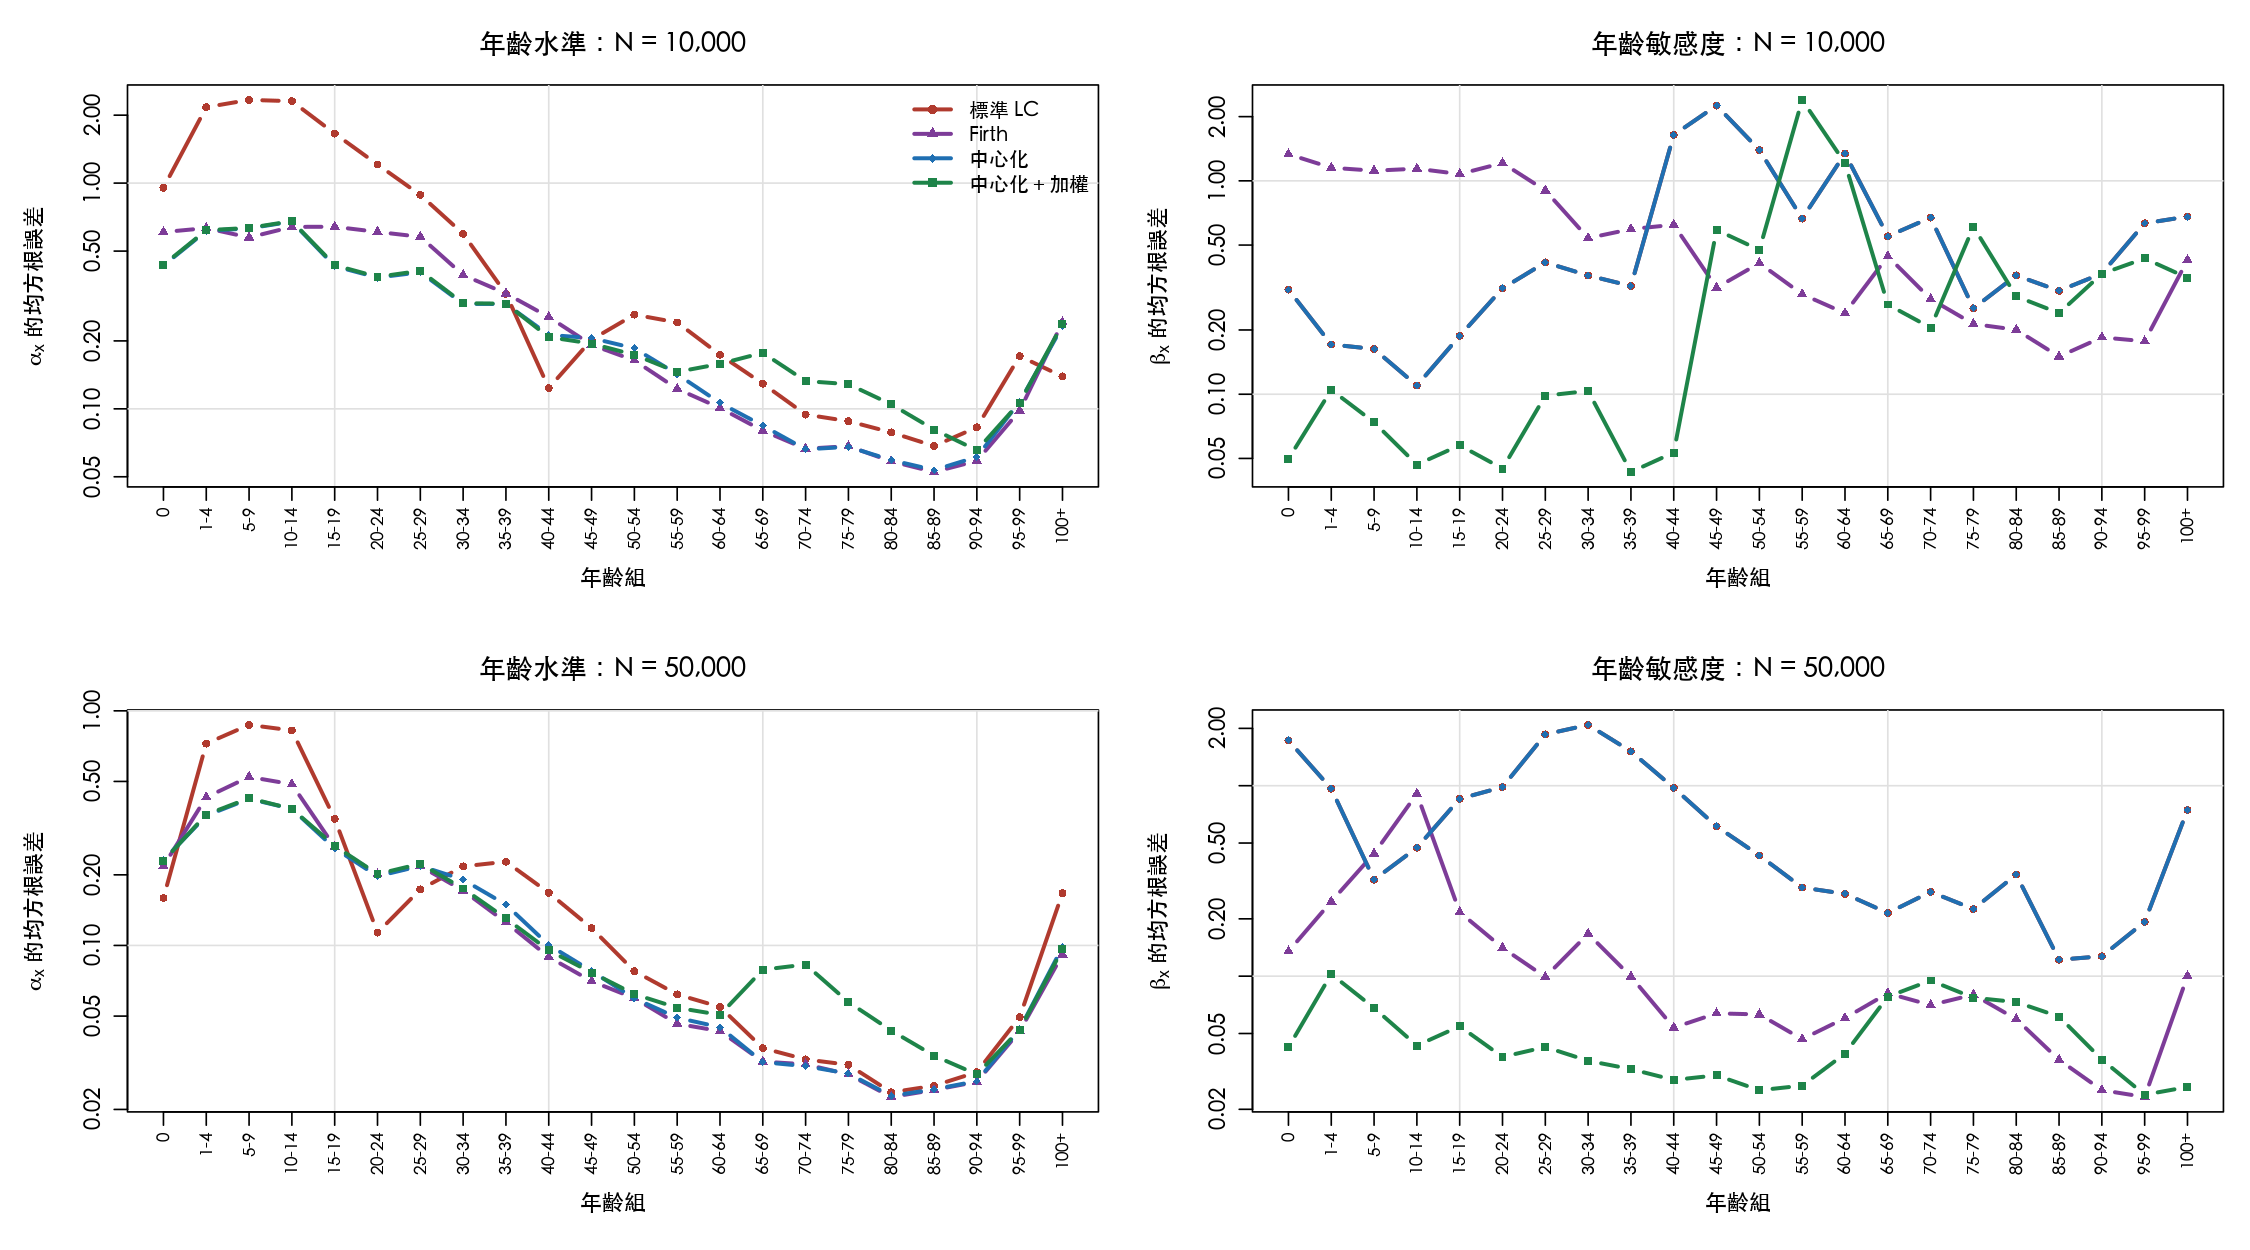
\includegraphics[width=\textwidth]{figT9_age_profile.png}
\caption{逐年齡的均方根誤差（縱軸取對數）}

{\footnotesize 註：上列為人數一萬、下列為人數五萬；左欄為 $\alpha_x$、右欄為 $\beta_x$。右欄中標準 Lee-Carter（紅）的線完全被中心化（藍）覆蓋，因為僅校正 $\alpha_x$ 不改變中心化矩陣。}

\label{fig:ageprof}
\end{figure}

$\alpha_x$ 的改善集中在死亡數少的年齡。
人數五萬時 $0$ 至 $14$ 歲組的平均期望死亡數僅 $0.50$ 人，
其均方根誤差由 $0.645$ 降至 $0.348$，改善近一倍；
而 $60$ 至 $84$ 歲組的平均期望死亡數達 $44$ 人，標準 Lee-Carter 的誤差本就只有
$0.036$，校正後為 $0.032$。人數一萬時的對比更明顯：
$0$ 至 $14$ 歲組由 $1.942$ 降至 $0.588$，$15$ 至 $34$ 歲組由 $1.088$ 降至
$0.376$，而 $60$ 歲以上兩組的改善倍數皆在 $1$ 附近。
改善的分布與 $b(\mu)$ 的形狀一一對應，蓋因所扣除的量本來就是 $b(\mu)$，
而該函數在 $\mu$ 小處趨於 $\log(c_0/\mu)$、在 $\mu$ 大處只有 $-1/(2\mu)$。
這一點是第\ref{sec:valid}節的驗證在年齡維度上的細部版本。

$\beta_x$ 的情形則相反，改善遍及全部年齡，且幅度遠大於 $\alpha$，
人數五萬時五個年齡段的改善倍數分別為 $13.6$、$33.9$、$26.7$、$3.7$、$8.0$ 倍。
兩者的差異可由第\ref{sec:betadec}的分解解釋：
$\alpha$ 的誤差幾乎全為確定性，只能由扣除 $b$ 改善，改善的量即為 $b$ 本身，
於是隨年齡而異；$\beta$ 的誤差九成以上為隨機，其來源是各格變異數的異質，
因此由加權處理，而加權對所有年齡同時生效。
表中「僅校正 $\alpha$」一欄的 $\beta$ 誤差與標準 Lee-Carter 完全相同
（五個年齡段分別為 $0.8718$、$1.4456$、$0.7645$、$0.2658$、$0.2970$），
此一逐位相同的結果在數值上確認了式~\eqref{eq:svd} 的性質：
$\hat\alpha_x$ 在奇異值分解之前定出，事後扣除 $\bar b_x$ 不動中心化矩陣，
因此完全不影響 $\hat\beta_x$，兩項改善可以疊加的理由至此得到逐年齡的驗證。

改善有限的年齡段有兩處；兩者的性質不同。
$15$ 至 $34$ 歲組的 $\alpha$ 沒有改善（$0.213$ 對 $0.216$），
這一段屬於可預期的無改善：該年齡段的平均期望死亡數為 $1.10$，
恰落在變號點 $\mu^{\ast}=0.9234$ 附近，由第\ref{subsec:bprops}
$b(\mu^{\ast})=0$，亦即該處本就沒有偏誤可扣，誤差幾乎全為變異數。
變號點的位置由閉式事先算出，而實測的無改善帶恰好落在該處，
於是這不是方法的缺陷，反而是閉式的另一項獨立驗證。
$60$ 至 $84$ 歲組則不同，該段在加上資訊加權後由 $0.032$ 惡化為 $0.063$。
表中「僅校正 $\alpha$」與「＋加權」兩欄的對比顯示問題出在加權而非中心化，
單純中心化在該段仍優於標準 Lee-Carter（$0.0317$ 對 $0.0357$）。
蓋因加權版的 $\hat\alpha_x$ 取的是以 $\hat\mu_{x,t}$ 為權重的加權列平均，
而非式~\eqref{eq:svd} 的等權列平均，在死亡數多、各年變異已經很小的年齡，
加權只是把某些年份的觀測放大，反而引入額外的變異。
這是本文設計上的一項限制，而且是可以修補的限制：
權重只需施加於 $\beta$ 與 $\kappa$ 的求解，$\alpha$ 仍取等權列平均即可。
本文尚未實作該版本，列為後續工作。

這組表與圖所呈現的是誤差的兩種來源在年齡上有不同的分布：
$\alpha$ 的偏誤集中在資訊最少的年齡，因此校正的效果也集中在該處；
$\beta$ 的誤差來自變異的異質，因此加權的效果遍及全齡。
兩者合起來，使所提的修正在死亡數少的年齡改善最大，
而這正是小人口編表最困難的部分。

\subsection{平均餘命的偏誤與離散}\label{sec:e0var}

前一小節的比較以中位偏誤為主，但偏誤只是估計誤差的一半。
所提的修正只改變估計方程的中心，理論上不應改變其變異數；
這是一個可檢驗的陳述，而檢驗它的地方正是使用者真正關心的標的量。
本小節於是把配適末年零歲平均餘命的 100 次重複分布完整列出，
並一併檢驗一項相關的性質：死亡率在小人口下的劇烈震盪眾所周知，
而平均餘命作為整條死亡率曲線的加權平均，其震盪的程度尚未見記載。

\begin{table}[H]
\centering
\caption{配適末年零歲平均餘命的偏誤與離散（重複 100 次，單位：歲）}
\small
\renewcommand{\arraystretch}{1.1}
\begin{tabular}{llrrrrrr}
\toprule
$N$ & 估計量 & 中位偏誤 & 標準差 & 四分位距 & 全距 & 均方根誤差 & 命中率\\
\midrule
\multirow{6}{*}{$10^4$}
 & 標準 Lee-Carter             & $-3.621$ & \textbf{0.945} & \textbf{1.317} & \textbf{4.636} & 3.557 & 0.00\\
 & Poisson MLE          & \textbf{$-0.820$} & 1.155 & 1.438 & 7.646 & \textbf{1.378} & \textbf{0.33}\\
 & Firth               & $-1.327$ & 1.117 & 1.328 & 7.859 & 1.728 & 0.18\\
 & 中心化              & $-1.717$ & 0.880 & 0.985 & 4.232 & 1.775 & 0.08\\
 & 中心化＋加權        & $-1.104$ & 1.639 & 2.368 & 7.671 & 1.915 & 0.17\\
 & 僅校正 $\alpha$＋加權 & $-1.088$ & 1.470 & 2.088 & 7.282 & 1.807 & 0.21\\
\midrule
\multirow{6}{*}{$5\times10^4$}
 & 標準 Lee-Carter             & $-1.480$ & 0.613 & 0.721 & 3.086 & 1.425 & 0.13\\
 & Poisson MLE          & $-0.202$ & \textbf{0.477} & \textbf{0.683} & \textbf{2.448} & \textbf{0.501} & \textbf{0.67}\\
 & Firth               & $-0.282$ & 0.478 & 0.709 & 2.484 & 0.532 & 0.63\\
 & 中心化              & $-1.522$ & 0.599 & 0.703 & 3.209 & 1.523 & 0.11\\
 & 中心化＋加權        & $+0.023$ & 0.670 & 0.933 & 3.921 & 0.668 & 0.53\\
 & 僅校正 $\alpha$＋加權 & \textbf{$+0.007$} & 0.613 & 0.759 & 3.366 & 0.610 & 0.58\\
\midrule
\multirow{6}{*}{$2\times10^5$}
 & 標準 Lee-Carter             & $-0.899$ & 0.634 & 0.843 & 3.094 & 1.108 & 0.23\\
 & Poisson MLE          & \textbf{$-0.031$} & 0.276 & 0.378 & 1.463 & \textbf{0.276} & 0.92\\
 & Firth               & $-0.050$ & \textbf{0.275} & \textbf{0.377} & \textbf{1.459} & 0.277 & \textbf{0.93}\\
 & 中心化              & $-1.422$ & 0.693 & 0.943 & 3.018 & 1.415 & 0.14\\
 & 中心化＋加權        & $+0.333$ & 0.344 & 0.409 & 1.984 & 0.504 & 0.65\\
 & 僅校正 $\alpha$＋加權 & $+0.167$ & 0.326 & 0.459 & 1.757 & 0.380 & 0.80\\
\bottomrule
\end{tabular}

\vspace{2pt}
\parbox{0.92\textwidth}{\footnotesize 註：命中率為 100 次重複中
$|\hat e_0-e_0|\le0.5$ 歲的比例，真值為 $84.07$ 歲。粗體為該規模下各欄的
最小值；須注意離散三欄的最小值不代表估計較佳，人數一萬時標準 Lee-Carter 的離散最小，
但其中位偏誤達 $-3.621$ 歲。}
\label{tab:e0var}
\end{table}

人數五萬的「僅校正 $\alpha$＋加權」一列最為明顯：
中位偏誤由標準 Lee-Carter 的 $-1.480$ 歲降為 $+0.007$ 歲，
而標準差完全不變（$0.613$ 對 $0.613$）。
這與第\ref{subsec:consistency}的推導吻合。
式~\eqref{eq:center} 的中心化是在估計方程上加一個確定性的位移，
它改變解的位置而不改變解的隨機波動，因此偏誤被移除而離散保持原狀；
均方根誤差隨之由 $1.425$ 降為 $0.610$。
命中率一欄（$|\hat e_0-e_0|\le0.5$ 歲的比例）比均方根誤差更貼近編表者的
需求，而它給出全表最大的對比：人數五萬時由 $0.13$ 升至 $0.58$、
人數二十萬時由 $0.23$ 升至 $0.80$。均方根誤差是統計讀者的語言，
命中率則是編表者的語言，兩者應並列。
就這一點而言，所提的修正與正則化的「以偏誤換變異數」性質不同，
後者是取捨，前者是沒有代價的位移。

逐格校正的版本則須付代價。「中心化＋加權」把 $b(\hat\mu_{x,t})$ 逐格扣除，
因此把 $\hat\mu$ 的估計誤差注入每一格，標準差由 $0.613$ 升至 $0.670$、
四分位距由 $0.721$ 升至 $0.933$。兩個版本的中位偏誤幾乎相同
（$+0.023$ 對 $+0.007$），差別全在離散，
再次確認離散的增加源自逐格代入而非中心化本身。

表中不利於本文的部分在 Firth 一列。人數二十萬時 Firth 的均方根誤差為
$0.277$ 歲，優於本文的 $0.380$；人數五萬時為 $0.532$ 對 $0.610$，亦略優。
原因可由表直接讀出：Firth 的標準差在兩個規模下分別為 $0.275$ 與 $0.478$，
明顯低於本文的 $0.326$ 與 $0.613$。
蓋因預先修正在修正偏誤的同時也收縮了估計量，連帶降低變異數，
而本文的事後扣除完全不動變異數。
這是本文方法的一項界線而非瑕疵，但須明白寫出：
若標的是參數本身，所提的修正較佳（見表~\ref{tab:estcmp} 的
SSE($\beta$) 與第\ref{sec:joint}）；若標的是平均餘命且人數在十萬以上，
Firth 的均方根誤差較小。
人數一萬時兩者皆不理想，Poisson 最大概似的中位偏誤雖最小（$-0.820$），
其全距卻達 $7.65$ 歲，且有 $2\%$ 的重複完全發散，不宜使用；
該規模下所有估計量的命中率都在三分之一以下，
顯示資訊量本身已不足以支持編表。
這張表所呈現的是偏誤與離散在各估計量之間的分工：
所提的修正把中心移到正確的位置而不動離散，Firth 則兩者同時收縮，
於是在以參數為標的時前者較佳，在以平均餘命為標的且人數較多時後者較佳。

\begin{table}[H]
\centering
\caption{零歲平均餘命逐年序列的震盪幅度（100 次重複的中位數，單位：歲）}
\small
\begin{tabular}{llrrr}
\toprule
$N$ & 序列 & 逐年變動均值 & 粗糙度 & 全距\\
\midrule
\multirow{4}{*}{$10^4$}
 & 真值                      & 0.299 & 0.330 & 4.534\\
 & 觀測（零格以 $0.5$ 替代） & \textbf{1.304} & \textbf{2.266} & 6.357\\
 & 標準 Lee-Carter 配適              & 0.866 & 1.440 & \textbf{2.898}\\
 & 中心化＋加權配適          & 1.610 & 2.803 & 8.026\\
\midrule
\multirow{4}{*}{$5\times10^4$}
 & 真值                      & 0.299 & 0.330 & 4.534\\
 & 觀測                      & 0.722 & 1.206 & 5.243\\
 & 標準 Lee-Carter 配適              & 0.713 & 1.193 & \textbf{2.629}\\
 & 中心化＋加權配適          & 0.815 & 1.402 & 6.601\\
\midrule
\multirow{4}{*}{$2\times10^5$}
 & 真值                      & 0.299 & 0.330 & 4.534\\
 & 觀測                      & 0.453 & 0.702 & 4.759\\
 & 標準 Lee-Carter 配適              & 0.818 & 1.419 & 3.443\\
 & 中心化＋加權配適          & 0.536 & 0.793 & 6.110\\
\bottomrule
\end{tabular}

{\footnotesize 註：粗糙度取二階差分以濾去線性趨勢而只留不規則成分，全距則用以判讀趨勢的幅度是否被壓縮。}


\vspace{2pt}
\parbox{0.92\textwidth}{\footnotesize 註：逐年變動均值為
$\frac{1}{T-1}\sum_t|e_0(t+1)-e_0(t)|$；粗糙度為二階差分的平均絕對值
$\frac{1}{T-2}\sum_t|e_0(t+2)-2e_0(t+1)+e_0(t)|$，可濾去線性趨勢而只留
不規則成分；全距為該序列的最大值減最小值，用以判讀趨勢幅度是否被壓縮。}
\label{tab:e0osc}
\end{table}

\begin{figure}[H]
\centering
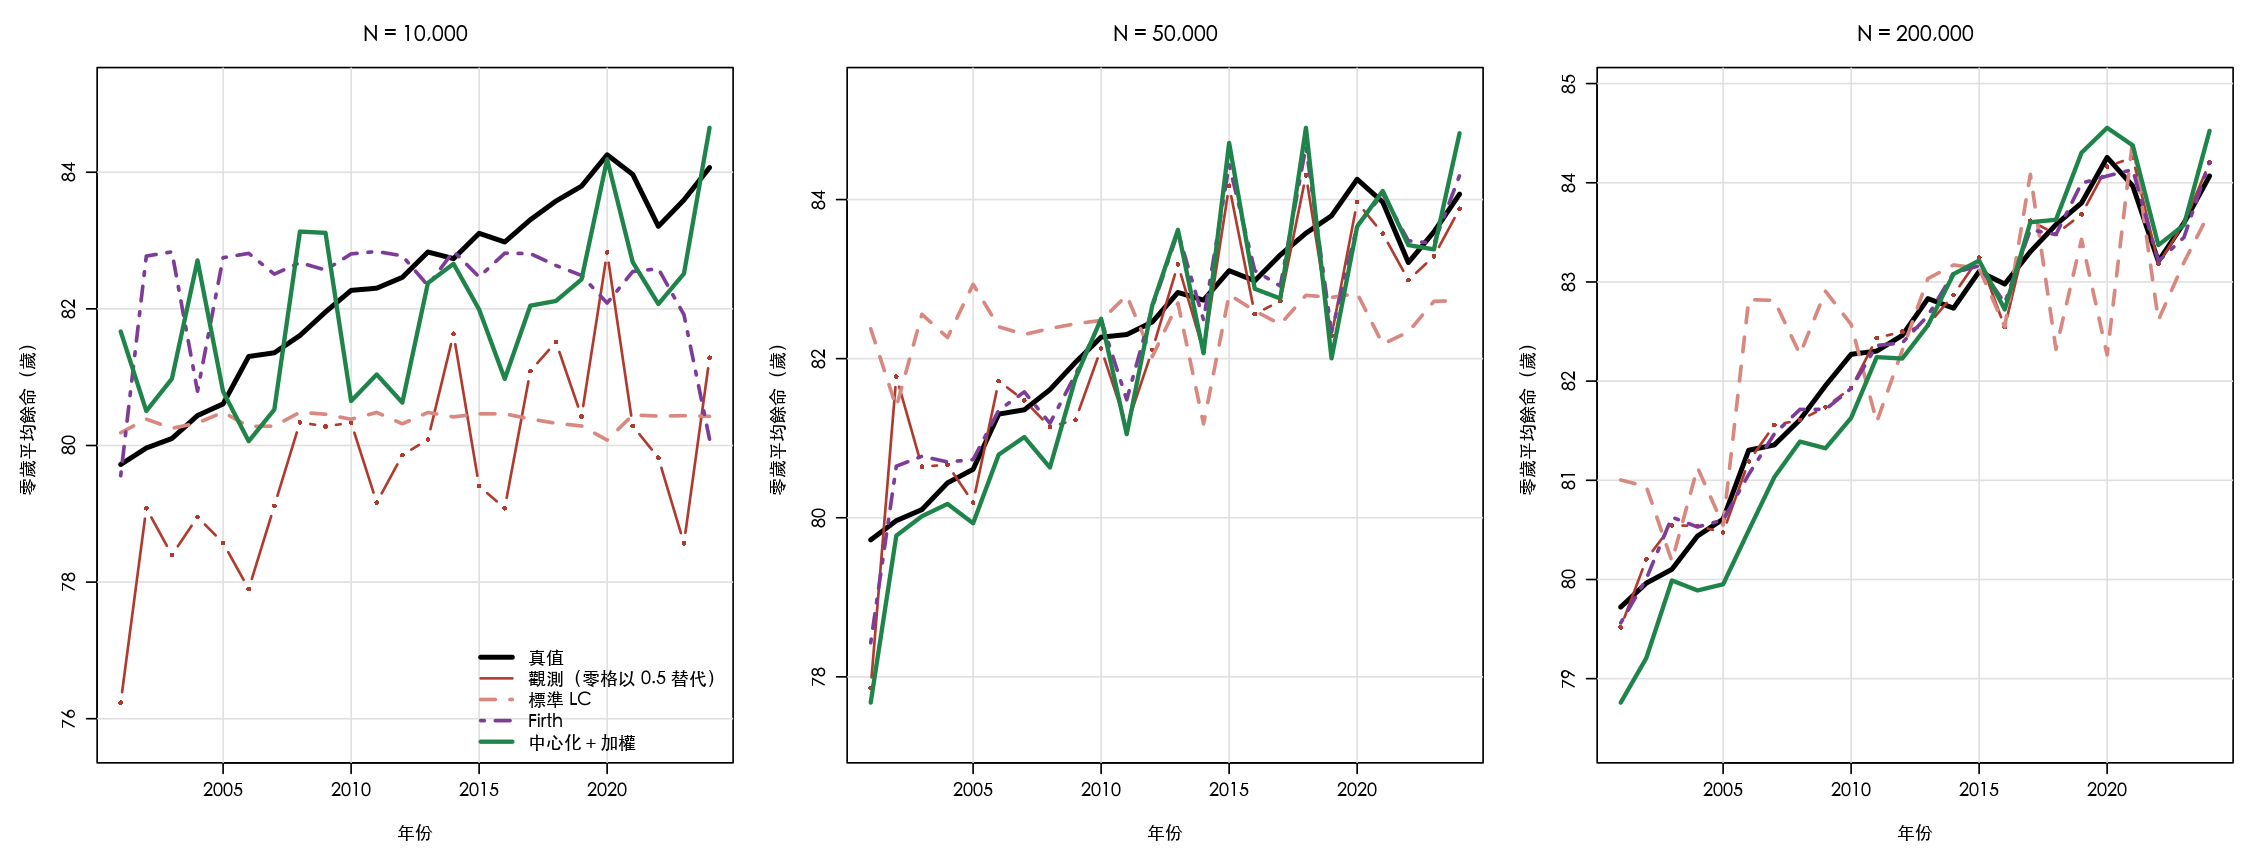
\includegraphics[width=\textwidth]{figT8_e0_oscillation.png}
\caption{零歲平均餘命的逐年序列（單次實現，亂數種子固定）}

{\footnotesize 註：深紅為觀測序列、黑為真值、淺紅虛線為標準 Lee-Carter。}

\label{fig:e0osc}
\end{figure}

觀測序列的震盪相當明顯。
人數一萬時其粗糙度為 $2.266$ 歲，為真值 $0.330$ 歲的 $6.9$ 倍；
逐年變動均值為 $1.304$ 歲，亦為真值 $0.299$ 歲的 $4.4$ 倍。
亦即在一個一萬人的地區，相鄰兩年的平均餘命估計值平均相差一歲以上，
而真實的逐年改善不過 $0.3$ 歲，使用者所看到的年度變化有四分之三是雜訊。
人數二十萬時該比值降為 $2.1$ 倍，震盪顯著緩解。
這與第\ref{sec:intro}節圖~\ref{fig:osc} 所呈現的死亡率震盪一致，
顯示震盪並未因平均餘命是整條曲線的加權平均而被平均掉。

把 Lee-Carter 配適的序列與觀測序列並列，則可看出一個先前未曾注意的現象：
Lee-Carter 並不是把震盪濾掉，而是把震盪換成了趨勢的壓縮。
人數一萬時標準 Lee-Carter 配適序列的粗糙度為 $1.440$，確實低於觀測的 $2.266$；
但其全距只有 $2.898$ 歲，而真值為 $4.534$ 歲，
亦即二十四年間的改善幅度被壓掉了三成六。
其機制可由式~\eqref{eq:astar} 理解：秩一結構以 $\hat\kappa_t$ 承載全部
時間訊號，而人數少時 $\hat\kappa_t$ 的訊號雜訊比下降，
奇異值分解所取的第一組奇異向量因此向零收縮。
換言之，第\ref{sec:valid}節所刻畫的「震盪看得見而偏誤看不見」，
在時間維度上有一個對應的版本，亦即震盪被壓下去的同時趨勢也被壓平，
而後者在單一地區的圖上同樣看不出來。

所提的修正在這一層上沒有改善，甚至更差，這是必須寫下的負面結果。
中心化加權配適的粗糙度在三個規模下分別為 $2.803$、$1.402$、$0.793$，
皆高於標準 Lee-Carter 的 $1.440$、$1.193$、$1.419$；
其全距則為 $8.026$、$6.601$、$6.110$ 歲，皆超過真值的 $4.534$，
亦即由壓縮轉為放大。
原因在於加權版的 $\hat\kappa_t$ 是由加權奇異值分解的右奇異向量回推而得，
其逐年的回推係數隨各年的權重而變，使 $\hat\kappa_t$ 的逐年波動被放大。
這一項缺陷源自本文推導的範圍：第\ref{sec:method}節只處理了 $\hat\alpha_x$ 的
Fisher 不一致與 $\hat\beta_x$ 的擾動分解，而 $\hat\kappa_t$ 並未納入同一個
框架，其加權後的回推只是一個計算上的權宜作法，沒有對應的理論保證。
在死亡率預測的應用中時間參數是外推的依據，因此此一缺陷不能忽略，
第\ref{sec:disc}節將其列為最優先的後續工作。
整體來看，這組表與圖確立了兩件事：平均餘命確實與死亡率一樣在小人口下
劇烈震盪；而 Lee-Carter 模型對此的處理方式是把震盪轉為趨勢的衰減，
所提的修正改善了水準卻尚未改善時間路徑。

\subsection{與參考母體修勻法的比較}\label{sec:smr}

第\ref{sec:ref}指出，死亡率文獻另有一條以參考母體壓抑震盪的路，
其代表為 \citet{lee2003}的 partial SMR。本小節以 \citet[Figure 2]{yue2019}
的七種死亡率比值情境把兩條路並列。
比較的設計如下。小區域的死亡數依第\ref{sec:setup}產生，
其亂數種子只隨人口規模與重複序號變動，於是\textbf{七種情境下的小區域資料
完全相同}；三個不使用參考母體的估計量在各情境下的結果因此一致，
可作為橫向比較的基準線。參考母體的人數取兩百萬，
其真實死亡率設為 $m^{R}_{x,t}=m^{0}_{x,t}/s_x$，
其中 $s_x$ 依序取 $0.8$、$1.0$、$1.2$（型態相同）與隨年齡遞增
（$0.5$ 至 $1.5$）、遞減、V 型、倒 V 型（型態不同）；
參考母體的死亡數同樣由 Poisson 產生，因此其觀測死亡率亦含抽樣誤差。
除 partial SMR 與 Whittaker 比值修勻外，另加入一個只改動零格處理的估計量
（各格保留觀測死亡率，僅把零格填入 $\mathrm{SMR}_t\cdot m^{R}_{x,t}$），
用以分離「參考母體的貢獻有多少來自零格、有多少來自整條曲線的收縮」。

\begin{table}[H]
\centering
\caption{與參考母體修勻法的比較（人數五萬，參考母體兩百萬，重複 100 次）}
\small
\renewcommand{\arraystretch}{1.1}
\begin{tabular}{llrrrrr}
\toprule
情境 & 估計量 & $\alpha$ 中位 & $\alpha$ 最大 & SSE($\beta$) & $e_0$ 偏誤 & $e_0$ 標準差\\
\midrule
\multirow{3}{*}{不用參考母體}
 & 標準 Lee-Carter        & 0.0568 & 0.8658 & 6.7066 & $-1.601$ & 0.610\\
 & Firth          & 0.0077 & 0.1172 & 1.4799 & $-0.171$ & 0.422\\
 & 中心化＋加權   & 0.0223 & 0.0721 & 1.1199 & $+0.003$ & 0.564\\
\midrule
\multirow{3}{*}{$s_x=1.0$（型態相同）}
 & Partial SMR    & \textbf{0.0025} & \textbf{0.0650} & \textbf{0.0486} & $-0.105$ & 0.638\\
 & Whittaker 比值 & 0.0095 & 0.7622 & 6.4063 & $-1.672$ & 0.619\\
 & 零格以 SMR 填補 & 0.0491 & 0.3315 & 1.1273 & $-0.850$ & 0.911\\
\midrule
\multirow{3}{*}{遞增（型態不同）}
 & Partial SMR    & 0.2064 & 0.9033 & 0.0297 & $-1.013$ & 0.569\\
 & Whittaker 比值 & 0.0100 & 0.7531 & 6.9874 & $-1.682$ & 0.672\\
 & 零格以 SMR 填補 & 0.0593 & 0.9098 & 0.7391 & $-1.140$ & 0.869\\
\midrule
\multirow{3}{*}{遞減（型態不同）}
 & Partial SMR    & 0.3313 & 0.7722 & 0.0863 & $+0.613$ & 0.586\\
 & Whittaker 比值 & 0.0123 & 0.7639 & 7.2038 & $-1.649$ & 0.671\\
 & 零格以 SMR 填補 & 0.0318 & 0.2751 & 3.5989 & $-1.033$ & 0.700\\
\bottomrule
\end{tabular}

{\footnotesize 註：三個不使用參考母體的估計量與三個使用者並列，後者分別在型態相同與型態不同的情境下運作。}


\vspace{2pt}
\parbox{0.92\textwidth}{\footnotesize 註：$s_x=0.8$ 與 $1.2$ 的結果與
$s_x=1.0$ 幾乎相同（$\alpha$ 最大偏誤 $0.045$ 與 $0.062$），
V 型與倒 V 型則介於遞增與遞減之間，為節省篇幅不另列，
完整結果見 \texttt{tableM1\_smr\_compare.csv}。}
\label{tab:smr}
\end{table}

在參考母體的年齡型態與目標區域成固定比例時，
partial SMR 優於本文的修正，且優勢相當大。
$s_x=1.0$ 時其 $\alpha$ 最大偏誤為 $0.065$、$\mathrm{SSE}(\beta)$ 為 $0.049$，
而本文為 $0.072$ 與 $1.120$；人數一萬時差距更明顯
（$0.064$ 與 $0.046$ 對 $0.611$ 與 $2.968$），
其零歲平均餘命的偏誤甚至只有 $+0.103$ 歲；本文為 $-1.485$ 歲。
此一結果並不令人意外，但須明白寫出其成因：
在本節的設計中，參考母體的真實死亡率與目標區域只差一個固定的比例常數，
於是 $\mathrm{SMR}\cdot m^{R}_x$ 幾乎就是真值，
而參考母體有兩百萬人、其觀測死亡率的抽樣誤差可忽略。
蓋因如此，該情境是參考母體法最有利的情形，
其結果應視為該法的上界，而非在真實鄉鎮市區應用時可期待的表現。

當年齡型態不同時，partial SMR 的 $\alpha$ 偏誤則急遽惡化，
而本文的修正不受影響。遞增與遞減情境下其 $\alpha$ 偏誤中位數為
$0.206$ 與 $0.331$，為本文 $0.022$ 的九倍與十五倍；
零歲平均餘命的偏誤為 $-1.013$ 與 $+0.613$ 歲，
前者甚至劣於未使用參考母體的 Firth（$-0.171$ 歲）。
其機制可由式~\eqref{eq:psmr} 直接讀出：
$\hat h^2$ 衡量的是兩個母體的整體異質性，而非逐年齡的差異，
因此當小區域某些年齡高於、另一些年齡低於參考母體時，
修勻會把兩者一併朝 $\mathrm{SMR}\cdot m^{R}_x$ 拉，使形狀失真。
此一現象與 \citet[Table 1]{yue2019}所報告的一致，
其「遞增」情境的平均絕對百分比誤差由不修勻的 $28.96\%$ 惡化至 $47.65\%$。

零格的處理方式本身即可解釋偏誤的相當一部分。
只把零格由 $c_0/E$ 改填 $\mathrm{SMR}_t\cdot m^{R}_{x,t}$、其餘各格完全不動，
即使 $\alpha$ 最大偏誤由 $0.866$ 降至 $0.332$、
$\mathrm{SSE}(\beta)$ 由 $6.707$ 降至 $1.127$、
零歲平均餘命的偏誤由 $-1.601$ 歲降至 $-0.850$ 歲；
人數一萬時更由 $2.331$、$9.464$、$-3.753$ 降至 $0.314$、$1.296$、$-0.856$。
據此可知，以標準化死亡比填補零格並不會得到與 $c_0=0.5$ 相同的結果，
兩者相差約一半的偏誤。
此一結果同時是對第\ref{subsec:consistency}推導的另一項支持：
若偏誤的主要來源確實是零格替代，則只改動零格就應可移除其中相當的部分，
而實測正是如此；剩下的另一半則來自非零格的 Jensen 偏誤
（式~\eqref{eq:jensen}），那一部分只有中心化能處理。

表中表現最差的是 Whittaker 比值修勻，其 $\alpha$ 最大偏誤在人數一萬時
為 $2.302$、與標準 Lee-Carter 的 $2.331$ 相去無幾。
這一項的成因須說明，因為它牽涉到本文的實作選擇：
該法在修勻後仍可能給出非正的死亡率，本文依與標準 Lee-Carter 一致的慣例把它截在
$c_0/E_{x,t}$，而在零死亡的年齡該下限恰好生效，使修勻的結果回到零格替代值。
亦即 Whittaker 比值修勻並未處理零格問題，它處理的是非零格的震盪；
此一截斷是分析者的選擇而非該法本身的缺陷，但也凸顯了 partial SMR 的
真正優勢所在，亦即它是三者中唯一在零格上提供正值而不需任何慣例的方法。

尚須指出本節設計的一項限制。七種情境只改動年齡水準 $\alpha_x$ 而未改動
年齡敏感度 $\beta_x$，由 $m^{R}_{x,t}=m^{0}_{x,t}/s_x$ 可知參考母體的
$\beta$ 與 $\kappa$ 與目標區域完全相同，
因此 partial SMR 在 $\mathrm{SSE}(\beta)$ 上的優勢是設計使然，
不應解讀為該法對 $\beta$ 特別有效。完整的比較須另設 $\beta_x$ 不同的情境，
列為後續工作。

這張表所呈現的是兩條路徑的取捨：
參考母體法以「找得到型態相近的參考母體」為代價換取穩定，
本文的修正以「Poisson 假設成立」為代價換取穩定。
前者在參考母體適當時表現更好，但其適當與否無法由目標區域自己的資料判斷；
後者的假設則可由資料檢驗，見第\ref{sec:real}。
兩者並非互斥，第\ref{sec:disc}節將指出以參考母體填補零格再施以中心化
是一個自然的結合方向。

\subsection{模型誤設下的穩健性檢驗}\label{sec:real}

前述各小節的模擬取 $D\sim\text{Poisson}(E\,m^{\text{fitted}})$，
亦即假設 Lee-Carter 模型完全正確，小人口的資料於是不含任何不合模型的結構。
這對檢驗式~\eqref{eq:bform} 本身是恰當的，但未涵蓋一項實務上更重要的
情形，亦即真實資料本來就不完全服從秩一雙線性結構時校正的有效性。
為此本文另設計一項以真實資料為基礎的檢驗。取實際觀測到的全國死亡數
$D^{\text{obs}}_{x,t}$，以 Poisson 抽薄產生小人口：
\begin{equation}\label{eq:thin}
D_{x,t}\sim\text{Poisson}\big(p\,D^{\text{obs}}_{x,t}\big),\qquad
E_{x,t}=p\,E^{\text{obs}}_{x,t},\qquad p=N/N^{\text{obs}} .
\end{equation}
如此小人口繼承臺灣死亡率真實的逐年不規則性，所有偏離秩一結構的部分
都被保留下來。實測顯示該偏離並非可忽略：
$\log(D^{\text{obs}}/E^{\text{obs}})$ 對全國 Lee-Carter 配適值的殘差標準差為
$0.0700$。真值仍取全國資料的 Lee-Carter 配適。

抽薄的方式有兩種可能。二項抽薄
$D\sim\text{Binomial}(D^{\text{obs}},p)$ 與式~\eqref{eq:thin} 的期望值相同，
皆為 $p\,D^{\text{obs}}$，但前者有 $D\le D^{\text{obs}}$ 的上界，
其變異數為 $p(1-p)D^{\text{obs}}$ 而非 $p\,D^{\text{obs}}$。
本文採 Poisson 抽薄，理由是它與式~\eqref{eq:pois} 的分配假設完全一致，
不必另行討論上界與變異數縮減的影響；$p$ 很小時兩者的差異本就可忽略
（本文最大的 $p$ 約為 $0.016$）。

須分別說明式~\eqref{eq:thin} 所打破的假設與所保留的假設。 Poisson 抽薄保持 Poisson 族
（若 $D^{\text{obs}}\sim\text{Poisson}(\mu)$ 則
$D\sim\text{Poisson}(p\mu)$），因此式~\eqref{eq:bform} 的形式不變，
只是 $\mu$ 換成 $p\mu$；被打破的不是 Poisson 假設，而是
「$\mu_{x,t}$ 恰好落在秩一雙線性結構上」這個假設。
這正是要檢驗的那一項，因為 $\hat\mu_{x,t}$ 是由 Lee-Carter 配適算出的，
若真值不在該結構上，$\hat\mu$ 即有系統性誤差，校正也就跟著偏。

\begin{table}[H]
\centering
\caption{真實資料 Poisson 抽薄的結果（重複 100 次，取中位數）}
\small
\begin{tabular}{llrrrrrr}
\toprule
$N$ & 估計量 & $\alpha$ 中位 & $\alpha$ 最大 & SSE($\beta$) & 漂移偏誤 & $e_0$ 偏誤 & $e_0$ 四分位距\\
\midrule
\multirow{5}{*}{\shortstack[l]{$10^4$\\ 零格 216/528}}
 & 標準 Lee-Carter          & 0.1920 & 2.1676 & 7.719 & 0.2510 & $-2.366$ & 0.965\\
 & Poisson MLE       & 0.0724 & 11.3729 & 14.421 & 0.2487 & \textbf{$-0.553$} & 1.043\\
 & Firth            & \textbf{0.0238} & \textbf{0.1725} & 20.455 & 0.2748 & $-1.131$ & \textbf{0.856}\\
 & 中心化           & 0.0481 & 0.3317 & 13.471 & 0.3289 & $-1.460$ & 0.911\\
 & 中心化 $+$ 加權   & 0.1328 & 0.5953 & \textbf{3.671} & \textbf{0.2315} & $-1.365$ & 1.431\\
\midrule
\multirow{5}{*}{\shortstack[l]{$5\times10^4$\\ 零格 91/528}}
 & 標準 Lee-Carter          & 0.0896 & 0.7604 & 6.876 & 0.3520 & $-1.366$ & 0.741\\
 & Poisson MLE       & 0.0087 & 0.1175 & 1.655 & \textbf{0.0230} & \textbf{$-0.155$} & 0.545\\
 & Firth            & \textbf{0.0084} & \textbf{0.0895} & 1.437 & 0.0258 & $-0.204$ & 0.547\\
 & 中心化           & 0.0159 & 0.1542 & 6.856 & 0.3407 & $-1.632$ & 0.737\\
 & 中心化 $+$ 加權   & 0.0471 & 0.3306 & \textbf{1.117} & 0.1148 & $+0.393$ & \textbf{0.630}\\
\midrule
\multirow{5}{*}{\shortstack[l]{$2\times10^5$\\ 零格 23/528}}
 & 標準 Lee-Carter          & 0.0321 & 0.1567 & 1.358 & 0.2139 & $-0.977$ & 1.031\\
 & Poisson MLE       & 0.0063 & 0.0461 & 0.234 & 0.0052 & $+0.024$ & 0.315\\
 & Firth            & \textbf{0.0045} & \textbf{0.0418} & \textbf{0.228} & \textbf{0.0055} & \textbf{$+0.006$} & \textbf{0.314}\\
 & 中心化           & 0.0042 & 0.1541 & 2.873 & 0.2446 & $-1.376$ & 1.183\\
 & 中心化 $+$ 加權   & 0.0347 & 0.3473 & 0.698 & 0.0964 & $+0.640$ & 0.389\\
\bottomrule
\end{tabular}
\label{tab:real}
\end{table}

表~\ref{tab:real} 的設計與第\ref{sec:empmain}相同，
差別只在小人口的死亡數改由實際觀測值抽薄而得，
因此兩張表並列即可分離「模型正確時的表現」與「模型誤設所造成的損失」。
由表中可以看到，校正在真實資料上仍然有效。
$\alpha$ 最大偏誤在三個規模下由 $2.1676$、$0.7604$、$0.1567$
降至 $0.3317$、$0.1542$、$0.1541$，人數一萬與五萬時分別改善 $6.5$ 與 $4.9$ 倍，
與純 Poisson 模擬的 $4.7$ 與 $3.6$ 倍同一量級。
這與式~\eqref{eq:bform} 的性質吻合，蓋因抽薄不破壞 Poisson 族，
而 $b$ 在 $\mu$ 上是平滑的， $\hat\mu$ 的中等誤差不會使 $b(\hat\mu)$
大幅偏離，校正所需的只是 $\hat\mu$ 的量級正確。

$\beta_x$ 的結論同樣不變，而且更為明顯。中心化在三個規模下使
SSE($\beta$) 由 $7.72$、$6.88$、$1.36$ 變為 $13.47$、$6.86$、$2.87$，
在兩個規模下明顯變差；而中心化加上加權則降至 $3.67$、$1.12$、$0.70$，
三個規模皆優於標準 Lee-Carter，改善 $2.1$、$6.2$、$1.9$ 倍。
這與第\ref{sec:betadec}表~\ref{tab:betadec} 的分解一致，
$\beta_x$ 的偏誤九成以上是隨機的，須靠加權而非校正。
真實資料另使標準 Lee-Carter 的 $\beta$ 更差，
人數五萬時 SSE($\beta$) 在真實抽薄下為 $6.88$、在純 Poisson 模擬下為 $4.45$，
差額源自不合秩一結構的成分也被 $\hat\beta$ 吸收；
相對地加權版本在兩種設計下分別為 $1.12$ 與 $1.02$，幾乎不變。
亦即加權不只處理異質變異，也吸收了一部分模型誤設，
這是純模擬設計所看不到的。

不利於本文的部分則出現在與 Firth 的對照上，而且差距大於純模擬。
人數五萬時 Firth 的 $\alpha$ 最大偏誤為 $0.0895$、
零歲平均餘命偏誤為 $-0.204$ 歲，而中心化加權為 $0.3306$ 與 $+0.393$ 歲；
人數二十萬時差距更大（$0.0418$ 與 $+0.006$ 對 $0.3473$ 與 $+0.640$）。
蓋因本文的校正須代入 $\hat\mu_{x,t}$，而 $\hat\mu$ 是由秩一配適算出的，
真實資料不在秩一結構上時 $\hat\mu$ 即有系統性誤差，校正跟著偏；
Poisson 最大概似與 Firth 則直接在計數尺度上配適，
不需要先有一個 $\hat\mu$ 的外部估計。
這是本文修正最明確的適用界線，亦即它依賴的不只是 Poisson 假設，
還包括秩一結構本身大致正確；而這一項限制在第\ref{sec:valid}節的設計下
完全看不到，因為該節的資料恰好落在秩一結構上。

最後須指出，人數一萬時所有方法都不足以支持編表。
即使最佳的 Poisson 最大概似其零歲平均餘命偏誤仍有 $-0.553$ 歲，
而其 $\alpha$ 最大偏誤達 $11.37$、且有 $2\%$ 的重複發散；
Firth 雖穩定，偏誤仍有 $-1.131$ 歲。
在 528 格中有 $216$ 格為零的情形下，資訊量本身已不足，
任何估計量都只能在偏誤與變異之間重新分配，而無法同時降低兩者。
這張表所呈現的是本文結論在模型誤設下的存續程度：
就 $\alpha$ 與 $\beta$ 而言結論不變，
就平均餘命而言則本文的優勢消失，原因可追溯至校正所依賴的 $\hat\mu$
本身來自秩一配適。

\subsection{校正與加權的施加位置，及其在平均餘命上的分工}\label{sec:joint}\label{sec:split}

表~\ref{tab:estcmp} 呈現了一個表面上的取捨：逐格校正把 $\alpha$ 修好卻把
$\beta$ 弄差，加上加權後 $\beta$ 修好了但 $\alpha$ 又退了一些。
兩者看似只能擇一，但第\ref{sec:betadec}的分解顯示並非如此，並指出了出路。
由 Proposition~\ref{prop:beta}，逐格扣除 $b$ 同時做了兩件事：一是移除
$\alpha_x$ 的偏誤，其量為列平均 $\bar b_x$；二是移除 $\beta_x$ 的確定性
擾動 $\Delta_{x,t}=b(\mu_{x,t})-\bar b_x$。但表~\ref{tab:betadec} 已顯示
第二件事的收益很小，$\Delta$ 只佔 $\beta$ 總誤差的一成以下；
而逐格扣除所注入的 $\hat\mu$ 噪音卻進入每一格，對依賴跨格相對大小的
$\beta$ 傷害甚大。既然如此，正確的設計是只做第一件事：
把 $\hat\alpha_x$ 扣掉 $\bar b_x$，而完全不動中心化矩陣。
由式~\eqref{eq:svd}，$\hat\alpha_x$ 是列平均、在奇異值分解之前即已定出，
於是事後扣除 $\bar b_x$ 對 $\hat\beta_x$ 與 $\hat\kappa_t$ 的計算毫無影響；
兩項改善因此可以疊加而不互相干擾。表~\ref{tab:joint} 檢驗此一設計。

\begin{table}[H]
\centering
\caption{逐格校正與僅校正 $\alpha$ 的比較（人數五萬，重複 100 次）}
\small
\begin{tabular}{lrrrrr}
\toprule
估計量 & $\alpha$ 中位 & $\alpha$ 最大 & SSE($\beta$) & 漂移偏誤 & $e_0$ 偏誤（歲）\\
\midrule
標準 Lee-Carter              & 0.0611 & 0.8658 & 4.4494 & 0.3339 & $-1.480$\\
Firth                & 0.0088 & 0.0680 & 1.4102 & \textbf{0.0485} & $-0.282$\\
逐格校正             & 0.0093 & 0.2434 & 8.8335 & 0.3335 & $-1.522$\\
逐格校正 $+$ 加權     & 0.0110 & 0.2524 & \textbf{1.0230} & 0.1381 & $+0.023$\\
僅校正 $\alpha$      & \textbf{0.0063} & \textbf{0.0439} & 4.4494 & 0.3339 & $-1.466$\\
僅校正 $\alpha$ $+$ 加權 & 0.0238 & 0.0715 & 1.1497 & 0.1407 & \textbf{$+0.007$}\\
\bottomrule
\end{tabular}
\label{tab:joint}
\end{table}

結果證實了上述推理，而且有兩處須特別寫明。一方面，僅校正 $\alpha$ 的版本
其 SSE($\beta$) 為 $4.4494$，與標準 Lee-Carter \textbf{完全相同到小數第四位}，這不是巧合，而是因為該作法根本沒有碰到中心化矩陣，$\hat\beta$ 的計算
逐位元一致。另一方面，該版本的 $\alpha$ 最大偏誤為 $0.0439$，\textbf{優於
Firth 的 $0.0680$}，是全表最低；相對地逐格校正為 $0.2434$，
可見逐格扣除所注入的噪音同時也傷害了 $\alpha$ 本身。
把它與資訊加權疊加之後，$\alpha$ 最大偏誤 $0.0715$ 與 Firth 相當、
SSE($\beta$) $1.1497$ 亦與 Firth 的 $1.4102$ 相當，
而零歲平均餘命的偏誤為 $+0.007$ 歲，是全表最接近零者。
在 $\alpha_x$ 與 $\beta_x$ 的估計組成成分上，本小節的結果與
第\ref{sec:betadec}的分解完全相符：$\alpha_x$ 的偏誤為確定性、
可由事後扣除移除；$\beta_x$ 的誤差以隨機成分為主、須由資訊加權壓抑。
據此可知兩者的改善在「校正只施加於列平均、加權只施加於中心化矩陣」
這個條件下能夠疊加。然而，本小節同時證實該疊加並未延伸至時間參數：
漂移偏誤由 $0.3339$ 僅降至 $0.1407$，而僅校正 $\alpha$ 的版本其漂移偏誤
與標準 Lee-Carter 完全相同，可見該項改善全部來自加權而非來自校正。
據此亦可確認 $\kappa_t$ 的偏誤與 $\alpha_x$ 的 Fisher 不一致屬不同來源，
須另行處理，第\ref{sec:disc}節將其列為最優先的後續工作。
圖~\ref{fig:pareto} 把這件事畫成一張取捨圖，橫軸為 SSE($\beta$)、
縱軸為 $\alpha$ 最大偏誤，皆取對數，愈靠左下愈好。

\begin{figure}[H]
\centering
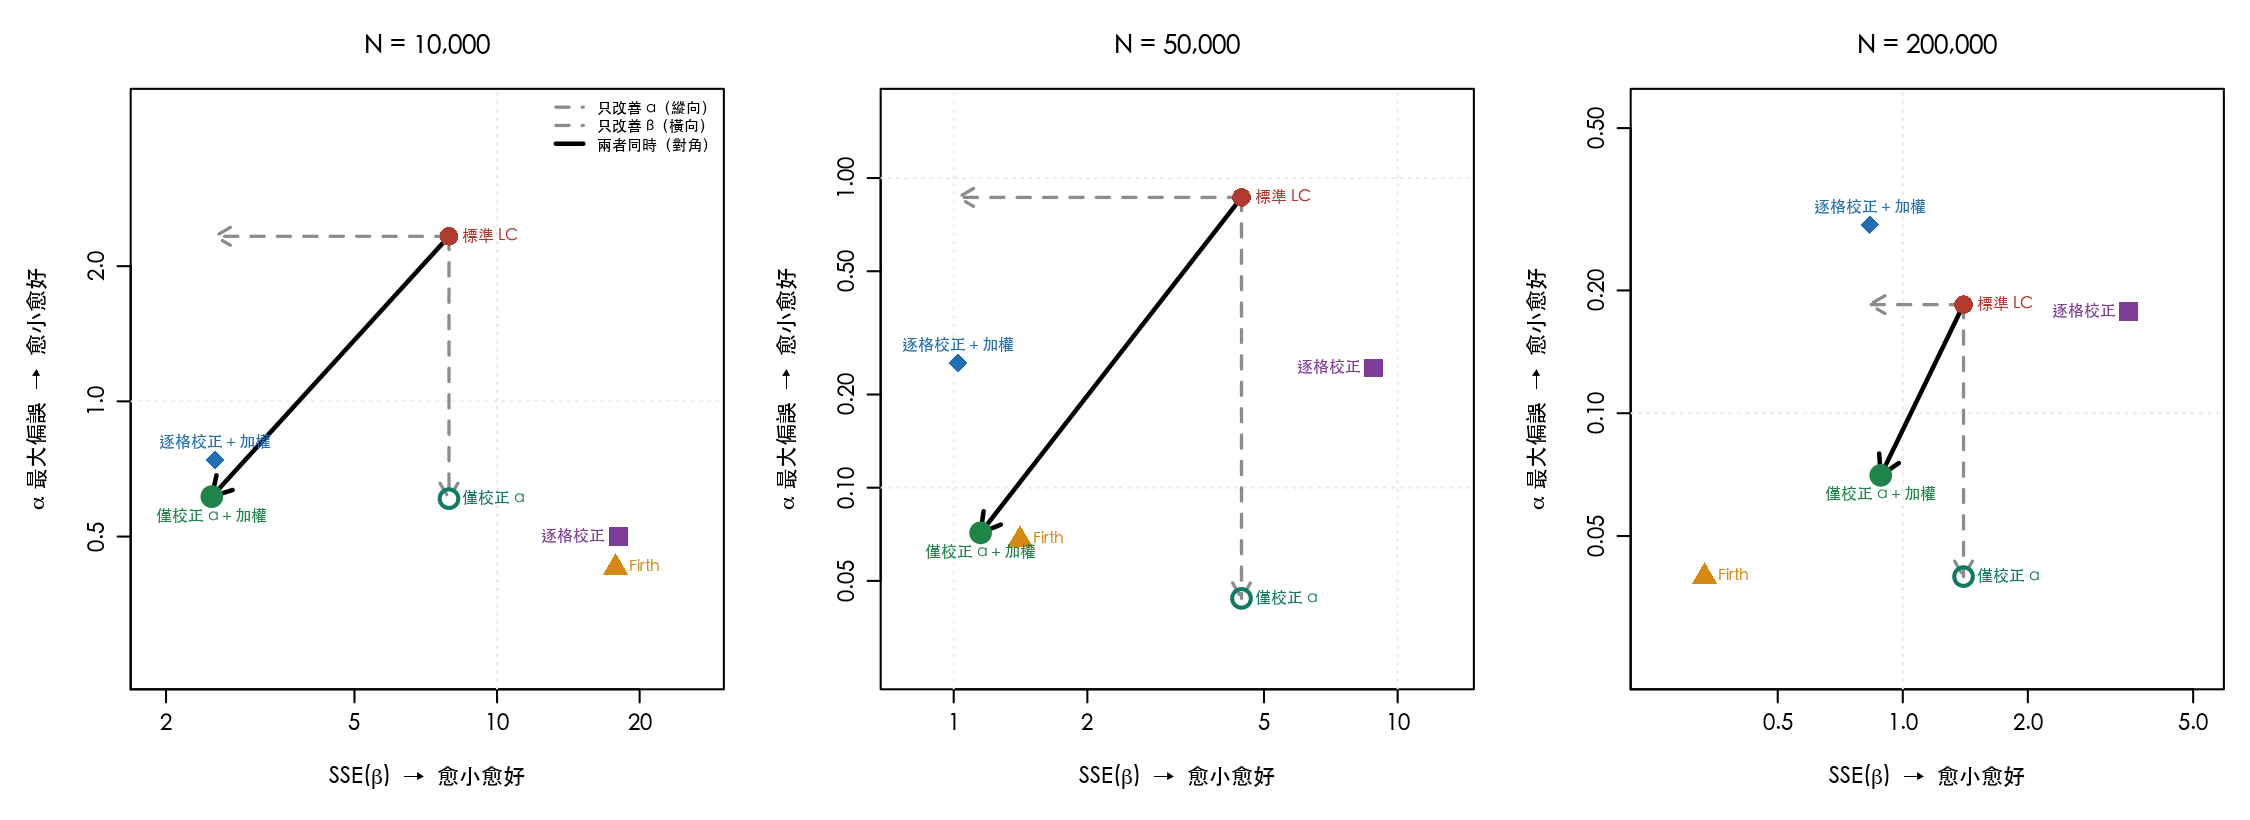
\includegraphics[width=\textwidth]{figT6_pareto.png}
\caption{$\alpha$ 與 $\beta$ 的取捨圖}

{\footnotesize 註：橫軸為 SSE($\beta$)、縱軸為 $\alpha$ 最大偏誤，皆取對數，愈靠左下愈好；箭頭由標準 Lee-Carter 出發。}

\label{fig:pareto}
\end{figure}

圖~\ref{fig:pareto} 的三個箭頭是本小節的摘要。垂直的虛線箭頭表示僅校正
$\alpha$ 只在縱軸上移動，橫軸位置分毫未變；水平的虛線箭頭表示加權主要在
橫軸上移動；而實線的對角箭頭表示兩者疊加後同時往左下走。
人數二十萬時 Firth 仍在更左下的位置，但在五萬與一萬時兩者已相當接近，
而後者正是鄉鎮市區的實際規模。
圖~\ref{fig:jointband} 則把同一件事回到逐年齡的層次。

\begin{figure}[H]
\centering
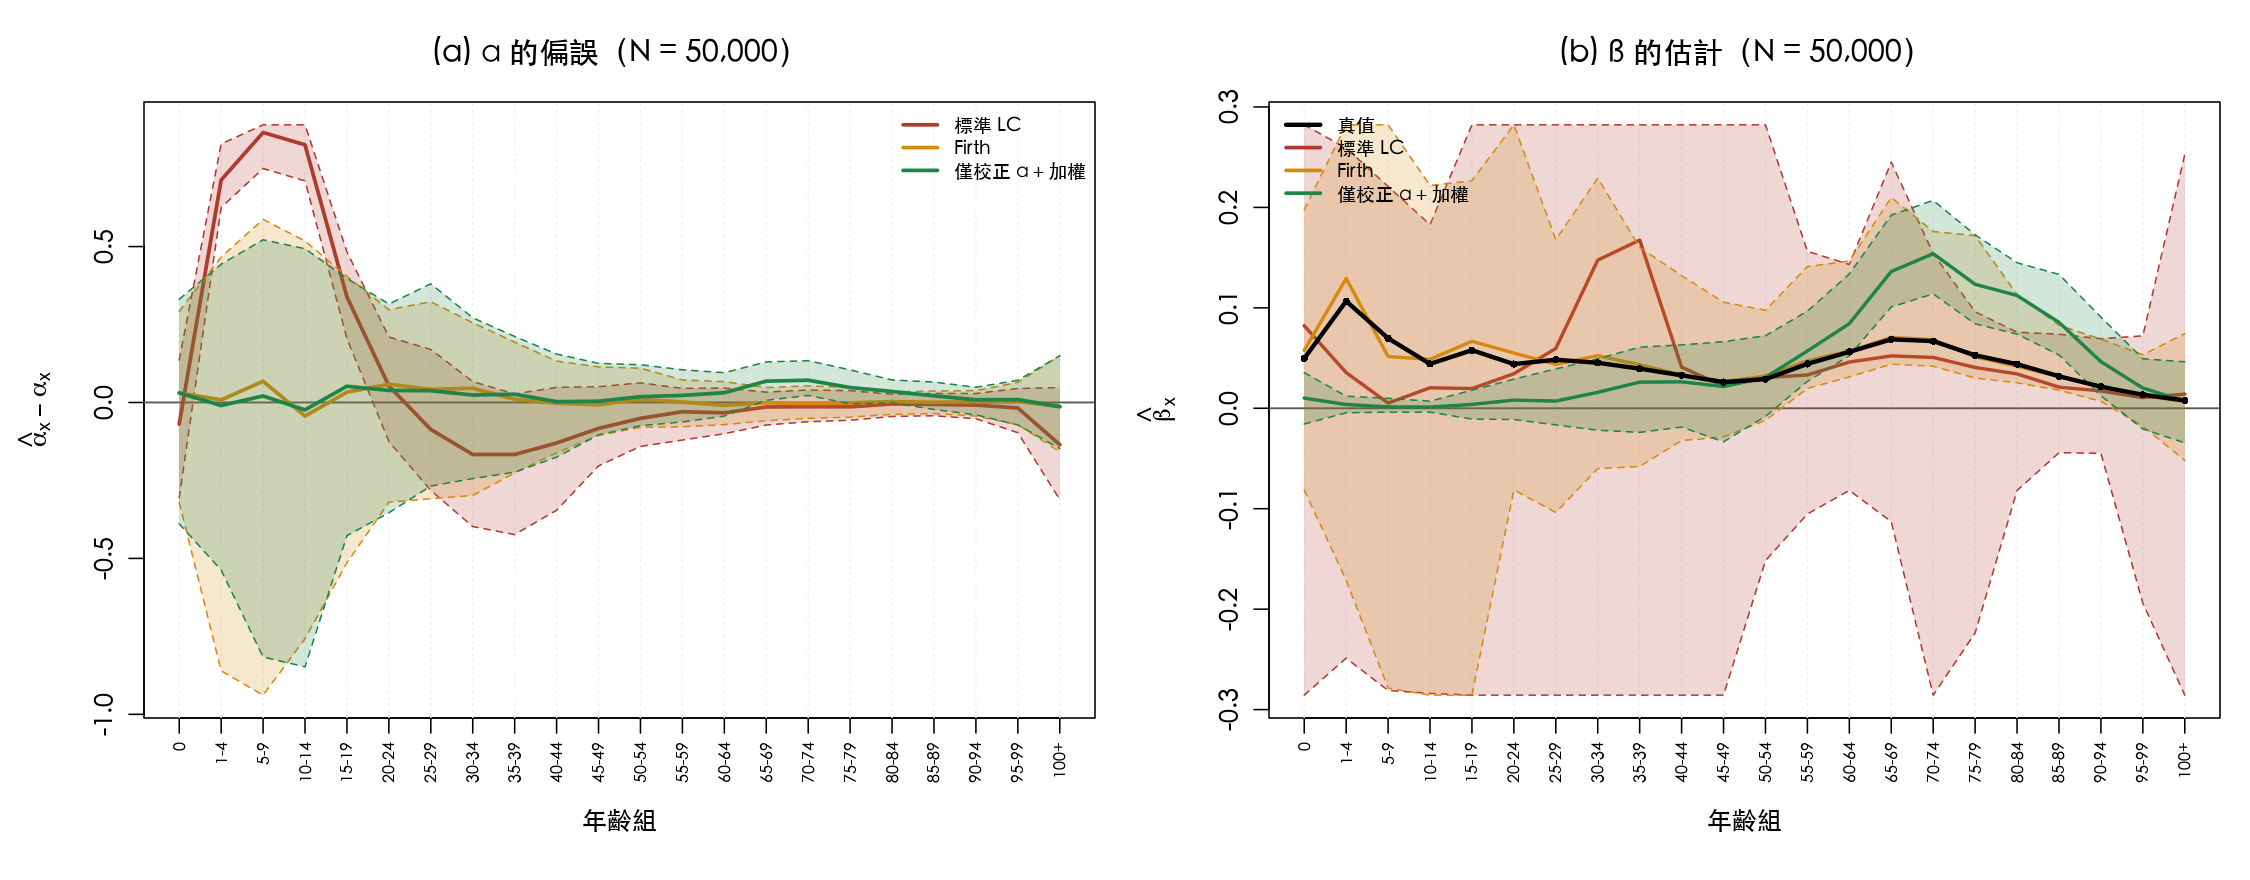
\includegraphics[width=\textwidth]{figT7_joint_band.png}
\caption{標準 Lee-Carter、Firth 與僅校正 $\alpha$ 加權的逐年齡分布（人數五萬，5--95\% 帶）}

{\footnotesize 註：(a) 逐年齡偏誤；(b) $\hat\beta_x$ 的帶。}

\label{fig:jointband}
\end{figure}



使用者最終的標的量通常不是參數本身，而是零歲平均餘命或年金現值這類彙總量，
因此兩項改善各自對該標的量的貢獻須另行說明。
表~\ref{tab:split} 把三個人口規模下的零歲平均餘命偏誤分解為兩段：
由標準 Lee-Carter 到僅校正 $\alpha_x$ 的一段歸於校正，
由僅校正 $\alpha_x$ 到再加資訊加權的一段歸於加權。
閉式預測一欄取第\ref{sec:feas}節的 $\bar b_x$ 代回參考死亡率後重編生命表
所得的差，亦即校正在 $\alpha$ 這一條通道上應有的貢獻。

\begin{table}[H]
\centering
\caption{零歲平均餘命的改善在校正與加權之間的分工（重複 100 次，單位：歲）}
\small
\begin{tabular}{rrrrrrr}
\toprule
$N$ & 標準 Lee-Carter & 僅校正 $\alpha$ & 校正的貢獻 & 閉式預測
 & \ 僅校正 $\alpha$ ＋加權 & 加權的貢獻\\
\midrule
$10^{4}$          & $-3.621$ & $-1.678$ & $\mathbf{+1.943}$ & $+1.640$ & $-1.088$ & $+0.590$\\
$5\times10^{4}$   & $-1.480$ & $-1.466$ & $+0.014$ & $-0.068$ & $+0.007$ & $\mathbf{+1.473}$\\
$2\times10^{5}$   & $-0.899$ & $-1.048$ & $-0.149$ & $-0.136$ & $+0.167$ & $\mathbf{+1.215}$\\
\bottomrule
\end{tabular}

\vspace{3pt}
{\footnotesize 粗體為該列中貢獻較大者。閉式預測為
$e_0\bigl(m^{R}\exp(-\bar b)\bigr)-e_0(m^{R})$，只涵蓋 $\alpha$ 這一條通道。}
\label{tab:split}
\end{table}

表~\ref{tab:split} 的設計是把同一個標的量的改善依施加的位置切開，
以判讀兩項工具各自的槓桿，並與閉式的預測對照。
從表中可以看到，兩項工具的相對重要性\textbf{隨人口規模而換手}。
人數五萬與二十萬時，校正的貢獻為 $+0.014$ 與 $-0.149$ 歲，
而加權的貢獻為 $+1.473$ 與 $+1.215$ 歲，相差兩個數量級；
人數一萬時則相反，校正的貢獻為 $+1.943$ 歲而加權只有 $+0.590$ 歲。
閉式對校正這一段的預測相當準確（$+1.640$ 對 $+1.943$、
$-0.136$ 對 $-0.149$），人數五萬時兩者雖符號相反但量級皆在 $0.07$ 歲以內，
落在一百次重複所能分辨的範圍之外。

此一換手有明確的機制；該機制可由第\ref{sec:feas}節的逐年齡剖面直接讀出。
$\alpha_x$ 的偏誤集中在期望死亡數少的幼年組，而幼年組的死亡率絕對水準極低，
在平均餘命的積分中權重很小；中高齡的 $\bar b_x$ 則因 $\mu$ 大而趨近於零，
人數五萬時 60 至 99 歲各組的 $|\bar b_x|$ 都在 $0.023$ 以內。
兩端都小，平均餘命於是對 $\alpha_x$ 的校正不敏感。
但人數降到一萬時幼年組的 $\bar b_x$ 升至 $+2.3$ 以上，
對應的死亡率被放大十倍，此時幼年組的絕對水準已不再可忽略，
校正的槓桿因此回來。

不明顯之處在於這項分工對實務建議的後果；該後果與直覺相反。
若只看人數五萬的那一列，會得到「實務單位若只能實作一件事，應先做加權」
這個結論；但臺灣 368 個鄉鎮市區中有 217 個的單一性別人數在兩萬以下，
而在該規模下校正才是貢獻較大的一項。
換言之，這項分工的方向\textbf{恰好在實務最需要的規模上翻轉}，
因此不能由單一規模的結果外推。
由以上各項，表~\ref{tab:split} 所表現的是：
校正 $\alpha_x$ 的價值在 $\alpha_x$ 參數本身，亦即跨地區比較年齡型態、
把 $\alpha_x$ 當共變數、或編製逐年齡的費率表；
當標的為單一彙總量時，其槓桿在人數五萬以上很小而在人數兩萬以下很大。
兩項工具都應實作，而若只能擇一，應依目標區域的規模決定。

\partline{三}{限制、意涵與結論}

\section{限制、精算意涵與結論}\label{sec:disc}

\subsection{修正的限制、偏誤的方向與適用的界限}\label{sec:lim}\label{sec:risk}\label{sec:bounds}

本節把前述各小節所顯露的限制集中陳述。
首先是純中心化使 $\beta$ 變差：表~\ref{tab:estcmp} 中其 SSE($\beta$)
為 $18.05$、$8.83$、$3.50$，均大於標準 Lee-Carter 的 $7.92$、$4.45$、$1.40$。
機制是逐格扣除 $b(\hat\mu_{x,t})$ 把 $\hat\mu$ 的估計誤差注入每一格，
而 $\beta$ 的估計依賴跨格的相對大小，於是對這種注入特別敏感，
必須配合加權才能抵銷。這是真實的代價而非實作問題，
也正是正則化「以偏誤換變異數」的另一面：此處交換的方向相反，
是以變異數換偏誤，而在 $\beta$ 上此一交換並不有利。

其次是 Firth 在 $\alpha$ 最大偏誤與平均餘命的均方根誤差上仍有優勢。
就 $\alpha$ 最大偏誤而言，其 $0.4267$、$0.0680$、$0.0398$ 優於逐格中心化的
$0.5008$、$0.2434$、$0.1778$；就平均餘命而言，表~\ref{tab:e0var} 顯示
Firth 的均方根誤差在人數五萬與二十萬時為 $0.532$ 與 $0.277$ 歲，
優於本文的 $0.610$ 與 $0.380$ 歲，其來源是較小的變異數
（$0.478$ 與 $0.275$ 對 $0.613$ 與 $0.326$）。
理由與兩者的方法性質一致：中心化只移除期望值的偏移，每一次實現的偏差仍在，
且不改變變異數；Firth 則在計數尺度上估計，在修正偏誤的同時也收縮了估計量。
這對應預先修正的性質，也說明事後與預先兩路並非等價。本文另掃描了部分扣除（係數 $0.8$ 與 $0.6$），結果一律較完全扣除為差，
因此不存在過度校正，原先「$\hat\mu$ 有誤差因此應保守扣除」的推測不成立。

再者，第\ref{sec:weight}所導出的最適權重另有一項限制：該節所導出的最適權重
式~\eqref{eq:woptmu} 雖然正確，實測上卻與簡單的冪次權重沒有可分辨的差異。
以 $\sqrt{\hat\mu}$、$\hat\mu$ 與式~\eqref{eq:woptmu} 三者相比，
人數二十萬、$c=1.345$ 時 $\beta$ 的平方誤差和分別為 $0.4051$、
$0.4108$、$0.4017$，彼此的差距皆在蒙地卡羅誤差之內；
而同一設定下無加權為 $1.0100$，於是真正有價值的是加權本身的有無，
而非「權重的形式對不對」。解釋是目標函數對權重的冪次相當平坦：
權重的作用是反映 $\sigma_x^2$ 跨三個數量級的差異，三者都足以做到這件事，
其間的差異屬二階。實務上因此取最簡單的 $w=\hat\mu$ 即可，
而式~\eqref{eq:woptmu} 的價值在於它說明了固定冪次原則上不可能最適的原因
這一點在推導上重要，在本資料的量級下則不重要。

此外，本次新增的檢驗另顯露一項限制：\textbf{本文的修正不只依賴 Poisson 假設，
也依賴秩一結構本身大致正確}。第\ref{sec:real}的 Poisson 抽薄顯示，
當資料保留臺灣死亡率真實的不規則性時，中心化加權在人數五萬與二十萬時的
平均餘命偏誤為 $+0.393$ 與 $+0.640$ 歲，而 Firth 為 $-0.204$ 與 $+0.006$ 歲。
原因是 $b(\hat\mu_{x,t})$ 須代入由秩一配適算出的 $\hat\mu$，
而真實資料不在秩一結構上時 $\hat\mu$ 即有系統性誤差。
這項限制在純 Poisson 模擬中完全看不到，因為該設計使資料恰好落在秩一結構上。

另外，資訊加權在死亡數多的年齡反而有害。
表~\ref{tab:ageband} 顯示人數五萬時 $60$ 至 $84$ 歲組的 $\alpha$ 均方根誤差，
單純中心化為 $0.0317$（優於標準 Lee-Carter 的 $0.0357$），加權後則惡化為 $0.0626$。
原因是加權版的 $\hat\alpha_x$ 取加權列平均而非等權列平均，
在各年變異本已很小的年齡只是引入額外的變異。
一個直接的改進是讓權重只作用於 $\beta$ 與 $\kappa$ 的求解，
而 $\alpha$ 維持等權列平均；本文尚未實作此版本。

又，時間參數 $\kappa_t$ 完全未納入本文的框架；其後果已可觀察到。
表~\ref{tab:e0osc} 顯示中心化加權所配適的平均餘命序列，其粗糙度在三個規模
下皆高於標準 Lee-Carter，全距亦由標準 Lee-Carter 的壓縮轉為放大。
此處的推導只處理 $\hat\alpha_x$ 的 Fisher 不一致與 $\hat\beta_x$ 的擾動分解，
$\hat\kappa_t$ 的偏誤與逐年波動尚無對應的刻畫；
在死亡率預測的應用中這一項至關重要，是本文最優先的後續工作。

最後，人數一萬以下時所有方法都不足以支持編表。
表~\ref{tab:e0var} 中該規模下最佳的均方根誤差為 $1.378$ 歲，
而第\ref{sec:popstr}顯示在年輕的人口結構下本文的修正甚至劣於標準 Lee-Carter，
原因是該處的 $\hat\mu$ 本身已無資訊可用，
\textbf{校正在最需要它的時候自動失效}。



前述各節以中性的「偏誤」陳述結果。但在精算的應用中，
審查所關注的不是偏誤的大小，而是它的方向，以及承受該方向的業務線。
以下把前述的解析結果翻成這個角度，所用的數字全部來自
第\ref{sec:feas}節的逐年齡剖面與第\ref{sec:e0var}的震盪分析。

偏誤在不同年齡的方向是相反的；這由 $b(\mu;c_0)$ 的形狀決定，不是巧合。
期望死亡數低於 $\mu^{\ast}=0.9234$ 的年齡，$\alpha_x$ 偏高，死亡率被高估；
人數五萬時 5 至 9 歲組的 $\bar b_x=+0.869$，對應死亡率被放大 $2.38$ 倍，
1 至 4 歲組為 $2.07$ 倍、10 至 14 歲組為 $2.30$ 倍。
期望死亡數高於 $\mu^{\ast}$ 的年齡則 $\alpha_x$ 偏低，死亡率被低估，
但其量級受 $-1/(2\mu)$ 支配而很小：同一規模下 60 至 99 歲各組的死亡率
只被低估 $1\%$ 至 $2\%$。

\begin{table}[H]
\centering
\caption{偏誤方向對各業務線的後果（人數五萬）}
\small
\begin{tabular}{llll}
\toprule
業務線 & 關鍵年齡 & 受 $\alpha_x$ 偏誤的影響 & 主要風險來源與方向\\
\midrule
定期壽險     & 20--60 & 輕微偏高（$\bar b_x$ 由 $+0.04$ 至 $-0.19$） & 無；方向保守\\
年金／退休金 & 60$+$  & 幾乎不受影響（$|\bar b_x|\le0.023$） & $\kappa_t$ 壓縮；\textbf{不審慎}$^{\dagger}$\\
公共衛生指標 & 全年齡 & 透過 $e_0$ 傳遞 & $\kappa_t$ 壓縮為主；低估 $e_0$\\
\bottomrule
\end{tabular}
\vspace{3pt}
{\footnotesize $^{\dagger}$ $\kappa_t$ 壓縮所造成的年金負債低估，
\textbf{不在本文修正的涵蓋範圍內}；本文的校正只處理 $\alpha_x$ 與 $\beta_x$，
而第\ref{sec:e0var}顯示校正後的時間路徑並未改善。}
\label{tab:risk}
\end{table}

表~\ref{tab:risk} 的設計是把逐年齡的偏誤方向對應到各業務線的關鍵年齡，
以判讀承受不審慎方向的業務線。
從表中可以看到，年金與退休金這一列最為要緊；其原因與直覺相反。
$\alpha_x$ 的偏誤在六十歲以上幾乎為零，\textbf{年金負債並不直接受
$\alpha_x$ 偏誤影響}；真正的風險來自時間參數。
第\ref{sec:e0var}的表~\ref{tab:e0osc} 顯示，標準 Lee-Carter 的配適序列
在二十四年間的全距只有真值的六成（人數五萬時 $2.629$ 對 $4.534$ 歲，
人數一萬時 $2.898$ 對 $4.534$ 歲），亦即死亡率的改善幅度被壓掉約四成。
把這個被壓縮的趨勢外推，未來的死亡率會被系統性高估，
年金負債因此被低估，這是不審慎的方向，且其規模可觀。

本文的修正並未解決這一條，甚至在時間路徑上更差。
第\ref{sec:e0var}所記載的負面結果是：中心化加權使配適序列的粗糙度由
$1.193$ 升至 $1.402$、全距由 $2.629$ 放大至 $6.601$（人數五萬），
亦即校正後的時間路徑比標準 Lee-Carter 更不平滑、擺幅更大。
此一結果必須寫進限制，蓋因對年金實務而言這正是最關鍵的一條；
它同時也說明了把 $\kappa_t$ 納入同一框架應排在後續工作第一位的理由。

另有一項與開放年齡組相關的細節。人數五萬時 $100$ 歲以上組的
期望死亡數為 $5.0$，恰落在 $b$ 取極小的鄰域，其 $\bar b_x=-0.119$，
對應死亡率被低估 $11\%$。該組雖人數少，卻決定年金現值的尾端，
而它是六十歲以上唯一偏誤不可忽略的年齡組。
合而觀之，表~\ref{tab:risk} 所表現的是：
就死亡率水準而言本文的偏誤方向對壽險是保守的、對年金幾乎中性；
真正不審慎的方向出在時間趨勢的壓縮；該項不在本文修正的涵蓋範圍內。


除前述三項限制外，另有四項界限須主動寫明，
蓋因它們界定了本文結果的適用範圍。
\textbf{其一，方法依賴秩一雙線性結構，而損失正好落在精算所關心的量上。}
第\ref{sec:real}以真實觀測死亡數的 Poisson 抽薄檢驗模型誤設，
結果顯示 $\alpha_x$ 與 $\beta_x$ 的結論不變（改善 $1.2$ 至 $6.5$ 倍），
但零歲平均餘命的優勢消失：人數五萬時本文的修正為 $+0.393$ 歲而
Firth 為 $-0.204$ 歲，人數二十萬時為 $+0.640$ 歲對 $+0.006$ 歲。
就統計而言這是一項可接受的界限，就精算而言則是要害。
此處不宜淡化，而應寫成一條明確的適用條件：
\textbf{本文的修正適用於標的為參數本身的情形}，例如跨區年齡型態的比較與
費率表的逐年齡結構；\textbf{當標的為平均餘命或年金現值等彙總量、
且資料可能偏離秩一結構時，Firth 的預先修正較為穩健}。

\textbf{其二，本文只有點估計，而監理框架要的是分布。}
償付能力二號的資本要求與國際財務報導準則第 17 號的風險調整，
都不是點估計所能滿足的；本文通篇為點估計。
此一缺口並非無從填補：本研究先前已完成狀態空間 REML 對變異成分低估的處理、
區塊自助法對序列相關的處理，以及 BBP 門檻的模擬校準，
三者都是現成的材料。把它們與本文的點估計修正整合為
「小人口 Lee-Carter 的點估計與區間」，是投稿前優先於再加新方法的工作。

\textbf{其三，適用範圍只涵蓋少數鄉鎮市區。}
第\ref{subsec:grade}的分級顯示，B 級須有單一性別人數九萬六千以上，
而我國 368 個鄉鎮市區中有 299 個少於五萬、217 個少於兩萬。
第\ref{sec:result}節另顯示人數一萬時所有方法都不足以支持單獨編表，
最佳的均方根誤差仍有 $1.378$ 歲，且本文的修正在年輕的人口結構下
甚至劣於標準 Lee-Carter（第\ref{sec:popstr}，$-2.542$ 對 $-1.858$ 歲）。
誠實的推論是本方法把可用範圍往下推了，但沒有移除下限。
此一結論寫成政策建議反而是貢獻，其內容即第\ref{subsec:grade}所列的分級準則。

\textbf{其四，$\kappa_t$ 完全未納入框架，而預測的根本在 $\kappa_t$。}
本文的推導只處理 $\hat\alpha_x$ 的 Fisher 不一致與 $\hat\beta_x$ 的擾動分解。
由精算的角度，這不是「尚未完成的一項」，而是\textbf{這套方法可用於
定價與準備金的前提}：費率與準備金所依據的是外推後的死亡率，
而外推完全由 $\kappa_t$ 的漂移決定。
前文已指出該項的方向對年金不審慎；本文的修正並未改善它。

\subsection{結論與後續工作}\label{subsec:concl}\label{subsec:future}

本文由 $M$-估計、混合模型與 M-分位數 LASSO 三條一般理論的性質，
推導小人口 Lee-Carter 模型的偏誤，得到三項結論。
首先，既有文獻以模擬觀察到的 $\alpha_x$ 偏誤，在 $M$-估計的架構中有一個
明確的名字與一個閉式：它是標準 Lee-Carter 估計方程的\textbf{Fisher 不一致}，
其量為 $b(\mu;c_0)$（Proposition~\ref{prop:fisher}），而 $\hat\alpha_x$ 的偏誤
恰為各格 $b$ 的算術平均（Corollary~\ref{cor:alpha}），且後者是恆等式。
臺灣資料的驗證給出 $1.000$、$1.000$、$0.988$ 的相關係數。
偏誤的大小於是由一個須以模擬估計的現象，轉為一個可以直接計算的量。

另一項是，混合模型的表示式確立了零格替代的統計意義，並給出兩個門檻。
式~\eqref{eq:mix} 顯示每一格是一個混合權重\textbf{已知}的兩成分混合，
因此古典穩健統計為未知污染比例所付的效率代價在此不必付，這是本文選擇中心化而非穩健損失的理由。而把崩潰點理論代入該表示式，
即得中位數失效的解析門檻 $\mu<\ln2$（式~\eqref{eq:ln2}），
與偏誤變號的門檻 $\mu^\ast=0.9234$ 恰成對比：前者是資料的性質，
後者則隨分析者選定的 $c_0$ 移動。

此外，M-分位數 LASSO 的分類說明中心化與既有補救的關係是正交的，
並給出兩項獲得證實的預測：中心化大幅改善 $\alpha_x$，但不改善
$\beta_x$ 與漂移項。後者本身即是結果，它證明小人口 Lee-Carter 的偏誤
至少來自兩個獨立機制，$\alpha_x$ 源於估計方程的中心不正，
$\beta_x$ 源於權重不當。

此外，$\alpha_x$ 與 $\beta_x$ 的小樣本偏誤在特定假設下可否降低，
本文的結論對兩個參數不同，且差別可以量化。
第\ref{sec:betadec}把兩者的偏誤精確分解為確定性與隨機成分：
$\alpha_x$ 的偏誤在人數一萬與五萬時有 $100\%$ 與 $97\%$ 是確定性的，
因此在 Poisson 假設下可由閉式近乎完全移除；$\beta_x$ 的偏誤則只有
$9.2\%$ 與 $5.8\%$ 是確定性的，其餘來自異質變異噪音旋轉主奇異向量，
無論把 $b$ 算得多準都無法處理，須改以加權為之。
於是可降低偏誤的條件是兩個而非一個： Poisson 假設足以處理 $\alpha_x$，
「加權後噪音變異數大致相等」則足以處理 $\beta_x$；後者不由本文的閉式提供。

另外，以真實資料 Poisson 抽薄的檢驗顯示上述結論對模型誤設具有一定的穩健性
（第\ref{sec:real}）。$\alpha$ 最大偏誤的改善幅度在真實抽薄與純 Poisson 模擬
下同為 $1.2$ 至 $6.5$ 倍的量級。一項只有真實資料才顯示出來的發現是：
標準 Lee-Carter 的 SSE($\beta$) 在真實抽薄下較純模擬明顯為差（人數五萬時 $6.88$
對 $4.45$），而加權版本在兩種設計下幾乎不變（$1.12$ 對 $1.02$），
亦即加權不只處理異質變異，也吸收了一部分模型誤設。
但同一節也顯示本文修正的一項界線：真實資料不落在秩一結構上時，
$\hat\mu$ 本身即有系統性誤差，使校正在人數五萬以上時的平均餘命偏誤劣於
Firth。

又，偏誤不只隨人口規模而變，也隨人口的年齡結構而變，而閉式對兩者
一併給出解釋（第\ref{sec:popstr}）。在總人數固定於五萬的條件下，
把年齡結構由 2001 年的全國結構（$65$ 歲以上占 $8.5\%$）換成老化的結構
（$31.7\%$），標準 Lee-Carter 的 $\alpha$ 最大偏誤由 $0.428$ 升至 $1.456$、
零歲平均餘命的偏誤由 $-1.055$ 歲擴大至 $-2.109$ 歲，
其惡化幅度與把人數由五萬降到一萬相當。閉式在三種結構下預測逐年齡偏誤的
相關係數皆在 $0.998$ 以上、迴歸斜率皆在 $0.96$ 至 $1.00$ 之間，
而校正後三種結構的平均餘命偏誤落在 $-0.235$ 至 $+0.066$ 歲之內。
\textbf{這對使用者有直接的意義：分析者只要有曝露數與一組初步的死亡率估計，
就可以在不做任何模擬的情形下事先算出該地區的 Lee-Carter 估計會偏多少，
而人口老化嚴重的鄉鎮市區需要更謹慎地處理。}

另外，偏誤的移除沒有以變異數為代價，這一點可由平均餘命的分布直接讀出
（第\ref{sec:e0var}）。人數五萬時「僅校正 $\alpha$＋加權」使中位偏誤由
$-1.480$ 歲降為 $+0.007$ 歲，而一百次重複的標準差維持在 $0.613$ 歲不變，
均方根誤差因此由 $1.425$ 降為 $0.610$ 歲。
這與中心化的性質一致：它在估計方程上加一個確定性的位移，改變解的位置
而不改變解的隨機波動。相對地，逐格施加的版本因代入 $\hat\mu$ 而使標準差
由 $0.613$ 升至 $0.670$，兩版本的中位偏誤卻幾乎相同，
再次確認離散的增加來自逐格代入而非中心化本身。
同一節另發現平均餘命確實與死亡率一樣會震盪，人數一萬時觀測序列的
二階差分平均絕對值為真值的 $6.9$ 倍；
但 Lee-Carter 配適並不是把震盪濾掉，而是把震盪換成趨勢的壓縮：
其配適序列二十四年間的全距只有真值的六成四。

最後，與 \citet{lee2003}的 partial SMR 修勻比較後，兩條路的取捨得以量化
（第\ref{sec:smr}）。當參考母體的年齡型態與目標區域成固定比例時，
partial SMR 全面優於本文的修正（人數五萬時 $\alpha$ 最大偏誤 $0.065$
對 $0.072$、$\mathrm{SSE}(\beta)$ $0.049$ 對 $1.120$）；
但當型態不同時其 $\alpha$ 偏誤中位數惡化至本文的九至十五倍，
零歲平均餘命的偏誤達 $-1.013$ 與 $+0.613$ 歲。
\textbf{參考母體法以「找得到型態相近的參考母體」為代價換取穩定，
本文的修正以「 Poisson 假設與秩一結構成立」為代價換取穩定；
前者的前提無法由目標區域自己的資料判斷，後者則可以。}
該節另發現只把零格改以標準化死亡比填補、其餘各格完全不動，
即可使人數五萬時的平均餘命偏誤由 $-1.601$ 歲降至 $-0.850$ 歲，
人數一萬時由 $-3.753$ 歲降至 $-0.856$ 歲。
據此可以確認，以標準化死亡比填補零格並不會得到與
$c_0=0.5$ 相同的結果，兩者相差約一半的偏誤；
同時也再次支持「偏誤的主要來源是零格替代」這個推導結論。

把前述各項工具的原始文獻所記載的限制逐一回顧，可以看出本文的結果如何落在
其中。事後修正所載「須最大概似估計值存在」這項限制，
在本問題上確實出現且後果嚴重，Poisson 最大概似在人數一萬時給出 $-13.03$，
而本文由邊際分布推導的作法正是為繞過它而設。
預先修正的限制（$O(n^{-1})$ 的漸近性）同樣出現，Firth 的殘餘偏誤
在人數一萬時仍有 $0.427$，只是遠小於未修正的量級。
穩健損失的兩項限制則一項被繞過、一項被證實：效率代價因污染比例已知
而不必承受，但「污染為少數」的前提在幼年組明確不成立，其比例達 $0.74$，
超過崩潰點所允許的 $50\%$。
正則化的調參限制在本問題上格外嚴重，因為 Lee-Carter 的跨格借力使交叉驗證無合法的
切分方式；而「以偏誤換變異數」的取捨則以另一種形式出現在圖~\ref{fig:bband}
上，加權使 $\beta$ 的帶寬收窄七倍，卻使中線偏離真值。
經驗貝氏收縮的「直接估計量不偏」前提亦不完全成立，
因 $\hat\beta_x$ 本身即含 $9.2\%$ 的確定性偏誤。
混合模型的限制（成分須有密度）使 EM 無從施加，但因 $\pi$ 已知而不構成障礙。
參考母體修勻的限制則在第\ref{sec:smr}得到定量的確認。

就全局而言，本文的貢獻有三項。其一，標準 Lee-Carter 的年齡參數 Fisher 不一致，
而該不一致有一般形式，其在 Poisson 之下為閉式；$\hat\alpha_x$ 的偏誤是一個
有限樣本的恆等式而非漸近近似，且不隨觀測年數增加而消失。
其二，本文導出三個二階解析量，亦即對數尺度的變異數、校正所付的變異數代價，
以及相對於 Poisson 最大概似的效率；三者合起來界定了這一類校正所能達到的
上限，其中效率的損失全程不超過 $12.2\%$。
其三，由於偏誤的計算只需要曝露數與一組粗略的死亡率，本文把它包裝成一個
事前的可行性檢定；此一檢定補上了古典信賴度標準所缺的一半，
蓋因後者控制估計的變異而假設估計量無偏；該假設在本問題上不成立。
本文的範圍則限於年齡水準參數 $\alpha_x$ 的偏誤，其技術理由在於該參數在
雙線性部分被估計之前即已由列平均定出，可以完全在單變數的框架內分析；
時間參數的偏誤與雙線性結構的識別問題不在本文的涵蓋範圍內。



後續工作有六項，依優先序排列。
首先是把 $\hat\kappa_t$ 納入同一個框架。本文的推導只處理 $\hat\alpha_x$ 的
Fisher 不一致與 $\hat\beta_x$ 的擾動分解，而第\ref{sec:e0var}顯示修正後的
$\hat\kappa_t$ 路徑反而更不平滑；在死亡率預測的應用中這一項至關重要。
其次是 $\hat\beta_x$ 的偏誤閉式。$\hat\beta_x$ 與 $\hat\kappa_t$ 為奇異向量，
其偏誤須以逐元的矩陣擾動理論處理（\citealp{abbe2020}），
而非以 \citet{caizhang2018} 的子空間角度界限處理；隨機矩陣一側的對應結果見 \citet{benaych2012} 與 \citet{zhang2022}。
再者是把參考母體與本文的修正結合。第\ref{sec:smr}顯示兩者分別處理零格與
非零格的偏誤，以 $\mathrm{SMR}\cdot m^{R}_x$ 填補零格再施以中心化，
是一個自然且可立即檢驗的組合；此即 0929 討論中所提的問題。
此外是分配假設的放寬。式~\eqref{eq:bform} 依賴 Poisson 假設，
而 \citet{djeundje2010}已指出按年齡與年份分類的死亡資料常有過度離散；
在該情形下式~\eqref{eq:jensen} 的一階項應為 $-\sigma_D^2/(2\mu^2)$
而非 $-1/(2\mu)$，負二項或擬似 Poisson 假設下的對應閉式可同法寫出但尚未做。
另外是比較設計的補全。第\ref{sec:smr}的七種情境只改動年齡水準 $\alpha_x$
而未改動年齡敏感度 $\beta_x$，因此 partial SMR 在 $\mathrm{SSE}(\beta)$ 上的
優勢是設計使然；完整的比較須另設 $\beta_x$ 不同的情境。
最後是真實的鄉鎮市區資料。本文以全國配適為真值作模擬，
並以 Poisson 抽薄檢驗模型誤設，但尚未在真實的小區域資料上驗證，
而該驗證是本方法用於編製鄉鎮市區生命表之前的最後一步。


\section*{參考文獻}
\addcontentsline{toc}{section}{參考文獻}

\noindent\textbf{一、中文部分}
\begin{itemize}[leftmargin=2em, label={}, itemsep=3pt]
  \item[] 王信忠、金碩、余清祥（2012）。小區域死亡率推估之研究。人口學刊，
        45：121-154。
  \item[] 王信忠、余清祥、王子瑜（2017）。臺灣原住民死亡率暨生命表編撰研究。
        人口學刊，55：99-131。
  \item[] 余清祥、王信忠、陳譽騰（2021）。年輪變動比用於小區域人口推估的探討。
        人口學刊，63：99-133。
  \item[] 余清祥、王信忠、呂靖翎（2025）。平均餘命與標準化死亡率之相關分析。
        人口學刊，85-116。
  \item[] 陳政勳、余清祥（2010）。小區域人口推估研究：臺北市、雲嘉兩縣、
        澎湖縣的實證分析。人口學刊，41：153-183。
\end{itemize}

% 英文部分由 BibTeX 依 references.bib 自動產生，依作者姓氏排序。
% 編譯順序：xelatex → bibtex → xelatex → xelatex。
% 中文書目的連接符為「、」，英文樣式無法產生，於是上方仍以 itemize 手寫，
% 其資料庫另存於 references_zh.bib。
\renewcommand{\bibsection}{\vspace{8pt}\noindent\textbf{二、英文部分}\par\vspace{4pt}}
\setlength{\bibsep}{2pt}
\bibliographystyle{apalike}
\bibliography{references}

\end{document}